\documentclass{article} % For LaTeX2e
\usepackage{iclr2023_conference,times}

\usepackage{hyperref}       % hyperlinks
\usepackage{url}            % simple URL typesetting
\usepackage{booktabs}       % professional-quality tables
\usepackage{amsfonts}       % blackboard math symbols
\usepackage{nicefrac}       % compact symbols for 1/2, etc.
\usepackage{microtype}      % microtypography

\usepackage{graphicx}
\usepackage{subcaption}
\usepackage{booktabs} % for professional tables
\usepackage{amsmath}
\usepackage{amsthm}
\usepackage{amssymb}
\usepackage{mathtools}
\usepackage{algorithm}
\usepackage{algorithmic}
\usepackage{thmtools}
\usepackage{thm-restate}
\usepackage{multirow}

\usepackage{hyperref}
%\hypersetup{
	%    hidelinks,
	%}
\usepackage{xcolor}

% Optional math commands from https://github.com/goodfeli/dlbook_notation.
\newcommand{\bX}{\text{\boldmath{$X$}}}

\newcommand{\bw}{\text{\boldmath{$w$}}}
\newcommand{\bW}{\text{\boldmath{$W$}}}
\newcommand{\bH}{\text{\boldmath{$H$}}}
\newcommand{\bmu}{\text{\boldmath{$\mu$}}}
\newcommand{\bHtil}{\tilde{\text{\boldmath{$H$}}}}
\newcommand{\bytil}{\tilde{\text{\boldmath{$y$}}}}
\newcommand{\bxtil}{\tilde{\text{\boldmath{$x$}}}}
\newcommand{\bwtil}{\tilde{\text{\boldmath{$w$}}}}
\newcommand{\bB}{\text{\boldmath{$B$}}}
\newcommand{\bD}{\text{\boldmath{$D$}}}
\newcommand{\bR}{\text{\boldmath{$R$}}}
\newcommand{\br}{\text{\boldmath{$r$}}}
\newcommand{\btheta}{\text{\boldmath{$\theta$}}}
\newcommand{\bQ}{\text{\boldmath{$Q$}}}


\newcommand{\bz}{\boldsymbol{z}}
\newcommand{\bx}{\boldsymbol{x}}
\newcommand{\bk}{\boldsymbol{k}}
\newcommand{\bF}{\boldsymbol{F}}
\newcommand{\bbf}{\boldsymbol{f}}
\newcommand{\be}{\boldsymbol{e}}
\newcommand{\bdelta}{\boldsymbol{\delta}}
\newcommand{\bDelta}{\boldsymbol{\Delta}}
\newcommand{\bxi}{\boldsymbol{\xi}}
\newcommand{\bXi}{\boldsymbol{\Xi}}
\newcommand{\bzeta}{\boldsymbol{\zeta}}
\newcommand{\wpre}{\blodsymbol{w}_{\text{pre}}}
\newcommand{\ba}{\boldsymbol{a}}
\newcommand{\bS}{\boldsymbol{S}}
\newcommand{\bu}{\boldsymbol{u}}
\newcommand{\bb}{\boldsymbol{b}}
\newcommand{\bg}{\boldsymbol{g}}
\newcommand{\by}{\boldsymbol{y}}
\newcommand{\bY}{\boldsymbol{Y}}
\newcommand{\bU}{\boldsymbol{U}}
\newcommand{\bzero}{\boldsymbol{0}}
\newcommand{\bone}{\boldsymbol{1}}

\newcommand{\bl}{\boldsymbol{l}}
\newcommand{\bI}{\boldsymbol{I}}
\newcommand{\bh}{\boldsymbol{h}}
\newcommand{\bq}{\boldsymbol{q}}
\newcommand{\bA}{\boldsymbol{A}}
\newcommand{\bM}{\boldsymbol{M}}
\newcommand{\bV}{\boldsymbol{V}}
\newcommand{\bbP}{\mathbb{P}}
\newcommand{\bbI}{\mathbb{I}}
\newcommand{\bbR}{\mathbb{R}}
\newcommand{\bbC}{\mathbb{C}}
\newcommand{\grad}{\mathrm{grad}}
\newcommand{\bt}{\boldsymbol{t}}
\newcommand{\bv}{\boldsymbol{v}}
\newcommand{\col}{\text{col}}
\newcommand{\imcol}{\text{im2col}}
\newcommand{\row}{\text{row}}
\newcommand{\median}{\mathsf{med}}
\newcommand{\dist}{\text{dist}}
\newcommand{\erf}{\text{erf}}
\newcommand{\erfc}{\text{erfc}}
\newcommand{\vect}{\mathsf{vec}}
\newcommand{\diag}{\mathsf{diag}}
\newcommand{\back}{\mathsf{Back}}
\newcommand{\sW}{\mathsf{W}}
\newcommand{\dirac}{\delta_{\text{Dirac}}}

\DeclareMathOperator*{\argmin}{arg\,min}

\newtheorem{result}{\indent \em Result}\newtheorem{conj}{\textbf{Conjecture}}\newtheorem{assumption}{\textbf{Assumption}}\newtheorem{definition}{\textbf{Definition}}\newtheorem{corollary}{\textbf{Corollary}}\newtheorem{lemma}{\textbf{Lemma}}\newtheorem{theorem}{\textbf{Theorem}}\newtheorem{proposition}{\textbf{Proposition}}\newtheorem{remark}{\textbf{Remark}}\newtheorem{apprx}{\textbf{Approximation}}\newtheorem{example}{\textbf{Example}}\newtheorem{claim}{\textbf{Claim}}\newtheorem{fact}{\indent \em Fact}\newtheorem{step}{\em Step}

\newcommand{\nn}{\nonumber}
\newcommand{\scr}{\scriptstyle}
\newcommand{\disp}{\displaystyle}
\newcommand{\mE}{\mathbb{E}}
\newcommand{\Var}{\mathsf{Var}}
\newcommand{\TV}{\mathsf{TV}}
\newcommand{\cE}{\mathcal{E}}
\newcommand{\cD}{\mathcal{D}}
\newcommand{\cM}{\mathcal{M}}
\newcommand{\cV}{\mathcal{V}}
\newcommand{\cU}{\mathcal{U}}
\newcommand{\cR}{\mathcal{R}}
\newcommand{\cX}{\mathcal{X}}
\newcommand{\cY}{\mathcal{Y}}
\newcommand{\cZ}{\mathcal{Z}}
\newcommand{\cL}{\mathcal{L}}
\newcommand{\cW}{\mathcal{W}}
\newcommand{\cS}{\mathcal{S}}
\newcommand{\cC}{\mathcal{C}}
\newcommand{\cN}{\mathcal{N}}
\newcommand{\cB}{\mathcal{B}}
\newcommand{\cP}{\mathcal{P}}
\newcommand{\cI}{\mathcal{I}}
\newcommand{\cF}{\mathcal{F}}
\newcommand{\cA}{\mathcal{A}}
\newcommand{\cT}{\mathcal{T}}
\newcommand{\cJ}{\mathcal{J}}
\newcommand{\cK}{\mathcal{K}}
\newcommand{\cQ}{\mathcal{Q}}
\newcommand{\cH}{\mathcal{H}}
\newcommand{\cG}{\mathcal{G}}
\newcommand{\cO}{\mathcal{O}}

\newcommand{\tx}{\tilde{x}}
\newcommand{\tg}{\tilde{g}}
\newcommand{\ty}{\tilde{y}}
\newcommand{\tz}{z}
\newcommand{\ts}{\tilde{s}}
\newcommand{\tw}{\tilde{w}}
\newcommand{\tu}{\tilde{u}}
\newcommand{\tR}{\tilde{R}}
\newcommand{\tX}{\tilde{X}}
\newcommand{\tY}{\tilde{Y}}
\newcommand{\tU}{\tilde{U}}
\newcommand{\tP}{\tilde{P}}
\newcommand{\tZ}{z}
\newcommand{\tN}{\tilde{N}}

\newcommand{\chZ}{\check{Z}}
\newcommand{\chN}{\check{N}}
\newcommand{\chR}{\check{R}}

\newcommand{\ut}{\underline{t}}
\newcommand{\ux}{\underline{x}}
\newcommand{\uy}{\underline{y}}
\newcommand{\uu}{\underline{u}}
\newcommand{\uh}{\underline{h}}
\newcommand{\uhy}{\underline{\hat{y}}}
\newcommand{\up}{\underline{p}}

\newcommand{\brw}{\breve{w}}
\newcommand{\brR}{\breve{R}}

\newcommand{\hW}{\hat{W}}
\newcommand{\hR}{\hat{R}}
\newcommand{\hs}{\hat{s}}
\newcommand{\hw}{\hat{w}}
\newcommand{\hY}{\hat{Y}}
\newcommand{\hy}{\hat{y}}
\newcommand{\hz}{\hat{z}}
\newcommand{\hZ}{\hat{Z}}
\newcommand{\hv}{\hat{v}}
\newcommand{\hN}{\hat{N}}
\newcommand{\hhz}{\hat{\hat{z}}}
\newcommand{\hhs}{\hat{\hat{s}}}
\newcommand{\hhw}{\hat{\hat{w}}}
\newcommand{\hhv}{\hat{\hat{v}}}

\newcommand{\baralpha}{\bar{\alpha}}
\newcommand{\barbeta}{\bar{\beta}}
\newcommand{\bargamma}{\bar{\gamma}}
\newcommand{\bartheta}{\bar{\theta}}

\newenvironment{oneshot}[1]{\@begintheorem{#1}{\unskip}}{\@endtheorem}

\providecommand{\lemmaname}{Lemma}
\providecommand{\theoremname}{Theorem}





\providecommand{\lemmaname}{Lemma}
\providecommand{\theoremname}{Theorem}

\makeatother

\providecommand{\lemmaname}{Lemma}
\providecommand{\remarkname}{Remark}
\providecommand{\theoremname}{Theorem}


\newcommand{\fix}{\marginpar{FIX}}
\newcommand{\new}{\marginpar{NEW}}

\usepackage{hyperref}
\usepackage{url}
\newcommand{\yi}[1]{\textcolor{blue}{#1}}


% Authors must not appear in the submitted version. They should be hidden
% as long as the \iclrfinalcopy macro remains commented out below.
% Non-anonymous submissions will be rejected without review.

%\author{Antiquus S.~Hippocampus, Natalia Cerebro \& Amelie P. Amygdale \thanks{ Use footnote for providing further information
%about author (webpage, alternative address)---\emph{not} for acknowledging
%funding agencies.  Funding acknowledgements go at the end of the paper.} \\
%Department of Computer Science\\
%Cranberry-Lemon University\\
%Pittsburgh, PA 15213, USA \\
%\texttt{\{hippo,brain,jen\}@cs.cranberry-lemon.edu} \\
%\And
%Ji Q. Ren \& Yevgeny LeNet \\
%Department of Computational Neuroscience \\
%University of the Witwatersrand \\
%Joburg, South Africa \\
%\texttt{\{robot,net\}@wits.ac.za} \\
%\AND
%Coauthor \\
%Affiliation \\
%Address \\
%\texttt{email}
%}

% The \author macro works with any number of authors. There are two commands
% used to separate the names and addresses of multiple authors: \And and \AND.
%
% Using \And between authors leaves it to \LaTeX{} to determine where to break
% the lines. Using \AND forces a linebreak at that point. So, if \LaTeX{}
% puts 3 of 4 authors names on the first line, and the last on the second
% line, try using \AND instead of \And before the third author name.

%\iclrfinalcopy % Uncomment for camera-ready version, but NOT for submission.
\title{Breaking Correlation Shift via Conditional Invariant Regularizer}
\author{Mingyang Yi$^{1,2,3}$, Ruoyu Wang$^{1,2}$, Jiacheng Sun$^{3}$, Zhenguo Li$^{3}$, Zhi-Ming Ma$^{1,2}$\\
	$^{1}$University of Chinese Academy of Sciences\\
	\texttt{\{yimingyang17,wangruoyu17\}@mails.ucas.edu.cn} \\
	$^{2}$Academy of Mathematics and Systems Science, Chinese Academy of Sciences\\
	\texttt{mazm@amt.ac.cn}\\
	$^{3}$Huawei Noah’s Ark Lab\\
	\texttt{\{sunjiacheng1,li.zhenguo\}@huawei.com}
}
\iclrfinalcopy
\begin{document}
	\date{}
	\maketitle	
	
	\begin{abstract}
		Recently, generalization on out-of-distribution (OOD) data with correlation shift has attracted great attentions. The correlation shift is caused by the spurious attributes that correlate to the class label, as the correlation between them may vary in training and test data. For such a problem, we show that given the class label, the models that are conditionally independent of spurious attributes are OOD generalizable. Based on this, a metric Conditional Spurious Variation (CSV) which controls the OOD generalization error, is proposed to measure such conditional independence. To improve the OOD generalization, we regularize the training process with the proposed CSV. Under mild assumptions, our training objective can be formulated as a nonconvex-concave mini-max problem. An algorithm with a provable convergence rate is proposed to solve the problem. Extensive empirical results verify our algorithm's efficacy in improving OOD generalization.  
	\end{abstract}
	\section{Introduction}
	The success of standard learning algorithms rely heavily on the identically distributed assumption of training and test data. However, in real-world, such assumption is often violated due to the varying circumstances, selection bias, and other reasons \citep{meinshausen2015maximin}. Thus, learning a model that generalizes on out-of-distribution (OOD) data has attracted great attentions. The OOD data \citep{ye2021ood} can be categorized into data with \emph{diversity shift} or \emph{correlation shift}. Roughly speaking, there is a mismatch of the spectrum and a spurious correlation between training and test distributions under the two shifts, respectively. Compared with diversity shift, correlation shift is less explored \citep{ye2021ood}, while the misleading spurious correlation works for training data may deteriorate model's performance on test data \citep{beery2018recognition}. %\citep{geirhos2018imagenet,beery2018recognition,xie2020in,wald2021calibration}.%, which poses a significant challenge for OOD generalization. 
	\par
	The correlation shift says, for the spurious attributes in data, there exists variation of (spurious) correlation between class label and such spurious attributes from training to test data (Figure \ref{fig:waterbirds}). Based on a theoretical characterization of it, we show that given the class label, the model which is conditionally independent of spurious attributes has stable performance across training and OOD test data. Then, a metric \emph{Conditional Spurious Variation} (CSV, Definition \ref{def:csv}) is proposed to measure such conditional independence. Notably, in contrast to the existing metrics related to OOD generalization \citep{hu2020domain,mahajan2021domain}, our CSV can control the OOD generalization error. 
	\par
	% Concretely, our characterization is conducted under data with spurious attributes, and an assumption that given the class label and spurious attributes, the conditional distribution of input is invariant across training and test distribution. With this assumption, we show that, given the class label, for the model that is conditional independent of spurious attributes, they have stable performance across training and OOD test data. Based on this, we propose a metric named \emph{conditional spurious variation} (CSV, Definition \ref{def:csv}) to measure the magnitude of conditional independence between a model and spurious attributes. The sum of the proposed CSV and i.i.d. generalization error is shown to be an upper bound to the OOD generalization error. Thus, a smaller CSV induces a better OOD guarantee. Interestingly, we show by an information-theoretic bound \citep{xu2017information,bu2020tightening} that the conditional independence does not only guarantees the OOD generalization but also improves the i.i.d. generalization ability of the model.    
	\begin{figure}[t]\centering
		\vspace{-0.5in}
		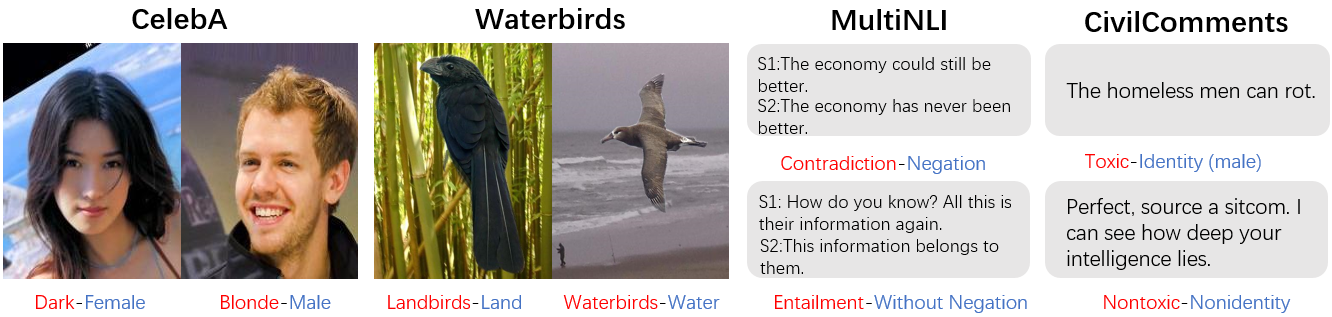
\includegraphics[width=1\textwidth]{./pic/dataset_new.png}
		\vspace{-0.22in}
		\caption{Examples of \texttt{CelebA} \citep{liu2015deep}, \texttt{Waterbirds} \citep{sagawa2019distributionally}, \texttt{MultiNLI} \citep{williams2018broad}, and \texttt{CivilComments} \citep{borkan2019nuanced} involved in this paper. The class labels and spurious attributes are respectively colored with red and blue. Their correlation may vary from training set to test set. More details are shown in Section \ref{sec:experiments}.}
		\label{fig:waterbirds}
		\vspace{-0.3in}
	\end{figure} 
	\par
	To improve OOD generalization, we regularize the training process with estimated CSV. With observable spurious attributes, we propose an estimator to CSV. However, such observable condition may be violated. In this case, we propose another estimator, which approximates a sharp upper bound of CSV. We regularize the training process with one of them, depending on whether the spurious attributes are observable. Our method improves the observable condition in \citep{sagawa2019distributionally}.
	\par
	Under mild smoothness assumptions, the regularized training objective can be formulated as a specific non-convex concave minimax problem. A stochastic gradient descent based algorithm with a provable convergence rate of order $\cO(T^{-2/5})$ is proposed to solve it, where $T$ is the number of iterations. %(can be improved to $\cO(T^{-1/4})$ for small gradient noise as in \citep{lin2020gradient}), where $T$ is the number of update steps.
	\par
	Finally, extensive experiments are conducted to empirically verify the effectiveness of our methods on the OOD data with spurious correlation. Concretely, we conduct experiments on benchmark classification datasets \texttt{CelebA} \citep{liu2015deep}, \texttt{Waterbirds} \citep{sagawa2019distributionally}, \texttt{MultiNLI} \citep{williams2018broad}, and \texttt{CivilComments} \citep{borkan2019nuanced}. Empirical results show that our algorithm consistently improves the model's generalization on OOD data with correlation shifts. 
	%Thus regularize the training process with the proposed CSV can break the spurious correlation. 
	% As the definition of CSV involves spurious attributes, the estimation problem is relatively simple when the spurious attributes are observable. An estimator $\widehat{\rm{CSV}}$ with nice theretical guarantee is proposed for the CSV in this case. Unfortunately, the spurious attributes may be unavailable in practical. In this case, we alternatively estimate a sharp upper bound of it which induces another estimator $\widehat{\rm{CSV}}_{\rm U}$. To improve the OOD generalization capability of the model, we propose to regularize the training process with $\widehat{\rm{CSV}}$ or $\widehat{\rm{CSV}}_{\rm U}$ when the spurious attributes are observable or unobservable respectively. It is worth noting that the regularizer $\widehat{\rm{CSV}}_{\rm U}$ can be computed without any extra information on the spurious attributes or domains, which are widely required in many existing methods \citep{sagawa2019distributionally,arjovsky2019invariant}. Both of the regularized training objectives can be formulated as a non-convex concave minimax problem under mild smoothness assumptions. A stochastic gradient descent based algorithm with proved convergence rate in terms of approximating first-order stationary point is proposed to solve the problem. The convergence rate is of order $\cO(T^{-1/5})$ (can be improved to $\cO(T^{-1/4})$ for small gradient noise as in \citep{lin2020gradient}), where $T$ is the number of update steps. 
	
	\section{Related Works and Preliminaries}
	\subsection{Related Works} 
	\paragraph{OOD Generalization.} The appearance of OOD data \citep{hendrycks2018benchmarking} has been widely observed in machine learning community \citep{recht2019imagenet,schneider2020improving,salman2020unadversarial,tu2020empirical,lohn2020estimating}. To tackle this, researchers have proposed various algorithms from different perspectives, e.g., distributional robust optimization \citep{sinha2018certifying,volpi2018generalizing,sagawa2019distributionally,yi2021improved,levy2020large} or causal inference \citep{arjovsky2019invariant,he2021towards,liu2021heterogeneous,mahajan2021domain,wang2022out,ye2021towards}. \cite{ye2021ood} points out that the OOD data can be categorized into data with \emph{diversity shift} (e.g., \texttt{PACS} \citep{li2018deep}) and \emph{correlation shift} (e.g., \texttt{Waterbirds} \citep{sagawa2019distributionally}), and we focus on the latter in this paper, as we have clarified that it deteriorates the performance of the model on OOD test data \citep{geirhos2018imagenet,beery2018recognition,xie2020in,wald2021calibration}.  
	
	\paragraph{Domain Generalization.} To goal of domain generalization is extrapolating model to test data from unseen domains to capture OOD generalization. The problem we explored can be treated by domain generalization methods as data with different spurious attributes can be regarded as from different domains. The core idea in domain generalization is to learn a domain-invariant model. To this end, \cite{arjovsky2019invariant,hu2020domain,li2018deep,mahajan2021domain,heinze2021conditional,krueger2021out,wald2021calibration,seo2022information} propose plenty of invariant metrics as training regularizer. However, unlike our CSV, none of these metrics controls the OOD generalization error. Moreover, none of these methods capture the invariance corresponds to the correlation shift we discussed (see Section \ref{sec:guaranteed OOD generalization error}). This motivates us to reconsider the effectiveness of these methods. Finally, in contrast to ours, these methods require observable domain labels, and it is usually impractical. The techniques in \citep{liu2021heterogeneous,arpit2019predicting,sohoni2020no,creager2021environment} are also applicable without domain information, but they are built on strong assumptions (mixture Gaussian data \citep{liu2021heterogeneous} and linear model \citep{arpit2019predicting}) or require a high-quality spurious attribute classifier \citep{sohoni2020no,creager2021environment}.
	%so that they can apply unsupervised clustering technique to recover the domain label.  
	
	\paragraph{Distributional Robustness.} The distributional robustness \citep{ben2013robust} based methods minimize the worst-case loss over different groups of data \citep{sagawa2019distributionally,liu2021just,zhou2022model}. The groups are decided via certain rules, e.g., data with same spurious attributes \citep{sagawa2019distributionally} or annotated via validation sets with observable spurious attributes \citep{liu2021just,zhou2022model}. However, \cite{sagawa2019distributionally} finds that directly minimizing the worst-group loss results in unstable training processes. In contrast, our method has stable training process as it balances the objectives of accuracy and robustness over spurious attributes (see Section \ref{sec:regularize training with cv}).
	
	% Intuitively, obtaining OOD generalizable model is learning a model with perfect in-distribution test accuracy and robustness over different spurious attribute. Minimizing the wost-group loss mixes the two goals into one objective, while our regularized objective split the two individual goals.   
	
	% To tackle this, \cite{arpit2019predicting} minimizes the intra-class variance of the model with theoretical framework limited to a linear model. \cite{sagawa2019distributionally} minimizes the worst-case training loss over different groups, while their method is only guaranteed to generalize on the data from a mixture of training distributions. \cite{seo2022information} reduces the mutual information between model and spurious attributes, while the mutual information is hard to compute in practical. In contrast, our methods originate from a general framework, and can be easily applied to distributions  beyond a mixture of training distributions.    
	
	\subsection{Problem Setup}\label{sec:notions}
	We collect the notations in this paper. $\|\cdot\|$ is the $\ell_{2}$-norm of vectors. $\cO(\cdot)$ is the order of a number. The sample $(X, Y)\in\cX\times\cY$, where $X$ and $Y$ are respectively input data and its label. The integer set from $1$ to $K$ is $[K]$. The cardinal of a set $A$ is $|A|$. The loss function is $\cL(\cdot, \cdot):\bbR^{K}\times\cY\rightarrow\bbR^{+}$ with $0 \leq \cL(\cdot, \cdot) \leq M$ for positive $K, M$. For any distribution $P$, let $R_{pop}(P, f) = \mE_{P}[\cL(f(X), Y)]$ and $R_{emp}(P, f) = n^{-1}\sum_{i=1}^{n}\cL(f(\bx_{i}), y_{i})$ respectively be the population risk under $P$ and its empirical counterpart. Here $\{(\bx_{i}, y_{i})\}_{i=1}^{n}$ are $n$ i.i.d. samples from distribution $P$, and $f(\cdot): \cX\rightarrow\bbR^{K}$ is the model potentially with parameter space $\Theta\subset\bbR^{d}$ ($f(\cdot)$ becomes $f_{\btheta}(\cdot)$). For random variables $V_{1}, V_{2}$ with joint distribution $P_{V_{1}, V_{2}}$, $P_{V_{1}}$ and $P_{V_{2}\mid V_{1}}$ are the marginal distribution of $V_{1}$ and the conditional distribution of $V_{2}$ under $V_{1}$. $P_{V_{1}}(v_{1})$ and $P_{V_{2}\mid V_{1}}(v_{1}, v_{2})$ are their probability measures.
	% w.r.t. some dominate measure (w.o.l.g. Lebesgue measure).
	\par
	Suppose the training and OOD test data are respectively from distributions $P_{X, Y, Z}$ and $Q_{X, Y, Z}$. We may neglect the subscript if there is no obfuscation. There usually exists similarities between $P$ and $Q$ that guarantee the possibility of OOD generalization \citep{kpotufe2021marginal}.
	The similarity we explored is that there only exists a correlation shift in the OOD test data formulated as follows. For each input $X$, there exists spurious attributes $Z\in\cZ$ that are not causal to predict class label, but $Z$ is potentially related to class label $Y$. The $Z$ can be some features of $X$ e.g., gender of celebrity in Figure \ref{fig:waterbirds}. The correlation between $Z$ and $Y$ (i.e., spurious correlation) can vary from training to test data, and the one in training distribution may become a misleading signal for the model to make predictions on test data. For example, in the celebrity's face in Figure \ref{fig:waterbirds}, if most males in the training set have dark hair, the model may overfit such spurious correlation and mispredict the male with blond hair. Thus we should learn a model that is robust to correlation shift defined as follows.  
	% the hair color is class label and the gender is spurious attribute, we are desired to learn model that is unrelated to the correlation between them. As the correlation may vary from training to test datasets.  
	\par
	\begin{definition}\label{def:correlation shift}
		Given training distribution $P$, the test distribution $Q\in \cP$ has correlation shift, where 
		\begin{equation}\label{eq:data structual}
			\small
			\begin{aligned}
				\cP = \{Q_{X, Y, Z}: Q_{Y} = P_{Y}, Q_{X\mid Y, Z} = P_{X\mid Y, Z}\}.
			\end{aligned}
		\end{equation}
	\end{definition}
	Our definition characterizes the distributions with correlation shift. The first equality in \eqref{eq:data structual} obviates the mismatching caused by label shift (i.e., $P_{Y}\neq Q_{Y}$) which is unrelated to spurious correlation. More discussions of it are in Appendix \ref{subsec: label shift}. The second equality in \eqref{eq:data structual} states the invariance of conditional distribution of data, given the class label and spurious attributes, which is reasonable as the unstable spurious correlations are decided by the joint distribution of $Y$ and $Z$. Finally, since 
	% all the attributes whose correlations between the label are unstable is contained in $Z$. Finally, since
	\begin{equation}
		\small
		\begin{aligned}
			Q_{X, Y}(\bx, y) & = Q_{X, Y}(\bx\mid y)Q_{Y}(y) = Q_{Y}(y)\int_{\cZ} Q_{X\mid Y, Z}(\bx\mid y,  z)dQ_{Z\mid Y}(z\mid y) \\
			& = P_{Y}(y)\int_{\cZ} P_{X\mid Y, Z}(\bx\mid y,  z)dQ_{Z\mid Y}(z\mid y),
		\end{aligned}
	\end{equation}
	the two constraints in \eqref{eq:data structual} together implies the correlation shift of $Q\in\cP$ is from the variety of conditional distributions $Q_{Z \mid Y}$, which is consistent with intuition. Our definition is different from the ones in \citep{mahajan2021domain,makar2022fairness}, as they rely on a causal directed acyclic graph and the existence of a sufficient statistic such that $Y$ only affects $X$ through it. 
	
	\section{Generalizing on OOD Data}\label{sec:Generalizing on OOD Data Under Spurious Correlation}
	In this section, we show that misleading spurious correlation can hurt the OOD generalization. Then we give a condition under which the model is OOD generalizable. 
	\subsection{Spurious Correlation Misleads Models}
	The common way to train a model is empirical risk minimization \citep[ERM][]{vapnik1999nature}, i.e., approximating the minimizer of $R_{pop}(P,f)$ which generalizes well on in-distribution samples via minimizing its empirical counterpart $R_{emp}(P, f)$. However, the following proposition shows that the minimizer of $R_{pop}(P,f)$ may not generalize well on the OOD data from the other distributions in $\cP$. 
	\begin{restatable}{proposition}{counterexample}
		\label{pro:counter example}
		There exists a population risk $R_{pop}(P, f)$ whose minimizer has nearly perfect performance on the data from $P$, while it fails to generalize to OOD data drawn from another $Q\in\cP$. 
	\end{restatable}
	Similar results also appear in \citep{xie2020in,krueger2021out}, while they are not obtained on the minimizer of population risk. The proof of this proposition is in Appendix \ref{app:proofs in sec generalizing} which indicates that the spurious correlation in training data can become a misleading supervision signal that deteriorates the model's performance on OOD data. Hence, it is crucial to learn a model that is independent of such spurious correlation, even if it sometimes can be helpful in the training set \citep{xie2020in}.  
	\subsection{Conditional Independence Enables OOD Generalization}
	Next, we give a sufficient condition proved in Appendix \ref{app:proofs in sec generalizing} to make the model OOD generalizable. The condition is also necessary under some specific data generating structures \citep{veitch2021counterfactual}.   
	\begin{restatable}{theorem}{thminvariantmodel}\label{thm:conditional independence}
		For model $f(\cdot)$ satisfying $f(X)\perp Z\!\mid \!Y$, the conditional distribution $Y\mid f(X)$ and population risk $\mE_{Q}[\cL(f(X), Y)]$ are invariant with $(X, Y)\sim Q_{X, Y}$ such that $Q\in \cP$.  
	\end{restatable}
	Here $f(X)\!\!\perp \! Z \! \mid \!Y$ means given $Y$, $f(X)$ is conditionally independent of $Z$. Theorem \ref{thm:conditional independence} shows our conditional independence obviates the impact of correlation shift, as the prediction error (gap between $Y$ and $f(X)$, decided by $Y\!\mid \!f(X)$) and population risk of model are invariant over test distributions $Q\in\cP$. Thus we propose to obtain a model that is conditional independent of spurious attributes.
	
%	The prediction error of model is decided by $Y\mid f(X)$, which is invariant over $Q\in \cP$. Thus the prediction error and population risk of model are all invariant over OOD test distributions $Q\in\cP$, which indicates the proposed conditional independence obviates the impact of correlation shift. This theorem motivates us to train a model that is conditional independent of spurious attributes in the sequel. 
	
	%$\mE_{Q}[\cL(f(X), Y)]$ is invariant over $Q\in \cP$, the proposed conditional independence obviates the impact of correlation shift as the variety of $Q\in \cP$ only originates from the conditional distribution $Q_{Z\mid Y}$. The theorem motivates us to train a model that is conditional independent of spurious attributes in the sequel. 
	
	\begin{remark}
		If the spurious attributes are domain labels, the conditional independence in Theorem \ref{thm:conditional independence} becomes the ones in \citep{liu2015deep,hu2020domain,mahajan2021domain}, while they do not explore its correlation with the OOD generalization. Besides, the counterexample in \cite{mahajan2021domain} violates our conditional invariant assumption in \eqref{eq:data structual} and hence is not contrary to our theorem.
	\end{remark}
	\section{Learning OOD Generalizable Model}\label{sec:learning OOD generalizable model}
	In Theorem \ref{thm:conditional independence} we propose a independence condition to break correlation shift. In this section, a metric Conditional Spurious Variation (CSV) is proposed to quantitatively measure the independence. As our CSV can control the OOD generalization error, smaller CSV leads to improved OOD generalization. Finally, two estimators of CSV are proposed, depending on whether spurious attributes are observable. 
	
%	and   and it controls the OOD generalization error. Moreover, a generalization bound on in-distribution data is given to show that conditional independence is not contradicted by in-distribution generalization. Finally, two estimators of our CSV are proposed, depending on whether spurious attributes are observable. 
	\subsection{Guaranteed OOD Generalization Error}\label{sec:guaranteed OOD generalization error}
	Theorem \ref{thm:conditional independence} shows that the conditional independence between the model and spurious attributes guarantees the OOD generalization. We propose the following metric to measure such independence.
	\begin{definition}[Conditional Spurious Variation]\label{def:csv}
		The conditional spurious variation of model $f(\cdot)$ is
		\begin{equation}
			\small
			\begin{aligned}
				\mathrm{CSV}(f) = \mE_{Y}\left[\sup_{z_{1}, z_{2}}\left(\mE_{X}[\cL(f(X),Y)\mid Y, Z = z_{1}] - \mE_{X}[\cL(f(X), Y)\mid Y, Z = z_{2}]\right)\right].
			\end{aligned}
		\end{equation}
	\end{definition}
	% \citep{veitch2021counterfactual,makar2022fairness} also propose criteria to measure the conditional independence. However, in contrast to our criteria, theirs has the following drawbacks. 1): Only can be applied when spurious attributes have two classes. 2): Defined on a Reproducing Hilbert Kernel Space, which depends on the choice of reproducing kernel, thus effect the performance of model. 3): Can not be applied in absence of spurious attributes.
	\par
	As can be seen, CSV is a functional of $f(\cdot)$ which measures the intra-class conditional variation of the model over spurious attributes, given the class label $Y$. It can be computed via training distribution and is invariant across $Q\in\cP$ due to \eqref{eq:data structual}. It is worth noting that the model satisfies the conditional independence in Theorem \ref{thm:conditional independence} has zero CSV but not vice versa. \footnote{Conditional independence is a strong sufficient condition to make model OOD generalizable. However, the proof of Theorem \ref{thm:conditional independence} shows the model that is invariant with spurious correlation $Q(Z\mid Y)$ is sufficient to be OOD generalizable, while the invariance can be characterized by both zero CSV and conditional independence.} However, the following theorem proved in Appendix \ref{app:proofs in sec guaranteed} shows that $\mathrm{CSV}(f)$ is sufficient to control the OOD generalization error. 
	\begin{restatable}{theorem}{boundedgap}\label{thm:bounded gap}
		For any $Q\in \cP$, we have 
		\begin{equation}\label{eq:ood gen bound}
			\small
			\sup_{Q\in\cP}|R_{emp}(f, P) - R_{pop}(f, Q)| \leq \left|R_{emp}(f, P) - R_{pop}(f, P)\right| + \mathrm{CSV}(f)
		\end{equation}
	\end{restatable}
	The $|R_{emp}(f,\! P) \!-\! R_{pop}(f,\! P)|$ is in-distribution generalization error, which is well explored \citep{vershynin2018}. Thus, we upper bound the OOD generalization error via the in-distributional one and CSV. The OOD generalization error is also connected to many other metrics e.g., \citep{hu2020domain,mahajan2021domain,ben2007analysis,ben2010theory,muandet2013domain,ganin2016domain}, but none of them directly control the OOD generalization error. 
	Besides, these metrics are proposed to obtain the invariance over $Z$ as a condition, i.e., invariant $P_{f(X), Y \mid Z}$ or $P_{f(X)\mid Z}$, while the invariances can not handle correlation shift (Definition. \ref{def:correlation shift}). As, 1): invariant $P_{f(X), Y \mid Z}$ implies invariant $P_{Y\mid Z}$ which is incompatible with correlation shift, 2): invariant $P_{f(X)\mid Z}=\int_{\cY} P_{f(X)\mid Z, Y}(f(x)\mid z, y)dP_{Y\mid Z}(y\mid z)$ does not imply invariant $P_{f(X)\mid Y, Z}$ which guarantees OOD generalization.    
	\par
	As our bound \eqref{eq:ood gen bound} involves both CSV and in-distribution generalization error, it motivates us to explore whether the conditional independence is contradicted by the in-distribution generalization. The following information-theoretic bound proved in Appendix \ref{app:proofs in sec guaranteed} presents a positive answer. Let $I(V_{1}, V_{2})$ be the mutual information between variables $V_{1}, V_{2}$, we have the following result. 
	\begin{restatable}{theorem}{gengap}\label{thm:gen gap}
		Let model $f_{\btheta}(\cdot)$ parameterized by $\btheta\in \Theta\subset\bbR^{d}$, and is trained on $\cS=\{(\bx_{i}, y_{i})\}_{i=1}^{n}$ from distribution $P$, with the spurious attributes of $\bx_{i}$ is $z_{i}$. If the learned model $f_{\btheta_{\cS}}(\cdot)\perp \cS_{\bz}\mid \cS_{y}$\footnote{$\btheta_{\cS}$ is the learned parameters depends on training set $\cS$. $f_{\btheta_{\cS}}(\cdot)$ is a random element that takes values in a functional space (i.e., model space), details can be referred to \citep{shiryaev2016probability}.} 
		\begin{equation}\label{eq:gen bound}
			\small
			\cE_{\text{gen}}(f_{\btheta_{\cS}}, P) \leq \inf_{g}\sqrt{\frac{M^{2}}{4n}\left(I(\cS_{\bx - g(z)}, \cS_{y}; f_{\btheta_{\cS}}\mid \cS_{y}, \cS_{g(z)}) + I(\cS_{y}; f_{\btheta_{\cS}})\right)},
		\end{equation}
		where $\cE_{\text{gen}}(f_{\btheta_{\cS}}, P) = |\mE[R_{emp}(f_{\btheta_{\cS}}, P)] - R_{pop}(f_{\btheta_{\cS}}, P)|$, $g(\cdot)$ is any measurable function, $\cS_{\bx - g(z)} = \{\bx_{i} - g(z_{i})\}_{i=1}^{n}$, $\cS_{y} = \{y_{i}\}_{i=1}^{n}$. 
	\end{restatable}
	Our bound improves the classical result $\cE_{gen}(f_{\btheta_{\cS}}, P)\leq \sqrt{M^{2}I(\cS, \btheta_{\cS})/4n}$ without conditional independence \citep{steinke2020reasoning}, because taking $g(\cdot)$ as a constant function, then applying data processing inequality \citep{xu2017information} in r.h.s. of \eqref{eq:gen bound}, it becomes $\sqrt{M^{2}I(\cS, \btheta_{\cS})/4n}$. The bound indicates the model $f_{\btheta_{\cS}}(\cdot)$ that is conditional independent of spurious attribute (we aim to capture) is not in contradiction with in-distribution generalization. Thus, due to Theorem \ref{thm:bounded gap}, less conditional independence with spurious attributes of model improves the OOD generalization bound.
	
	\subsection{Estimating CSV with Observable Spurious Attributes}\label{sec:estimators of CSV}
	As smaller CSV enables improved OOD generalization, we propose to regularize the training process with it. Suppose we have $n$ i.i.d. $\{(\bx_{i}, y_{i})\}_{i=1}^{n}$ training samples with spurious attributes $\{z_{i}\}_{i=1}^{n}$ from $P$. Before our analysis, we need the following two mild assumptions in the sequel. 
	\begin{assumption}\label{ass:feature space}
		The class label and spurious attributes are discrete, i.e., the $\cY = [K_{y}]$ and $\cZ = [K_{z}]$ for some positive integers $K_{y}, K_{z}$. Besides that, the number of observations $A_{kz} = \{i: y_{i}=k, z_{i}=z\}$ from each pair of $(k, j)\in[K_{y}]\times [K_{z}]$ is $|A_{kz}| = n_{kz} >0$.
	\end{assumption}
	\begin{assumption}\label{ass:Lip}
		The model is parameterized by $\btheta\in\Theta\subset\bbR^{d}$. The loss function $\cL(f_{\btheta}(\bx), y)$ is Lipschitz continuous and smooth w.r.t. $\btheta$ with coefficient $L_{0}$ and $L_{1}$, i.e., for any $(\bx, y)\in\cX\times\cY$, and $\btheta_{1}, \btheta_{2}\in\Theta$,
		\begin{equation}
			\small
			\begin{aligned}
				\left|\cL(f_{\btheta_{1}}(\bx), y) - \cL(f_{\btheta_{2}}(\bx), y)\right| \leq L_{0}\|\btheta_{1} - \btheta_{2}\|;\\
				\left\|\nabla_{\btheta}\cL(f_{\btheta_{1}}(\bx), y) - \nabla_{\btheta}\cL(f_{\btheta_{2}}(\bx), y)\right\| \leq L_{1}\|\btheta_{1} - \btheta_{2}\|.
			\end{aligned}
		\end{equation}
	\end{assumption}
	In Assumption \ref{ass:feature space}, we require the spurious attributes space is finite. This is explained as $Z$ is a ``label" of spurious attributes, e.g., the gender label ``male" or ``female" in \texttt{CelebA} dataset (Figure \ref{fig:waterbirds}) when classifying hair color. Assumption \ref{ass:feature space} also requires the data with all the possible combinations of the label and spurious attributes are collected in the training set. This is a mild condition since we do not restrict the magnitude of $n_{kz}$. For example, to satisfy this, we can synthetic some of the missing data by generative models as in \citep{wang2022out,zhu2017unpaired}. 
	\par
	% Thus the empirical risk is $R_{emp}(f_{\btheta}, P)$, we denote it as $R_{emp}(\btheta)$ to simplify the notation. One can verify that the number of samples $n$ is $\sum_{(k, j)\in[K_{y}]\times[K_{z}]}n_{k, j} > [K_{y}]\cdot[K_{z}]$. 
	Let $\cL_{kz}(f_{\btheta}) = \mE[\cL(f_{\btheta}(X), k)\mid Y=k, Z=z]$, $\hat{\cL}_{kz}(f_{\btheta})$ $ = (1 / n_{kz})\sum_{i\in A_{kz}}\cL(f_{\btheta}(\bx_{i}), k)$, and $\hat{p}_{k} = n_{k} / n$ with $n_{k}=\sum_{z\in[K_{z}]}n_{kz}$. Then the following empirical counterpart of CSV 
	\begin{equation}\label{eq:empirical csv}
		\small
		\widehat{\rm{CSV}}(f_{\btheta}) = \sum\limits_{k = 1}^{K_{y}}\sup_{z_{1}, z_{2}\in[K_{z}]}\left(\hat{\cL}_{kz_{1}}(f_{\btheta}) - \hat{\cL}_{kz_{2}}(f_{\btheta})\right)\hat{p}_{k}
	\end{equation}
	is a natural estimator to CSV. The following theorem quantify its approximation error. 
	\begin{restatable}{theorem}{genbound}\label{thm:gen bound}
		Under Assumption \ref{ass:feature space} and \ref{ass:Lip}, if  $\inf_{k\in[K_{y}], z\in[K_{z}]} n_{kz} / n_{k} = \cO(1)$, then
		\begin{equation}\label{eq:gen bound order}
			\small
			\mathrm{CSV}(f_{\btheta}) \leq \widehat{\rm CSV}(f_{\btheta}) + \cO\left(\frac{\log{(1/\delta)}}{\sqrt{n}}\right) 
		\end{equation}
		holds with probability at least $1 - \delta$ for any $\btheta\in\Theta, \delta > 0$.
	\end{restatable}
	This theorem implies that CSV is upper bounded by $\widehat{\rm CSV}(f_{\btheta})$. As shown in the proof in Appendix \ref{app: proofs in sec:estimators of CSV}, we hide a factor related to covering number \citep{vershynin2018} of the hypothesis space in the numerator of $\cO\left(\log{(1/\delta)}/\sqrt{n}\right)$ in \eqref{eq:gen bound order}. The hidden factor is of order $\sqrt{d}$ \citep{wainwright2019}. Thus, more samples are required to estimate CSV in high-dimensional space. Besides that, if the condition $\inf_{k,z}n_{kz} / n_{k} = \cO(1)$ does not hold, the order of error is $\cO(1 / \sqrt{\min_{k, z}n_{kz}})$ (see Appendix \ref{app: proofs in sec:estimators of CSV} for details). 
	
	\subsection{Estimating CSV with Unobservable Spurious Attributes}\label{sec:estimating without spurious attributes}
	Computing the empirical CSV \eqref{eq:empirical csv} requires observable spurious attributes which may not be available in practice \citep{liu2021just}. Thus, we need to estimate CSV in the absence of spurious attributes.
	\par
	Let $P_{kz} = P_{X\mid Y = k, Z = z}$ be the conditional distributions of $X$ with $Y, Z$ given. The core difficulty of estimating CSV with unobservable spurious attributes is to estimate $\sup_{z}{\mE}_{P_{kz}}[\cL(f_{\btheta}(X), k)] - \inf_{z}{\mE}_{P_{kz}}[\cL(f_{\btheta}(X), k)]$
	via $n_{k}$ independent samples $\{(x_{i}, y_{i})\}_{i\in A_{k}}$ drawn from a mixture distribution $P_{k} = \sum_{z\in[K_{z}]}\pi_{kz}P_{kz}$. Here  $A_{k}=\bigcup_{z\in[K_{z}]}A_{kz}$ for $k\in[K_{y}]$, $P_{k} = P_{X\mid Y=k}$, $\pi_{kz} = P_{Z\mid Y}(Z = z \mid Y = k)$, and we can not specify the data in $A_{k}$ is from which of $A_{kz}$. To proceed, suppose $\pi_{kz} \geq c > 0$, which is a necessary condition for Assumption \ref{ass:feature space} to hold. We show in Appendix \ref{app:proof of sec:estimating without spurious attributes} that the quantile conditional expectation 
	\begin{equation}\label{eq:quntile estimator}
		\small
		\begin{aligned}
			\mE_{P_{k}}[\cL(f_{\btheta}(X), k)\mid \cL(f_{\btheta}(X), k)\geq q_{P_{k}}(1 - c)] - \mE_{P_{k}}[\cL(f_{\btheta}(X), k)\mid \cL(f_{\btheta}(X), k)\leq q_{P_{k}}(c)]
		\end{aligned}
	\end{equation}
	is an upper bound (which is sharp for $K \geq 3$) of $\sup_{z}{\mE}_{P_{kz}}[\cL(f_{\btheta}(X), k)] - \inf_{z}{\mE}_{P_{kz}}[\cL(f_{\btheta}(X), k)]$. Here $q_{P_{k}}(\cdot)$ is the quantile function defined as $q_{P_{k}}(s) = \inf\{p: P_{k}(\cL(f_{\btheta}(X), k) \leq p) \geq s\}$. For large $n_{k}$, we must have $\pi_{kz}\geq 1/n_{k} = c$ for each $z\in[K_{z}]$. Thus by substituting the expectation on $P_{k}$ in \eqref{eq:quntile estimator} with its empirical counterpart for $c = 1/n_{k}$, we get the the following estimator
	\begin{equation}\label{eq:estimator without spurious attribute}
		\small
		\widehat{\rm{CSV}}_{\rm U}(f_{\btheta}) \!= \!\sum_{k=1}^{K_{y}}\!\left(\max_{i\in A_{k}}\!\cL(f_{\btheta}(\bx_{i}), k) \! - \!\min_{i\in A_{k}}\!\cL(f_{\btheta}(\bx_{i}), k)\right)\hat{p}_{k}. \!
	\end{equation}
	The subscript ``$\rm U$'' means ``unobservable spurious attributes''. Besides that, the $\widehat{\rm{CSV}}_{\rm U}(f_{\btheta})$ is an upper bound to the estimator 
	% with observable spurious attributes 
	$\widehat{\rm{CSV}}(f_{\btheta})$, which is another straightfoward way to obtain it.
	
	\section{Regularizing Training with CSV (RCSV)}\label{sec:regularize training with cv}
	\begin{algorithm}[t!]

		\caption{Regularize training with CSV.}
		\label{alg:sgd}
		\textbf{Input:} Training set $\{(\bx_{i}, y_{i})\}_{i=1}^{n}$, number of labels $K_{y}$ and spurious attributes $K_{z}$, 
		% batch size $S$, learning rate $\eta_{\btheta}$, 
		training steps $T$, model $f_{\btheta}(\cdot)$ parameterized by $\btheta$. Initialized $\btheta_{0}, \{\bF^{k}_{0}\}$. Positive regularization constant $\lambda$, surrogate constant $\rho$, and correction constant $\gamma$. Estimators $\hat{R}_{emp}(f_{\btheta}, P)$ to $R_{emp}(f_{\btheta}, P)$, $\hat{\bF}^{k}(\btheta)$ to $\bF^{k}(\btheta)$.
		
		\begin{algorithmic}[1]
			\FOR    {$t=0, \cdots ,T$}
			%				\STATE  {Randomly sample a mini-batch $\cS = \{(x_{t_{i}}, y_{t_{i}})\}_{i=1}^{S}$.}		
			\STATE  {\textbf{Solve the maximization problem:}}
			\FOR    {$k=1, \cdots, K_{y}$}
			\STATE  {$\bF^{k}_{t + 1} = (1 - \gamma)\bF^{k}_{t} + \gamma\hat{\bF}^{k}(\btheta(t))$;}
			\STATE  {$\bu_{k}(t + 1) = \mathrm{Softmax}(\bF^{k}_{t + 1} / \rho)$.}
			\ENDFOR 
			\STATE  {\textbf{Minimization step via SGD:}}
			\STATE  {$\btheta(t + 1) = \btheta(t) -  \eta_{\btheta}\sum\limits_{k = 1}^{K_{y}}\hat{p}_{k}\nabla_{\btheta}(\hat{R}_{emp}(f_{\btheta(t)}, P) + \lambda\bu_{k}(t + 1)^{\top}\bF_{t + 1}^{k})$.}
			\ENDFOR
		\end{algorithmic}
	\end{algorithm}
	
	The previous results have claimed that the model with small CSV generalizes well on OOD data. On the other hand, Theorem \ref{thm:gen bound} and discussion in Section \ref{sec:estimating without spurious attributes} have approximated the CSV via $\widehat{\rm{CSV}}(f_{\btheta})$ and $\widehat{\rm{CSV}}_{\rm U}(f_{\btheta})$, respectively. Thus we can regularize the training process with one or the other to improve the OOD generalization, depending on whether the spurious attributes are observable. 
	\par
	It is notable that both of the regularized training objectives can be formulated as the following minimax problem for positive constants $m$ and  $\lambda$
	% 	Both of the regularized optimization are special case the following minimax problem.
	%We consider the minimax problem 
	\begin{equation}\label{eq:minimax problem}
		\small
		% 		\min_{\btheta\in\Theta}\sum_{k=1}^{K_{y}}\hat{p}_{k}\left(\frac{1}{n_{k}}\sum_{i\in A_{k}} \cL(f_{\btheta}(\bx_{i}), y_{i}) \!+\! \lambda \max_{\bu\in\Delta_{K_{z}^{2}}}\bu^{\top}\bF^{k}(\btheta)\right),    
		\min_{\btheta\in\Theta}\sum_{k=1}^{K_{y}}\hat{p}_{k}\left(R_{emp}(f_{\btheta}, P) \!+\! \lambda \max_{\bu\in\Delta_{m}}\bu^{\top}\bF^{k}(\btheta)\right).
	\end{equation}
	Here $\Delta_{m} = \{\bu = (u_{1},\dots, u_{m})\in\bbR^{m}_{+}: \sum_{i}u_{i} = 1\}$, $\bF^{k}(\btheta)\in\bbR^{m}$, and each dimension of $\bF^{k}(\btheta)$ is Lipschitz continuous function with Lipschitz gradient. Under Assumption \ref{ass:feature space} and \ref{ass:Lip}, the training process of empirical risk minimization regularized with $\widehat{\rm{CSV}}(f_{\btheta})$ or $\widehat{\rm{CSV}}_{\rm U}(f_{\btheta})$ can be formulated as the above problem by respectively setting $\bF^{k}(\btheta)$ as the vectorization of the two following matrices. The $m$ of $\widehat{\rm{CSV}}(f_{\btheta})$ and  $\widehat{\rm{CSV}}_{\rm U}(f_{\btheta})$ are respectively $K_{z}^{2}$ and $|A_{k}|^{2}$. 
	\begin{equation}\label{eq:csv for f}
		\small
		(\hat{\cL}_{kz_{1}}(f_{\btheta}) - \hat{\cL}_{kz_{2}}(f_{\btheta}))_{z_{1}, z_{2}\in[K_{z}]}, \quad (\cL(f_{\btheta}(\bx_{i_{1}}), k) - \cL(f_{\btheta}(\bx_{i_{2}}), k))_{i_{1},i_{2} \in A_{k}}.
	\end{equation}
	% $K_{z}\times K_{z}$ ($m = K_{z}^{2}$) matrix $(\hat{\cL}_{kz_{1}}(f_{\btheta}) - \hat{\cL}_{kz_{2}}(f_{\btheta}))_{z_{1}, z_{2}\in[K_{z}]}$, and $|A_{k}|\times |A_{k}|$ ($m = |A_{k}|^{2}$) matrix $(\cL(f_{\btheta}(\bx_{i_{1}}), k) - \cL(f_{\btheta}(\bx_{i_{2}}), k))_{i_{1},i_{2} \in A_{k}}$. 
	%\begin{equation}\label{eq:f for csv}
	%	\small
	%	\begin{aligned}
		%		(\hat{\cL}_{kz_{1}}(f_{\btheta}) - \hat{\cL}_{kz_{2}}(f_{\btheta}))_{z_{1}, z_{2}\in[K_{z}]},
		%	\end{aligned}
	%\end{equation}
	%and $|A_{k}|\times |A_{k}|$ ($m = |A_{k}|^{2}$) matrix
	%\begin{equation}\label{eq:f for csv2}
	%	\small
	%	\begin{aligned}
		%		(\cL(f_{\btheta}(\bx_{i_{1}}), k) - \cL(f_{\btheta}(\bx_{i_{2}}), k))_{i_{1},i_{2} \in A_{k}}.
		%	\end{aligned}
	%\end{equation}
	\par
	Before solving \eqref{eq:minimax problem}, we clarify the difference between regularizing training with CSV and distributional robustness optimization (DRO) based methods which minimize the worst-case expected loss over data with same spurious attributes, e.g., GroupDRO \citep{sagawa2019distributionally} minimizes $\max_{k,z}\mE_{P_{kz}}[\cL(f_{\btheta}(X), k)]$. Theoretically, the OOD generalizable model has perfect in-distribution test accuracy and robustness over different spurious attributes as in \eqref{eq:ood gen bound}. Our regularized training objective split such two goals, while DRO based methods mix them into one objective. Though both objectives theoretically upper bound the loss on OOD data, we empirically observe that the two goals are in contradiction with each other (see Section \ref{sec:experiments}). We also observe that splitting the two goals (our objective) enables us easily take a balance between them, which guarantees a stable training process. In contrast, the mixed training objective can be easily dominated by one of the two goals, which results in an unstable training process.  Similar phenomena are also observed in \citep{sagawa2019distributionally}. This motivates the early stopping or large weight decay regularizer used in GroupDRO.
	\subsection{Solving the Minimax Problem}
	Let $\phi^{k}(\btheta, \bu) = R_{emp}(f_{\btheta}, P) + \lambda\bu^{\top}\bF^{k}(\btheta)$,  $\Phi^{k}(\btheta) = \max_{\bu\in\Delta_{m}}\phi^{k}(\btheta, \bu)$. Under Assumption \ref{ass:feature space} and \ref{ass:Lip}, \eqref{eq:minimax problem} is a nonconvex-concave minimax problem. As explored in \citep{lin2020gradient}, the nonconvex-strongly concave minimax problem is much easier than the nonconvex-concave one. Thus we consider the surrogate of $\phi^{k}(\btheta, \bu)$ defined as $\phi_{\rho}^{k}(\btheta, \bu) = \phi^{k}(\btheta, \bu) - \lambda\rho\sum_{j=1}^{m}\bu(j)\log{\left(m\bu(j)\right)}$ for $\lambda_{\rho} > 0$, 
	%\begin{equation}
	%	\small
	%	\phi_{\rho}^{k}(\btheta, \bu) = \phi^{k}(\btheta, \bu) - \lambda\rho\sum_{j=1}^{m}\bu(j)\log{\left(m\bu(j)\right)},
	%\end{equation}
	which is strongly concave w.r.t. $\bu$, and $\phi^{k}(\btheta, \bu)$ is well approximated by it for small $\rho$. Next, we consider the following nonconvex-strongly concave problem 
	\begin{equation}\label{eq:objective}
		\small
		\min_{\btheta\in\Theta}\sum_{k=1}^{K_{y}}\hat{p}_{k}\max_{\bu\in\Delta_{m}}\phi_{\rho}^{k}(\btheta, \bu) = \min_{\btheta\in\Theta}\sum_{k=1}^{K_{y}}\hat{p}_{k}\Phi_{\rho}^{k}(\btheta),
	\end{equation} 
	instead of \eqref{eq:minimax problem}, where $\Phi^{k}_{\rho}(\btheta) = \max_{\bu\in\Delta_{m}}\phi^{k}_{\rho}(\btheta, \bu)$. To solve \eqref{eq:objective}, we propose the Algorithm \ref{alg:sgd}.% based on stochastic gradient descent (SGD) \citep{robbins1951stochastic}. 
	%\footnote{The proposed algorithm is of independent interest to the audiences from optimization community, as it solves the minimax problem in the formulation of $\min_{\btheta}\max_{1\leq i\leq m}f_{i}(\btheta)$ for a series of non-convex loss function $f_{i}(\btheta)$.}, 
	
	\par
	In Algorithm \ref{alg:sgd}, lines 3-6 solve the maximization problem in \eqref{eq:objective}, which has close-formed solution $\bu_{k}^{*}(t + 1) = \mathrm{Softmax}(\bF^{k}(\btheta(t)) / \rho)$ \citep{yi2021reweighting}, where $\mathrm{Softmax}(\cdot)$ is the softmax function \citep{epasto2020optimal}. As the estimator $\hat{\bF}^{k}(\btheta)$ may have large variance, substituting the $\bF^{k}(\btheta)$ in $\bu_{k}^{*}(t + 1)$ with it in Line 8 (the minimization step) will induce a large deviation. Thus we use the moving average correction $\bF_{t + 1}^{k}$ (Line 4) to estimate $\bF^{k}(\btheta(t))$, which guarantees our convergence result in Theorem \ref{thm:convergence rate}. The convergence rate of Algorithm \ref{alg:sgd} is evaluated via approximating first-order stationary point, which is standard in non-convex problems \citep{ghadimi2013stochastic,lin2020gradient}.
	\begin{restatable}{theorem}{convergencerate}
		\label{thm:convergence rate}
		Under Assumption \ref{ass:feature space} and \ref{ass:Lip}, if $\hat{R}_{emp}(f_{\btheta}, P)$ and $\hat{\bF}^{k}(\btheta)$ are all unbiased estimators with bounded variance, $\btheta(t)$ is updated by Algorithm \ref{alg:sgd} with $\eta_{\btheta} = \cO\left(T^{-\frac{3}{5}}\right)$ and $\gamma = T^{-\frac{2}{5}}$, then 
		\begin{equation}
			\small
			\min_{1\leq t\leq T}\mE\left[\left\|\sum\limits_{k=1}^{K_{y}}\hat{p}_{k}\nabla\Phi_{\rho}^{k}(\btheta(t))\right\|^{2}\right] \leq \cO\left(T^{-\frac{2}{5}}\right). 
		\end{equation}
		Besides that, for any $\btheta(t)$ and $\rho$, we have $|\sum_{k=1}^{K_{y}}\hat{p}_{k}(\Phi_{\rho}^{k}(\btheta(t)) - \Phi^{k}(\btheta(t)))| \leq \lambda\rho(1 / me + 2\log{m})$.
		%	\[
		%	\bigg|\sum_{k=1}^{K_{y}}\hat{p}_{k}(\Phi_{\rho}^{k}(\btheta(t)) \!-\! \Phi^{k}(\btheta(t)))\bigg| \!\leq\! \lambda\rho(1 / me + 2\log{m}).
		%	\]
	\end{restatable}
	The theorem is proved in Appendix \ref{app: solving minimax problem}, and it says the first-order stationary point of the surrogate loss  $\Phi_{\rho}^{k}(\cdot)$ is approximated by $\btheta(t)$ in Algorithm \ref{alg:sgd}, in the order of $\cO(T^{-2/5})$ (can be improved to $\cO(T^{-1/2})$ when $\sigma^{2} = \cO(T^{-1/2})$). As the gap between $\Phi^{k}(\cdot)$ and $\Phi_{\rho}^{k}(\cdot)$ is $\cO(\rho)$, taking small $\rho$ yields small $\Phi^{k}(\btheta(T))$. The unbiased estimators in our theorem are constructed in the next section. 
	% \begin{remark}\label{remark:unbiased estimator}
		%	The average risk over a uniformly drawn batch of data can be unbiased $\hat{R}_{emp}(f_{\btheta(t)}, P)$. We defer the construction of unbiased $\bF^{k}(\btheta)$ in $\widehat{\rm{CSV}}(f_{\btheta})$ and $\widehat{\rm{CSV}}_{\rm U}(f_{\btheta})$ to next section.  
		%		taken as $K_{z}^{2}/S\sum_{i\in[S]}(\cL(f_{\btheta(t)}(\bx_{i_{t}}^{(1)}), k) - \cL(f_{\btheta(t)}(\bx_{i_{t}}^{(2)}), k))$ for the objective regularized with $\mathrm{\hat{CSV}}(f_{\btheta})$. Here $\{(\bx_{i_{t}}^{(1)}, \bx_{i_{t}}^{(2)})\}_{i=1}^{S}$ is a batch of inputs with $(\bx_{i_{t}}^{(1)}, \bx_{i_{t}}^{(2)})$ is uniformly drawn from $(A_{kz_{1}(i_{t})}, A_{kz_{2}(i_{t})})$, and $(z_{1}(i_{t}), z_{2}(i_{t}))$ is uniformly sampled from $[K_{z}]\times[K_{z}]$.  
		% \end{remark}
	\section{Experiments}\label{sec:experiments}
	In this section, we empirically evaluate the efficacy of the proposed Algorithm \ref{alg:sgd} in terms of breaking the spurious correlation. More experiments are shown in Appendix \ref{app:experiments}. 
	%Our experiments are conducted on four datasets. 
	% More experiments on a synthetic toy example and \texttt{Colored-MNIST} \citep{lecun1998gradient} are deferred to Appendix \ref{app:experiments}.  
	
	\paragraph{Implementation.} The Algorithm \ref{alg:sgd} can be applied to the regularized training process with either $\widehat{\rm CSV}(f_{\btheta})$ (RCSV) or $\widehat{\rm CSV_{U}}(f_{\btheta})$ (RCSV$_{\rm U}$) depending on whether spurious attributes are observable. The implementations is clear after estimating $R_{emp}(f_{\btheta(t)}, P)$ and $F^{k}(\btheta)$ in \eqref{eq:csv for f}.
	%The difference between them originates the variety of $\bF^{k}(\btheta)$ \eqref{eq:csv for f}. Now, we give our implementations.   
	% Our Algorithm \ref{alg:sgd} has several variants and can be applied to training objective regularized with either $\widehat{\rm CSV}(f_{\btheta})$ (R$\widehat{\rm{CSV}}$) or $\widehat{\rm CSV}(f_{\btheta})$ (R$\widehat{\rm{CSV}}_{\rm U}$) respectively under observable or unobservable spurious attributes. The difference among variants of Algorithm \ref{alg:sgd} is mainly on the formulation of estimators $\hat{R}_{emp}(f_{\btheta(t)}, P)$ and $\hat{\bF}^{k}(\btheta)$. As R$\widehat{\rm{CSV}}$ and R$\widehat{\rm{CSV}}_{\rm U}$ are different in the formulation of $\bF^{k}(\btheta)$, we have the following implementations.
	\par
	For RCSV, in each step $t$, we let $\hat{R}_{emp}(f_{\btheta(t)}, P)$ be the empirical risk over a uniformly drawn batch (size $S$) of data. Then we randomly sample another batch (size $S$) of data with replacement. The probability of each data with class label $k$ and spurious attribute $z$ be sampled is $1 / (K_{y}K_{z}n_{kz})$. Then the $\hat{\cL}_{kz}(f_{\btheta(t)})$ in \eqref{eq:csv for f} is estimated as the conditional expected risk over this batch of data. 
	\par
	For RCSV$_{\rm U}$, in each step $t$, the $\hat{R}_{emp}(f_{\btheta(t)}, P)$ is as in RCSV. We also randomly sample another mini-batch (batch size $S$) of data with replacement but the probability of data with label $k$ be sampled is $1 / (K_{y}n_{k})$. We estimate $F^{k}(\btheta)$ in \eqref{eq:csv for f} via its empirical counterpart over these sampled data. 
	% \paragraph{R\textbf{$\widehat{\rm{ CSV}}$}}
	% In each step $t$, let $\hat{R}_{emp}(f_{\btheta(t)}, P)$ be the empirical risk over a uniformly drawn mini-batch (batch size $S$) of data, as in Remark \ref{remark:unbiased estimator}. To get $\hat{\bF}^{k}(\btheta(t))$, we first uniformly sample $S$ spurious attributes $\{z_{t, i}\in[K_{z}]\}_{i=1}^{S}$ from $[K_{z}]$ with replacement. Then for each $z_{t, i}$, a sample with spurious attribute $z_{t, i}$ is uniformly drawn from training samples. Thus we get another mini-batch of data. We then substitute $\hat{\cL}_{kz}(f_{\btheta(t)})$ in \eqref{eq:f for csv} with the empirical risk over the second mini-batch of data with class label $k$ and spurious attributes $z$, if such data exist. Otherwise, we substitute the $\hat{\cL}_{kz}(f_{\btheta(t)})$ with zero.    
	%\paragraph{R\textbf{$\widehat{\rm CSV}_{\rm {U}}$}}
	%For R$\widehat{\rm{CSV}}_{\rm U}$, in each step $t$, we sample a mini-batch of data $\{(\bx_{i}, y_{i})\}_{i\in\cI_{t}}$, and let the empirical risk over this mini-batch be $\hat{R}_{emp}(f_{\btheta(t)}, P)$. As for the $\hat{\bF}^{k}(\btheta(t))$, we use a $S^{2}$-dimensional vector $(\cL(f_{\btheta}(\bx_{u}), k) - \cL(f_{\btheta}(\bx_{v}), k), \cdots, 0)$ for $u, v\in A_{k}\bigcap\cI_{t}$, where its last $S^{2} - |A_{k}\bigcap|\cI_{t}|$ components are zeros. We do not use a unbiased estimator to the original $\hat{\bF}^{k}(\btheta)$ in \eqref{eq:f for csv2}, though which can be constructed as in R$\widehat{\rm{ CSV}}$. Because the original $\bF^{k}(\btheta(t))$ is a $|A_{k}|^{2}$-dimensional vector, the cached $\bF_{t}^{k}$ and $\bu^{k}(t)$ in Algorithm \ref{alg:sgd} need quite a lot of extra storage effort when $|A_{k}|$ is large.   
	\par
	As can be seen, all of the resulting $\hat{R}_{emp}(f_{\btheta(t)}, P)$ and $\hat{\bF}^{k}(\btheta(t))$ are unbiased estimators with variance of order $\cO(1/S)$ as in Theorem \ref{thm:convergence rate}. Besides that, our RCSV (resp. RCSV$_{\rm U}$) can be implemented with (resp. without) observable spurious attributes. The complete implementation of RCSV and RCSV$_{\rm U}$ are shown in Appendix \ref{app:algorithms}. When estimating CSV, the data are sampled with weights that are inversely proportional to $n_{kz}$ or $n_{k}$. The sampling strategy also appears in \citep{sagawa2019distributionally,idrissi2021simple,arjovsky2019invariant} which significantly improves the OOD generalization according to our ablation study in Appendix \ref{app:experiments without reweighting}.
	\par
	\begin{table}[t]
		\vspace{-0.2in}
		\caption{Test accuracy (\%) of ResNet50 on each group of \texttt{CelebA} and \texttt{Waterbirds}.}
		\vspace{-0.1in}
		\label{tbl:celeba}
		% \vspace{0.1in}
		\centering
		\scalebox{0.8}{
			{
				\begin{tabular}{l|c|*{8}{c}}
					\hline
					Dataset & Method / Group & D-F & D-M & B-F & B-M & Avg & Total & Worst & SA\\
					\hline
					\multirow{9}{*}{\texttt{CelebA}} & RCSV & 92.1 & 94.0 & 92.3 & 91.8 & \textbf{92.6} & 92.9 & \textbf{91.8} &$\surd$ \\
					& IRM  & 92.8 & 93.1 & 88.9 & 89.3 &  91.0 & 92.3 & 88.9 & $\surd$ \\
					& GroupDRO & 94.4 & 94.6 & 88.9 & 88.3 & 91.6 & \textbf{93.7} & 88.3 & $\surd$ \\
					& ERMRS$_{\rm YZ}$ & 88.8 & 94.7 & 95.8 & 85.6 & 91.2 & 91.9 & 85.6 & $\surd$ \\
					& RCSV$_{\rm U}$ & 88.3 & 97.8 & 96.1 & 76.9 & 89.8 & 93.3  &76.9  & $\times$ \\
					& Correlation	& 87.6 & 96.3 & 96.8 & 69.4 & 87.5 & 91.9 & 69.4 & $\times$ \\
					& ERMRS$_{\rm Y}$ & 91.3 & 97.5 & 91.0 & 62.2 & 85.5 & 93.3 & 62.2 & $\times$ \\
					\hline
					Dataset & Method / Group & L-L & L-W & W-L & W-W & Avg & Total & Worst & SA\\
					\hline
					\multirow{10}{*}{\texttt{Waterbirds}} & RCSV & 93.4 & 90.8 & 88.6 & 89.4 & \textbf{90.5} & \textbf{91.4} & \textbf{88.6} & $\surd$ \\
					& IRM  & 93.1 & 87.7 & 87.4 & 89.7 & 89.5 & 90.4 & 87.4 & $\surd$ \\
					& GroupDRO & 92.0 & 87.8 & 87.9 & 90.3 & 89.5 & 89.7 & 87.8 & $\surd$ \\
					& ERMRS$_{\rm YZ}$ & 93.2 & 88.5 & 87.9 & 91.3 & 90.2 & 90.6 & 87.9 & $\surd$ \\
					& RCSV$_{\rm U}$ & 98.5 & 81.2 & 81.3 & 95.5 & 89.1 & 89.5 & 81.2 & $\times$ \\
					& Correlation	& 98.8 & 74.4 & 70.9 & 93.0 & 84.3 & 85.5 & 70.9 & $\times$ \\
					& ERMRS$_{\rm Y}$ & 99.3 & 76.7 & 68.8 & 94.9 & 84.9 & 86.6 & 68.8 & $\times$ \\
					\hline
		\end{tabular}}}
	\end{table}
	\begin{table}[t]
		\vspace{-0.1in}
		\caption{Test accuracy (\%) of BERT on each group of \texttt{MultiNLI}.}
		\vspace{-0.1in}
		\label{tbl:textual}
		% \vspace{0.1in}
		\centering
		\scalebox{0.8}{
			{
				\begin{tabular}{l|c|*{10}{c}}
					\hline
					Dataset & Method / Group & C-WN & C-N & E-WN & E-N & N-WN & N-N & Avg & Total & Worst & SA\\
					\hline
					\multirow{9}{*}{\texttt{MultiNLI}} & RCSV & 77.1	& 95.3	&  83.5	&  79.5	&  81.3	&  78.6	&  \textbf{82.6} &  \textbf{81.5}	&  \textbf{78.6} &$\surd$ \\
					& IRM  & 79.7 &	96.9 &	80.4 &	71.7 &	77.2 &	71.7 &	79.6 &	79.9 & 	71.7 & $\surd$ \\
					& GroupDRO & 77.4 &	93.5 &	82.5  &	79.7  &	81.5  &	77.6  &	82.0	 &  81.3  & 77.6
					& $\surd$ \\
					& ERMRS$_{\rm YZ}$ & 74.7 &	89.5  &	79.1  &	72.3  &	82.0  &	71.8  &	78.2  &	79.3  &	71.8
					& $\surd$ \\ 
					& RCSV$_{\rm U}$ & 79.3	 & 95.5  &	82.0	 & 74.3	 &  78.1 &	70.8 &	80.0 &	80.6  &	70.8
					& $\times$ \\
					& Correlation	& 76.2	& 94.7  &	76.7 &	67.9  &	75.5 &	67.9 &	76.5 &	77.0	& 67.9
					& $\times$ \\
					& ERMRS$_{\rm Y}$ & 82.7	& 95.5	& 79.4	& 72.6	& 79.7 	& 67.3	& 79.5	& 81.1	& 67.3
					& $\times$ \\
					\hline
		\end{tabular}}}
		\vspace{-0.2in}
	\end{table}
	\begin{table}[t]
		\vspace{-0.1in}
		\caption{Test accuracy (\%) of BERT on each group of \texttt{CivilComments}.}
		\vspace{-0.1in}
		\label{tbl:civil}
		% \vspace{0.1in}
		\centering
		\scalebox{0.8}{
			{
				\begin{tabular}{l|c|*{8}{c}}
					\hline
					Dateset & Method / Group & N-N & N-I & T-N & T-I & Avg & Total & Worst & SA \\
					\hline
					\multirow{9}{*}{\texttt{CivilComments}} & RCSV & 93.1	& 87.7	& 82.4	& 71.7	&  \textbf{83.7} &  89.3	& \textbf{71.7}
					& $\surd$ \\
					& IRM  & 96.2	& 88.5	& 68.0	& 67.5	& 80.1	& 90.3 & 67.5 & $\surd$ \\
					& GroupDRO & 94.5	& 88.7	& 76.3	& 69.4	& 82.2	& 90.0	& 69.4
					& $\surd$ \\
					& ERMRS$_{\rm YZ}$ & 94.3	& 88.8	& 79.1	& 70.0	& 83.1	& 90.0	& 70.0 			
					& $\surd$ \\
					& RCSV$_{\rm U}$ & 96.2	& 89.5	& 72.6	& 68.7	& 81.7	& 90.9	& 68.7
					& $\times$ \\
					& Correlation	& 94.1	& 89.2	& 85.2	& 65.5	& 83.5	& 89.6	& 65.5 & $\times$ \\
					& ERMRS$_{\rm Y}$ & 98.0	& 94.4	& 61.0	& 57.2	& 77.7	& \textbf{92.3}	& 57.2 
					& $\times$ \\  
					\hline
				\end{tabular}
				\vspace{-0.3in}
		}}
	\end{table}
	
	\paragraph{Data.} We use the following benchmark datasets with correlation shift (see details in Appendix \ref{app:dataset}).
	%four OOD generalization benchmark datasets \texttt{CelebA} \citep{liu2015deep}, \texttt{Waterbirds} \citep{sagawa2019distributionally}, \texttt{MultiNLI} \citep{williams2018broad}, \texttt{CivilComments} \citep{borkan2019nuanced}, more details are in Appendix \ref{app:dataset}. 
	
	\textbf{\texttt{CelebA} \citep{liu2015deep}.} An image classification task to recognize a celebrity's hair color (``dark'' or ``blond''), which is spuriously correlated with the celebrity's gender (``male'' or ``female''). The data are categorized as 4 groups via the combination of hair color and gender, e.g., ``dark-female'' (D-M). 
	\par
	\textbf{\texttt{Waterbirds} \citep{sagawa2019distributionally}.} An image classification task to recognize a bird as ``waterbird'' or ``landbird'', while the bird is spuriously correlated with background ``land'' or ``water''. The data are categorized into 4 groups, e.g., ``landbird-water'' (L-W). 
	\par
	\textbf{\texttt{MultiNLI} \citep{williams2018broad}.} Given a sentence-pair, the task aims to recognize the relationship between the two sentences, i.e., ``entailment'', ``neutrality'', ``contradiction''. The relationship is spuriously correlated with the presence of negation words. The data are categorized into 6 groups, e.g., ``entailment-without negation'' (E-W), ``contradiction-negation'' (C-N). 
	\par
	\textbf{\texttt{CivilComments} \citep{borkan2019nuanced}.} A textual classification task to check whether a sentence is toxic or not with the label spuriously correlated with whether any of 8 certain demographic identities are mentioned. The data have 4 groups, e.g., ``nontoxic-identity'' (N-I), ``toxic-nonidentity'' (T-N). 
	\paragraph{Setup.} We compare our methods RCSV and RCSV$_{\rm U}$ with four baseline methods (see Appendix \ref{app:benchmark algorithms} for details) i.e., ERM with reweighted sampling (ERMRS) \citep{idrissi2021simple}, IRM \citep{arjovsky2019invariant}, GroupDRO \citep{sagawa2019distributionally}, and Correlation \citep{arpit2019predicting}. 
	\par
	The GroupDRO and IRM use the reweighted sampling strategy as in RCSV, while the Correlation uses same one with RCSV$_{\rm U}$. As these sampling strategies improve the OOD generalization \citep{idrissi2021simple}, to make a fair comparison, we also conduct ERMRS with the two sampling strategies. The two ERMRS are respectively denoted as ERMRS$_{\rm Y}$ and ERMRS$_{\rm YZ}$. The involved 7 methods are categorized as 2 groups, i.e., conducted with observable spurious attributes (RCSV, IRM, GroupDRO, ERMRS$_{\rm YZ}$) and with unobservable spurious attributes (RCSV$_{\rm U}$, Correlation, ERMRS$_{\rm Y}$, Correlation). 
	\par
	% The two domain generalization methods, GroupDRO and IRM, are applied by viewing each group as a specific domain as in \citep{sagawa2019distributionally}. The involved 6 methods can be categorized into 2 groups, i.e., conducted with observable spurious attributes (IRM, GroupDRO, R$\widehat{\rm{CSV}}$) and with unobservable spurious attributes (ERM, Correlation, R$\widehat{\rm CSV}_{\rm U}$).
	\par
	The backbone models of image (\texttt{CelebA}, \texttt{Waterbirds}) and textual datasets (\texttt{MultiNLI}, \texttt{CivilComments}) are respectively ResNet-50 \citep{he2016deep} pre-trained on \texttt{ImageNet} \citep{deng2009imagenet} and pre-trained BERT \citep{devlin2019bert}. The hyperparameters are in Appendix \ref{app:hyperparemeters}.
	% pre-trained on Book Corpus and English Wikipedia
	\paragraph{Main Results.} Our goal is to verify whether all these methods can break the spurious correlation in data. Thus for each dataset, we report the test accuracies on each group of it, as the groups are divided via the combination of class label and spurious attribute. We also report the averaged test accuracies over groups (``Avg''), the test accuracies on the whole test set (``Total'', which is in-distribution test accuracy expected for \texttt{Waterbirds}), and the worst test accuracies over groups (``Worst''). The results are in Table \ref{tbl:celeba}, \ref{tbl:textual}, \ref{tbl:civil}. The ``$\surd$'' and ``$\times$'' for SA (spurious attributes) respectively mean whether the method requires observable spurious attributes. The observations from these tables are as follows.
	\par
	To check the OOD generalization, a direct way is comparing the column of ``Avg'' and ``Worst'' to summarize the results in each group. As can be seen, in terms of the two criteria, the proposed RCSV (resp. RCSV$_{\rm U}$) consistently achieves better performances, compared to baseline methods with observable (resp. unobservable) spurious attributes. This verifies our methods can improve the OOD generalization. On the other hand, leveraging the observable spurious attributes benefits the OOD generalization since the methods with them consistently exhibits better performances than the ones without them. For example, the discussion in Section \ref{sec:estimating without spurious attributes} shows that the estimator of CSV in RCSV with observable spurious attributes is more accurate than the one in RCSV$_{\rm U}$. 
	\par
	There is a trade-off between the robustness of the model over spurious attributes and the test accuracies on the groups with the same class label, especially for \texttt{CelebA} and \texttt{Waterbirds}, see ``D-F'' v.s. ``D-M'' in \texttt{CelebA} for example.
	% The trade-off is more clear in the experiments in Appendix \ref{app:experiments without reweighting}. 
	The phenomenon illustrates that some spurious correlations are captured for all methods. However, compared to the other methods, our methods have better averaged test accuracies and a smaller gap between the test accuracies over groups with the same spurious attributes. The robustness and test accuracies here respectively correspond to the goals of ``robustness'' and ``in-distribution test accuracy'' in Section \ref{sec:regularize training with cv}, the improvements support our discussion in Section \ref{sec:regularize training with cv} that splitting the goals of accuracy and robustness enables us easily take a balance between them.
	% We want to see if the model trained by all these methods can break the spurious correlation in the training data of \texttt{CeleabA} and \texttt{Waterbirds}. For each dataset, we report test accuracies on the 4 groups above, the average of the 4 accuracies, and accuracy on the whole test set. The results are in Table \ref{tbl:celeba}, and we have the following observations from them.    
	% \par
	% Due to the previously discussed correlation shift in \texttt{CelebA} and \texttt{Waterbirds}, the most straightforward way to see if the method breaks the spurious correlation is checking the test accuracy of the model on B-M of \texttt{CelebA}, and L-W, W-L of \texttt{Waterbirds}. As can be seen, the proposed R$\widehat{\rm{CSV}}$ (resp. R$\widehat{\rm{CSV}}_{\rm U}$) significantly improves the performance of the model on the three aforementioned groups compared with other baseline methods with observable (resp. unobservable) spurious attributes. These verify the effectiveness of our methods.  
	%ERM and Correlation have better performance on the groups in D-F, D-M of \texttt{CelebA} and L-L, W-W of \texttt{Waterbirds}. As the spurious correlations in these groups are similar to those in training data, we speculate the better performances originate from the misleading supervision signal from the spurious correlation (proportions of groups) in the training set are overfitted by the two methods. The misleading also explains the better performance of ERM and Correlation in terms of total accuracy on \texttt{CelebA}, since the spurious correlations in training and test data are the same for \texttt{CelebA}. However, for \texttt{Waterbirds}, the different spurious correlations between training and test data result in lower total accuracies of ERM and Correlation. 
	%\par
	%The better in-distribution generalization of ERM on \texttt{CelebA} does not contradict our results in Theorem \ref{thm:gen gap}, that the conditional independent model has a sharper in-distribution generalization bound. This is because all these obtained models with improved OOD generalization may only have less but not disappeared conditional dependence with spurious attributes, compared with the model obtained via ERM. Besides that, the results in Theorem \ref{thm:gen gap} only appears to be an upper bound instead of the exact generalization error.
	%\par
	%Finally, memorizing signals from spurious correlation seems beneficial under certain scenarios. Because there is a trade-off between most of the test accuracies of B-M v.s. D-M in \texttt{CelebA} and L-L v.s. L-W, W-W v.s. W-L in \texttt{Waterbirds}. However, we fortunately find our R$\widehat{\rm{CSV}}$ exhibits a better performance on groups B-M, L-W, W-L with slighter  sacrificed accuracies (smaller gap) on groups D-M, L-L, W-W, compared with other methods.         
	\section{Conclusion}
	In this paper, we explore the OOD generalization for data with correlation shift. After a formal characterization, we give a sufficient condition to make the model OOD generalizable. The condition is the conditional independence of the model, given the class label. Conditional Spurious Variation, which controls the OOD generalization error, is proposed to measure such independence. Based on this metric, we propose an algorithm with a provable convergence rate to regularize the training process with two estimators of CSV (i.e., RCSV and RCSV$_{\rm U}$), depending on whether the spurious attributes are observable. Finally, the experiments conducted on the datasets \texttt{CelebA}, \texttt{Waterbirds}, \texttt{MultiNLI}, \texttt{CivilComments} verify the efficacy of our methods. %improve the OOD generalization %over other baseline methods. 
	
	
	\newpage
	\bibliography{reference}
	\bibliographystyle{iclr2023_conference}
	\newpage
	
	
	\appendix
	
% \setcounter{lemma}{0}
%     \renewcommand{\thelemma}{\Alph{section}\arabic{lemma}}
    
\begin{comment}
\end{comment}

{\colorred 
\section{Compatible Value Function}
\label{app:comp_v}

The original policy gradient with compatible value function is stated as follow. 
\begin{theorem}
[\cite{sutton1999policy}]
Let $Q_w$ be a state-action function with parameter $w$ and $\pi_\theta$ be a policy function with parameter $\theta$. 
If $Q_w$ satisfies $\mathbb{E}_{\pi} [(Q^\pi - Q_w) \nabla_w Q_w] = 0$ and 
$\nabla_w Q_w = \nabla_\theta \log \pi_\theta,$
then $$\nabla_\theta \mathcal{J} = \mathbb{E}_\pi [Q_w \nabla_\theta \log \pi_\theta].$$
\label{thm:pg_fa}
\end{theorem}
If we let $w = \theta$ in Theorem \ref{thm:pg_fa}, where $Q_w$ and $\pi_\theta$ share parameters, we have the following theorem. 
\begin{theorem}
Let $Q_\theta$ be a state-action function with parameter $\theta$ and $\pi_\theta$ be a policy function with parameter $\theta$. 
If $Q_\theta$ satisfies $\mathbb{E}_{\pi} [(Q^\pi - Q_\theta) \nabla_\theta Q_\theta] = 0$ and 
$\nabla_\theta Q_\theta = \nabla_\theta \log \pi_\theta,$
then $$\nabla_\theta \mathcal{J} = \mathbb{E}_\pi [Q_\theta \nabla_\theta \log \pi_\theta].$$
\label{thm:pg_fa2}
\end{theorem}
Define 
$$\chi \overset{def}{=} \mathbb{E}_\pi [\cos <\nabla_\theta Q_\theta, \nabla_\theta \log \pi_\theta>].$$
We show that $\chi = 1$ is the necessary condition for the compatible condition $\nabla_\theta Q_\theta = \nabla_\theta \log \pi_\theta$. 
\begin{theorem}
i) If $\nabla_\theta Q_\theta \propto \nabla_\theta \log \pi_\theta$ for all states, then $\chi = 1$.

ii) If $\chi = 1$, then $\nabla_\theta Q_\theta \propto \nabla_\theta \log \pi_\theta$ for all states. 
\label{thm:connect_cond}
\end{theorem}
By Theorem \ref{thm:connect_cond}, $\chi = 1$ is equivalent to $\nabla_\theta Q_\theta \propto \nabla_\theta \log \pi_\theta$, and $\nabla_\theta Q_\theta \propto \nabla_\theta \log \pi_\theta$ is the necessary condition for $\nabla_\theta Q_\theta = \nabla_\theta \log \pi_\theta$, hence $\chi = 1$ is the necessary condition for $\nabla_\theta Q_\theta = \nabla_\theta \log \pi_\theta$.
\begin{proof}
i) Since $\nabla_\theta Q_\theta \propto \nabla_\theta \log \pi_\theta$, we have $<\nabla_\theta Q_\theta, \nabla_\theta \log \pi_\theta> = 0$. 
By definition of $\chi$, we have 
$$\chi = \mathbb{E}_\pi [\cos <\nabla_\theta Q_\theta, \nabla_\theta \log \pi_\theta>] = \mathbb{E}_\pi [1] = 1.$$

ii) Since $\chi \leq 1$ and $\cos(x)$ is monotonic decreasing as $x$ goes from $0$ to $\pi$, the equality $\chi = 1$ only holds when all states satisfy $\cos <\nabla_\theta Q_\theta, \nabla_\theta \log \pi_\theta> = 0$, which means $\nabla_\theta Q_\theta \propto \nabla_\theta \log \pi_\theta$. 
\end{proof}
}

% $$
% \begin{aligned}
%     logp &= variable((3, 3, 4)) \\
%     q &= variable((3, 3, 4)) \\
%     alpha &= 0.3 \\
%     \pi &= softmax(alpha * logp + (1.0 - alpha) * q) \\
% \end{aligned}
% $$
\clearpage

\section{Gradients Between Policy Improvement and Policy Evaluation}
\label{app:mtv}

\begin{table}[hb!]
    \centering
    \scalebox{0.90}{
    \begin{math}
        \begin{array}{c|c|c|c}
    \toprule
     & \text{Function Approximation} & \text{Train Gradients} & \text{Cosine of Interested Angles} \\
    \midrule
    
    \text{PPO} & (V, logit) = (V_\theta, logit_\theta) & 0.5 \nabla L_V + \nabla \mathcal{J} & %\cos<\nabla L_V, \nabla \mathcal{J}> 
    \\ 
    & \pi = \text{softmax}(logit) & & \\
    
    \midrule
    
    \text{PPO ver.1} & (Q, logit) = (Q_\theta, logit_\theta), & 0.5 \nabla L_V + \nabla \mathcal{J} & \cos<\nabla L_Q, \nabla \mathcal{J}>%\cos<\nabla L_V, \nabla \mathcal{J}> 
    \\
    & \pi = \text{softmax}(logit) & & \cos<\nabla Q, \nabla \log \pi> \\
    & V = sg(\pi)\cdot Q & & %\cos<\nabla L_V, \nabla L_Q> 
    \\
    % & & &  \\
    
    \midrule
    
    \text{PPO ver.2} & (Q, logit) = (Q_\theta, logit_\theta), & 0.5 \nabla L_V + \nabla L_Q + \nabla \mathcal{J} & \cos<\nabla L_Q, \nabla \mathcal{J}> %\cos<\nabla L_V, \nabla \mathcal{J}> 
    \\
    & pi = \text{softmax}(logit) & & \cos<\nabla Q, \nabla \log \pi> \\
    & V = sg(\pi)\cdot Q & & %\cos<\nabla L_V, \nabla L_Q> 
    \\
    % & & &  \\
    
    \midrule
    
    \text{PPO+CASA} & (V, A) = (V_\theta, A_\theta), & 0.5 \nabla L_V + \nabla L_Q + \nabla \mathcal{J} & \cos<\nabla L_Q, \nabla \mathcal{J}> %\cos<\nabla L_V, \nabla \mathcal{J}> 
    \\
    & \pi = \text{softmax}(A/\tau), & & \cos<\nabla Q, \nabla \log \pi> \\
    & \Bar{A} = A - sg(\pi) \cdot A & & %\cos<\nabla L_V, \nabla L_Q> 
    \\
    & Q = \Bar{A} + sg(V) & &  \\
    
    \bottomrule 
    \end{array}
    \end{math}
    }
    
    \caption{PPO is the original PPO. PPO ver.1 and PPO ver.2 are adapted versions to calculate $\nabla L_Q$. PPO+CASA is applying CASA on PPO, which is described in Sec. \ref{sec:on_ppo_and_r2d2}.}
    \label{tab:ppo_mtv}
\end{table}

\begin{table}[ht!]
    \centering
    \scalebox{0.90}{
    \begin{math}
        \begin{array}{c|c|c|c}
    \toprule
     & \text{Function Approximation} & \text{Train Gradients} & \text{Cosine of Interested Angles} \\
    \midrule
    
    \text{R2D2} & (V, A) = (V_\theta, A_\theta) & \nabla L_Q & \cos<\nabla L_Q, \nabla \mathcal{J}>  %\cos<\nabla L_V, \nabla \mathcal{J}> 
    \\
    & Q = A + V & & \\
    & \pi = \text{softmax}(A / \tau) & & %\cos<\nabla L_V, \nabla L_Q> 
    \\
    % & & &  \\ % <\nabla Q, \nabla \log \pi>

    \midrule
    
    \text{R2D2 ver.1} & (V, A) = (V_\theta, A_\theta) & 0.5 \nabla L_V + \nabla L_Q & \cos<\nabla L_Q, \nabla \mathcal{J}>  % \cos<\nabla L_V, \nabla \mathcal{J}> 
    \\
    & Q = A + V & & % \cos<\nabla L_Q, \nabla \mathcal{J}> 
    \\
    & \pi = \text{softmax}(A / \tau) & & % \cos<\nabla L_V, \nabla L_Q> 
    \\
    % & & &  \\ % \cos<\nabla Q, \nabla \log \pi>

    \midrule
    
    \text{R2D2+CASA} & (V, A) = (V_\theta, A_\theta), & 0.5 \nabla L_V + \nabla L_Q + \nabla \mathcal{J} & \cos<\nabla L_Q, \nabla \mathcal{J}>  % \cos<\nabla L_V, \nabla \mathcal{J}> 
    \\
    & \pi = \text{softmax}(A/\tau),  & & %\cos<\nabla L_Q, \nabla \mathcal{J}> 
    \\
    & \Bar{A} = A - sg(\pi) \cdot A & & % \cos<\nabla L_V, \nabla L_Q> 
    \\
    & Q = \Bar{A} + sg(V) & &  \\ %\cos<\nabla Q, \nabla \log \pi>
    \bottomrule 
    \end{array}
    \end{math}
     }
    \caption{R2D2 is the original R2D2. R2D2 ver.1 is adapted version to include $\nabla L_V$ for training. R2D2+CASA is applying CASA on R2D2, which is described in Sec. \ref{sec:on_ppo_and_r2d2}.}
    \label{tab:r2d2_mtv}
\end{table}

To understand the behavior of 
{\colorred $$
    \beta \overset{def}{=} <\mathbb{E}_\pi[(Q^\pi-Q_\theta)\nabla_\theta Q_\theta],\, \mathbb{E}_\pi[(Q^\pi-V_\theta) \nabla_\theta \log \pi_\theta]>
$$
}
and 
{\colorred 
$$\chi \overset{def}{=} \mathbb{E}_\pi [\cos <\nabla_\theta Q_\theta, \nabla_\theta \log \pi_\theta>]$$
}
in reinforcement learning algorithms, we choose PPO as a representative for policy-based methods and R2D2 as a representative for value-based algorithms. 

Define $$L_V(\theta) = \mathbb{E}_\pi [ (V^{\pi} - V_\theta)^2 ],\  L_Q(\theta) = \mathbb{E}_\pi [ (Q^{\pi} - Q_\theta)^2 ],$$
and $$\nabla_\theta \mathcal{J}(\theta) = \mathbb{E}_\pi \left[ (Q^{\pi}  - V_\theta ) \nabla_\theta \log \pi \right].$$
We usually have above three kinds of loss functions in reinforcement learning, which aim to estimate the state values, state-action values and the policy. 
We do not talk about the estimations of $V^\pi$ and $Q^\pi$ as they are estimated as their usual way of PPO's and R2D2's. 
All hyperparameters are listed in Appendix \ref{app:hyperparameters}. 

{\colorred For brevity, we write 
$$\cos<\nabla Q, \nabla \log \pi> = \mathbb{E}_\pi [\cos <\nabla_\theta Q_\theta, \nabla_\theta \log \pi_\theta>],$$
and
$$
\begin{aligned}
    &\cos<\nabla L_Q, \nabla \mathcal{J}> = \cos<\mathbb{E}_\pi[(Q^\pi-Q_\theta)\nabla_\theta Q_\theta],\, \mathbb{E}_\pi[(Q^\pi-V_\theta) \nabla_\theta \log \pi_\theta]>, \\
    &\cos<\nabla L_V, \nabla \mathcal{J}> = \cos<\mathbb{E}_\pi[(V^\pi-V_\theta)\nabla_\theta V_\theta],\, \mathbb{E}_\pi[(Q^\pi-V_\theta) \nabla_\theta \log \pi_\theta]>, \\
    &\cos<\nabla L_V, \nabla L_Q> = \cos<\mathbb{E}_\pi[(V^\pi-V_\theta)\nabla_\theta V_\theta],\, \mathbb{E}_\pi[(Q^\pi-Q_\theta) \nabla_\theta Q_\theta]>. \\
\end{aligned}
$$}

The fact that PPO only has $\nabla_\theta L_V$ and $\nabla_\theta \mathcal{J}$ and R2D2 only has $\nabla_\theta L_Q$ is the main difficulty to track $\cos(\beta)$ and $\chi$. 
To solve the problem, we adjust PPO and R2D2 with different versions.

For PPO, we displace the estimation of $V_\theta$ by $sg(\pi)\cdot Q_\theta$, where $Q_\theta$ is estimated by function approximation and $V_\theta$ is estimated by taking the expectation of $Q_\theta$.
All versions of PPO are listed in Table \ref{tab:ppo_mtv}.

For R2D2, we point out that though we apply $\epsilon$-greedy to interact with environments, $\epsilon$ is only used for exploration and the final target policy of value-based methods is simply $\arg\max Q_\theta$. 
Because $\arg\max Q_\theta$ breaks the gradient, we use a surrogate policy to approximate the gradient of policy improvement. 
% \haosen{potential context, the necessity of measuring the policy gradient and ``entropy'' of the Q function is that R2D2's greedy policy changes rapidly, and the rapid change give R2D2 the implicit exploration ability. \citep{policychurn} }
Since R2D2 uses dueling structure and $\text{softmax}(A_\theta / \tau) = \text{softmax}(Q_\theta / \tau) \overset{\tau \rightarrow 0+}{\longrightarrow} \arg\max Q_\theta$, we use $\pi_{surrogate} = \text{softmax}(A_\theta / \tau)$ to calculate the policy gradient. 
We only use $\pi_{surrogate}$ on learner to calculate the gradient, where the policy that interacts with environments is still $\epsilon$-greedy. 
All versions of R2D2 are listed in Table \ref{tab:r2d2_mtv}.

% Results are shown in Figure \ref{fig:mtv_app}.


% \begin{figure}[hb!]
% % \centering
% 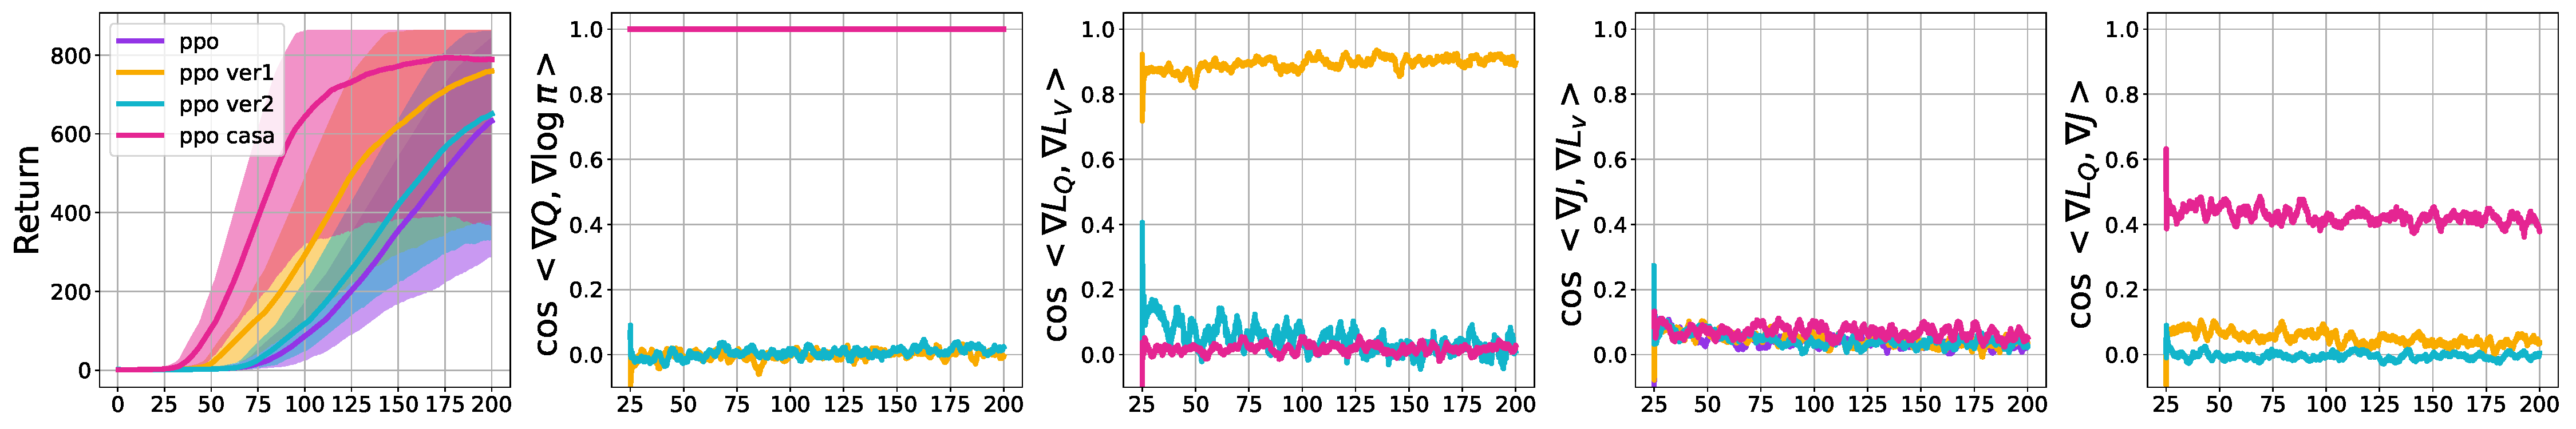
\includegraphics[width=\linewidth]{body/app_fig/app_ppo_Breakout.pdf}

% 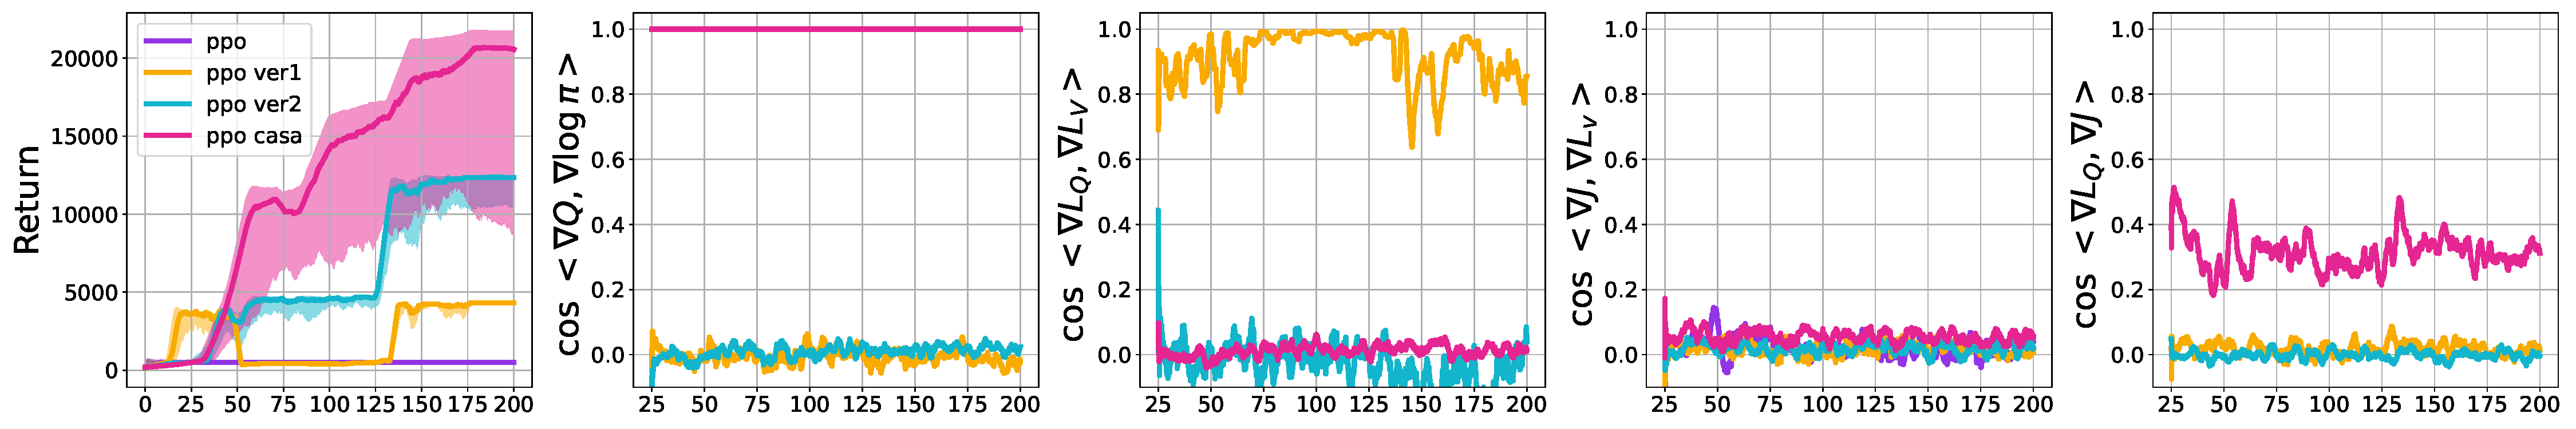
\includegraphics[width=\linewidth]{body/app_fig/app_ppo_Qbert.pdf}

% 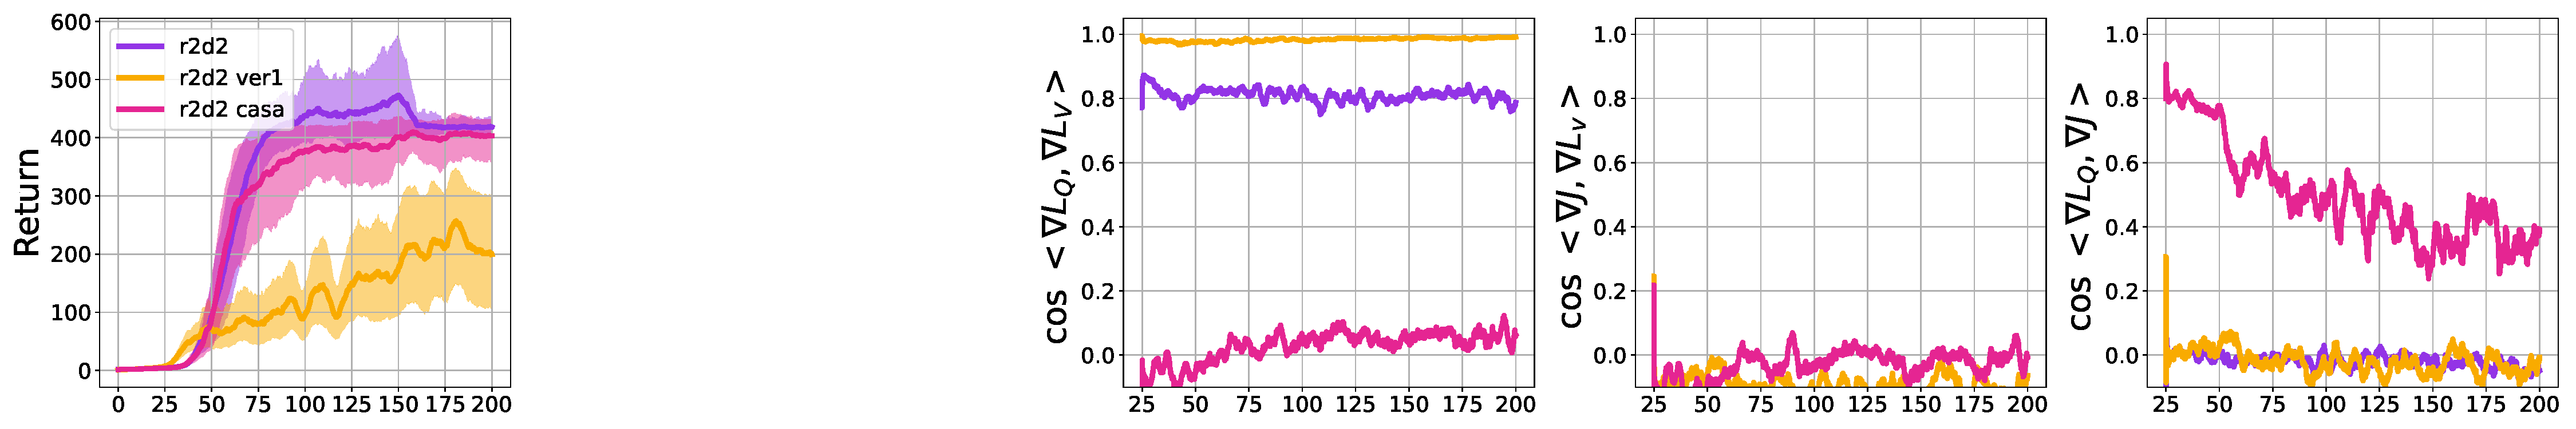
\includegraphics[width=\linewidth]{body/app_fig/app_r2d2_Breakout.pdf}


% 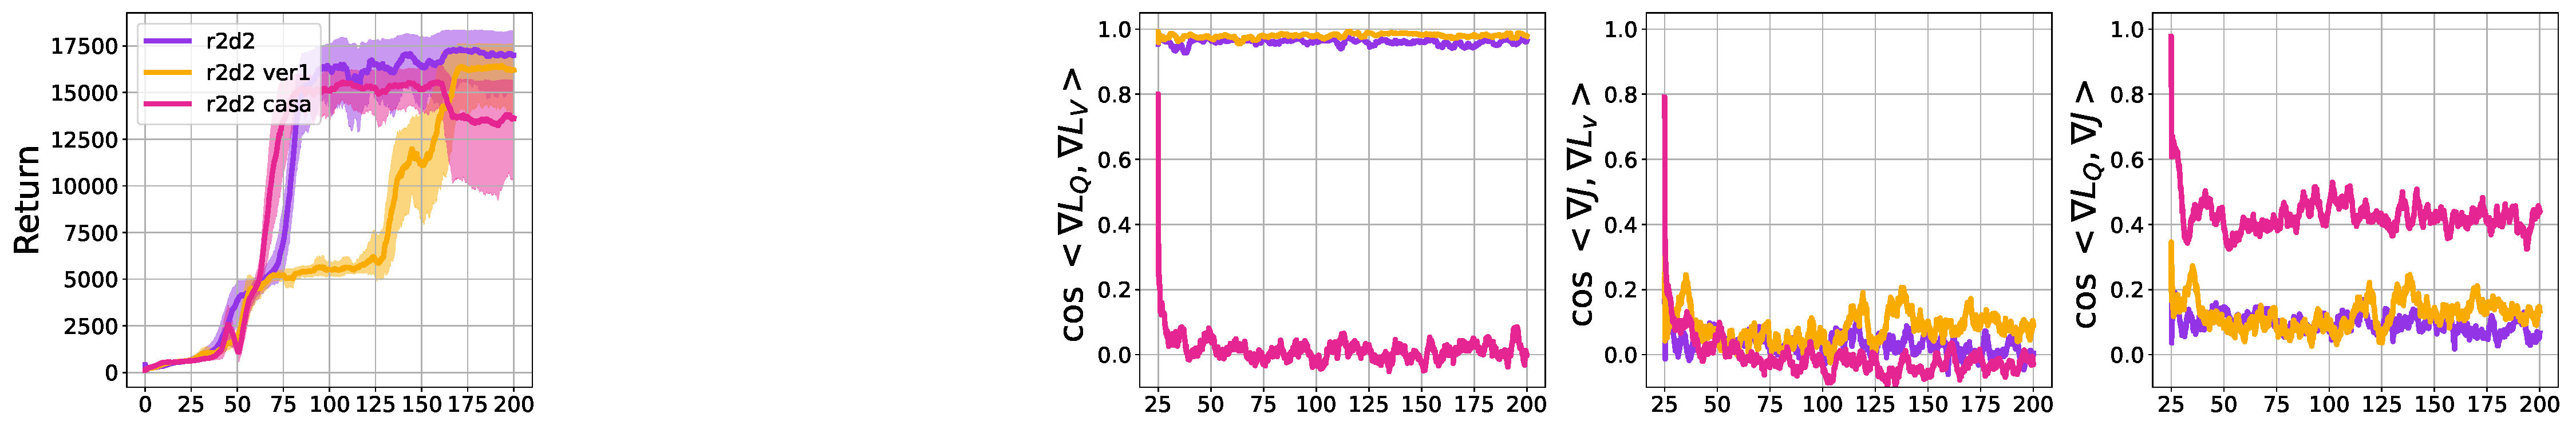
\includegraphics[width=\linewidth]{body/app_fig/app_r2d2_Qbert.pdf}
% \caption{Angles of Gradients and Returns of versions of PPO and R2D2 defined in Table \ref{tab:ppo_mtv} and Table \ref{tab:r2d2_mtv}.}
% \label{fig:mtv_app}
% \end{figure}

% \clearpage

% \changnan{casa summary deleted}
% \section{CASA summary}
% \begin{figure}[ht]
% \centering
% 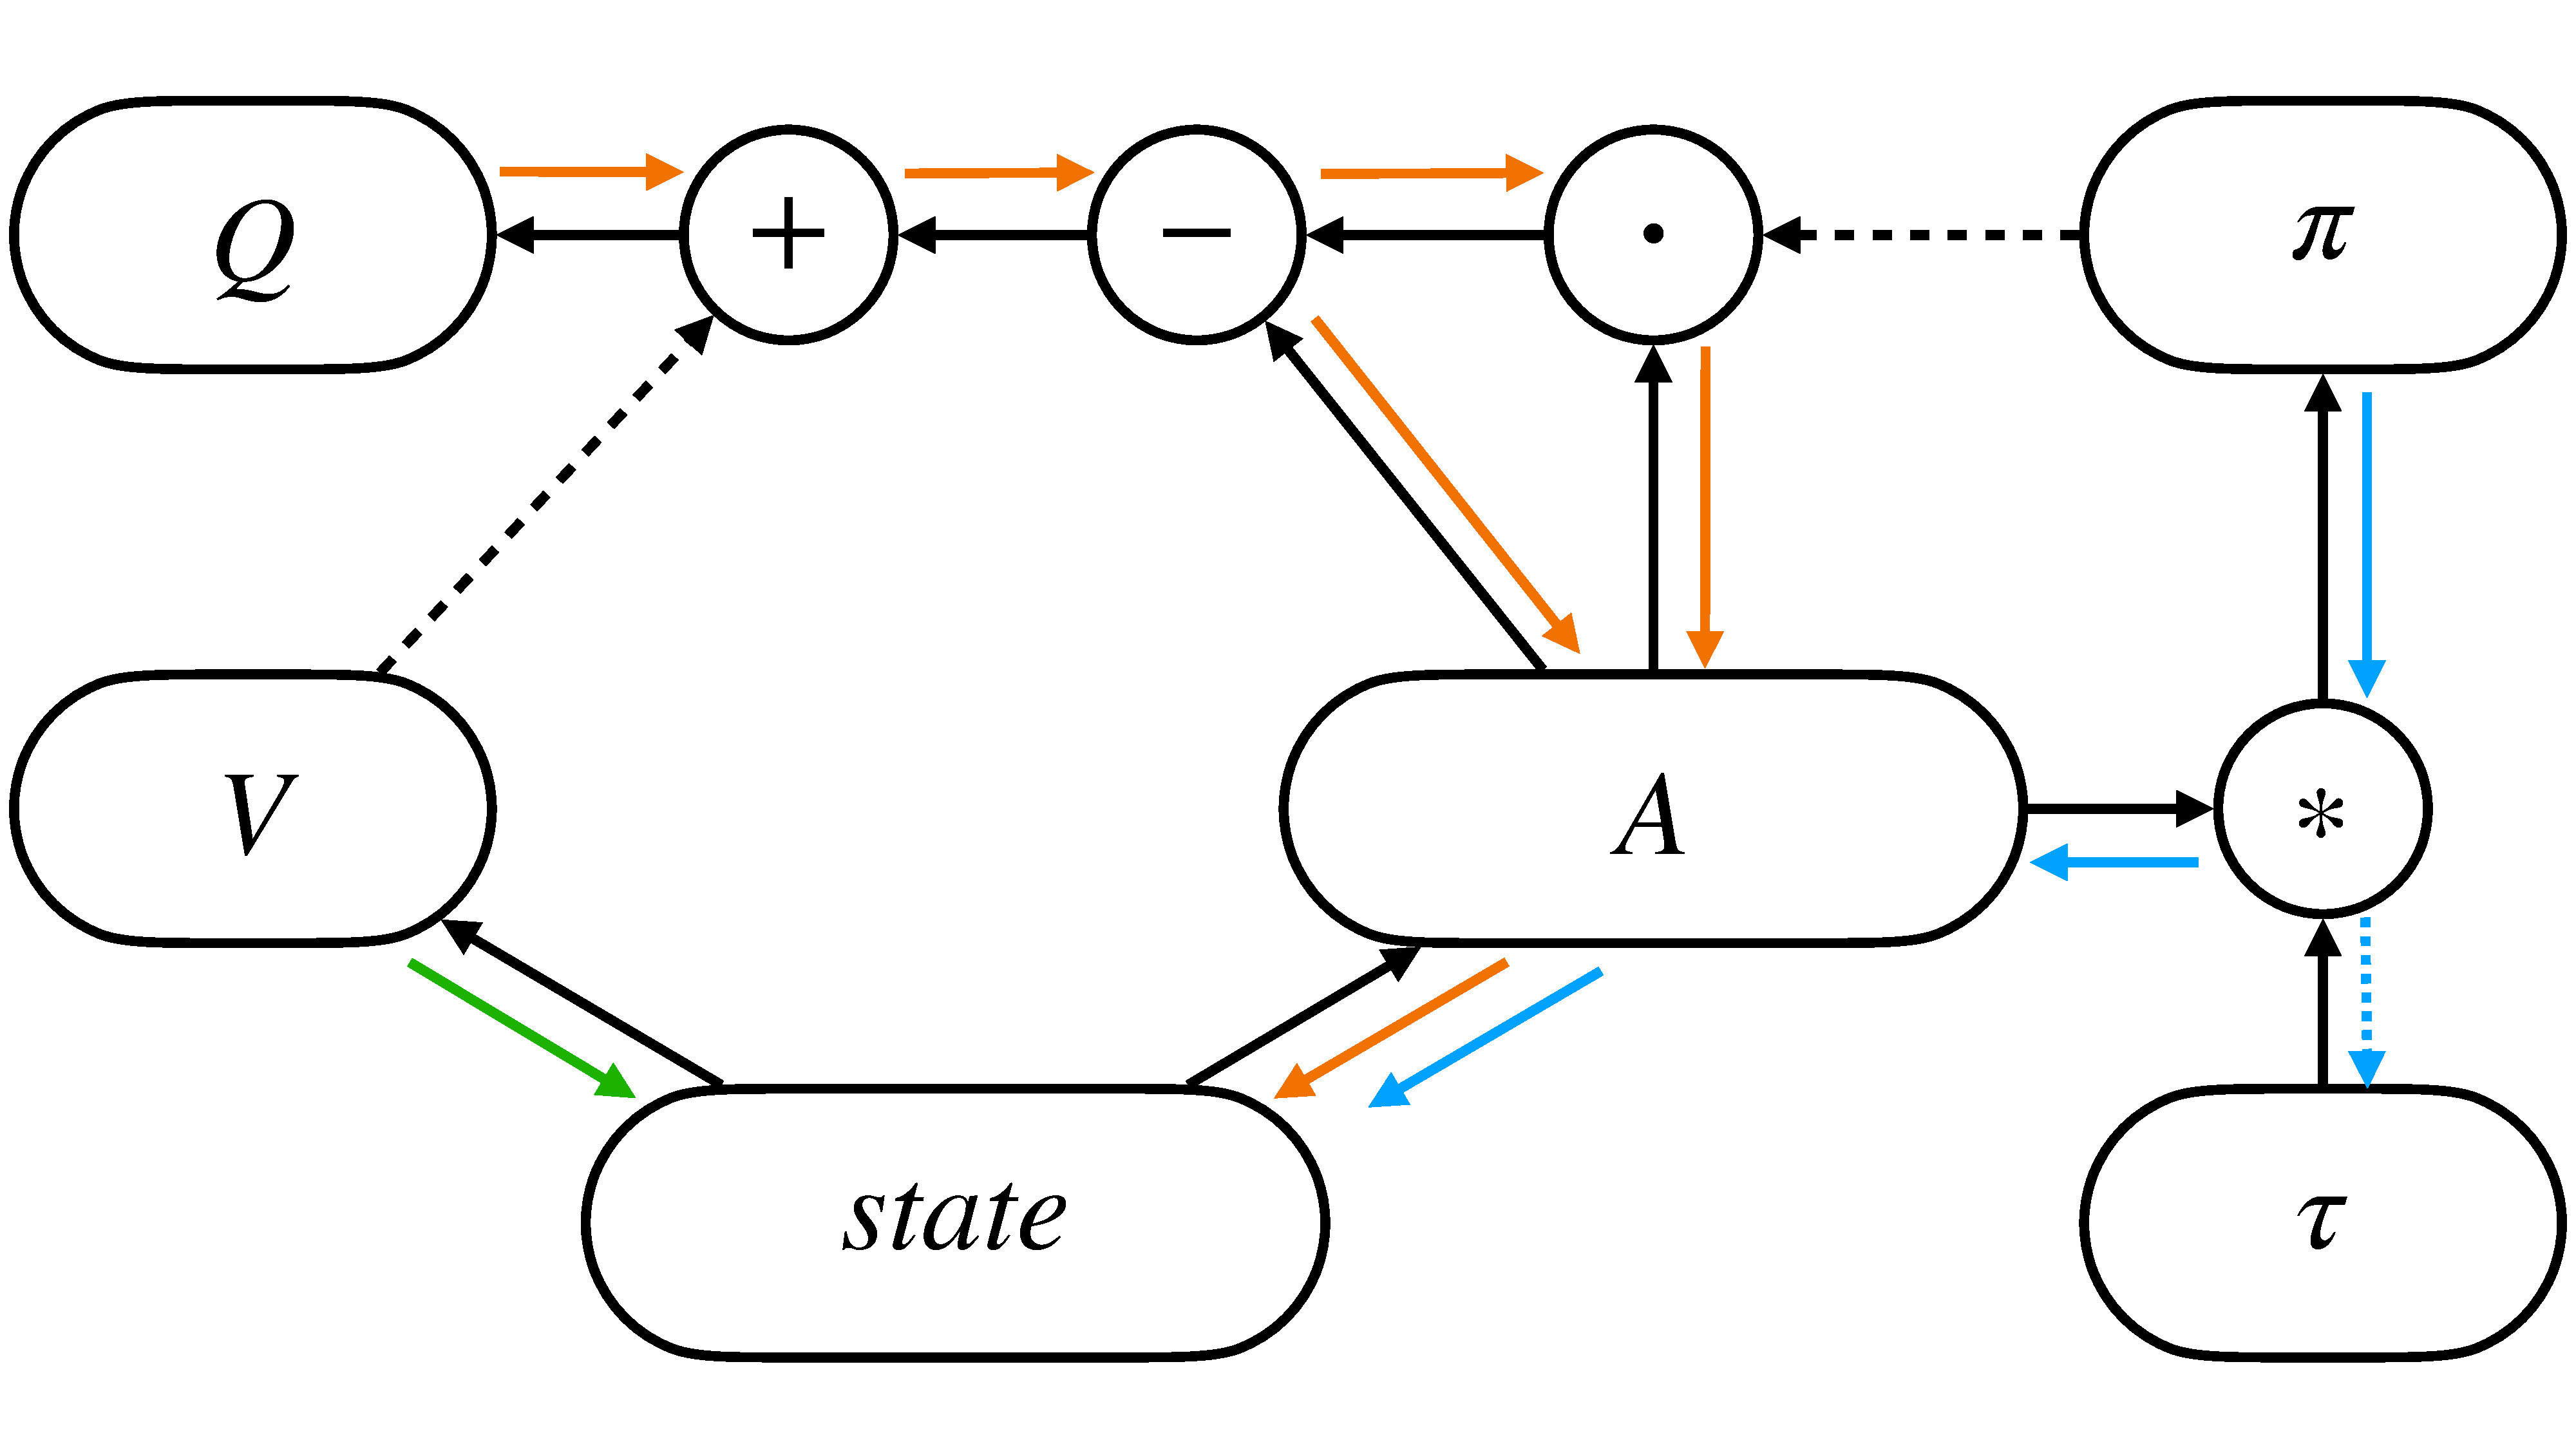
\includegraphics[width=0.4\textwidth,bb= 0 0 1800 1100]{body/figures/CASA.pdf}
% \caption{
% \textbf{Black} lines represent the forward process.
% \textbf{Dotted} black lines represent the \textit{stop gradient} operator in the forward process. 
% \textbf{Colorful} lines represent backpropagation from different loss functions. 
% Specifically, \textbf{blue} lines represent $\mathbb{E}_\pi [(Q^\pi-V)\nabla \log \pi]$, 
% \textbf{orange} lines represent $\mathbb{E}_\pi [(Q^\pi-Q)\nabla Q]$,
% and \textbf{green} lines represent $\mathbb{E}_\pi [(Q^\pi-V)\nabla V]$.}
% \label{fig:casa}
% \end{figure}
% \section{motivation experiments}

\clearpage

{\colorred \section{On Discussing Application of CASA on Continuous Action Space}
\label{app:cts_space}

As we can see CASA is only applied to discrete action space in the main context, we make a discussion on whether CASA is applicable on continuous action space. 
For brevity, we let $\tau=1$ and write \eqref{eq:casa} as:
\begin{equation}
\left\{
    \begin{aligned}
        &\pi = \text{softmax}(A), \\
        &\Bar{A} = A - \mathbb{E}_{\pi} [A], \\
        &Q = \Bar{A} + sg(V).
    \end{aligned}
\right. 
\end{equation}
The difficulty comes from estimating two quantities, one is $\text{softmax}(A)$, the other is $\mathbb{E}_{\pi} [A]$. 
This comes from the fact that discrete action space is countable so these two quantities are expressed in a closed-form, while continuous action space is uncountable so an accurate estimation of these two quantities is intractable. 
We can surely apply Monte Carlo methods to approximate, but a more elegant close-form expression may be preferred. 
Then this becomes another problem: \textit{how to estimate (state-action values / advantages / policy probabilities) of all actions in a continuous action space efficiently without loss of generality?}
This is another representational design problem, which is out of scope of this paper, so we don't touch much about it. 
But with the hope of inspiring a better solution to this problem, we provide one practical way of applying CASA on continuous action space based on kernel-based machine learning. 

Let $a_0, \dots, a_k$ to be basis actions in the action space. 
Let $A(s, a_0), \dots, A(s, a_k)$ to be advantage functions for tuples of states and basis actions. 
They can either share parameters or be isolated. 
Let $K(\cdot, \cdot)$ be a kernel function defined on the product of two action spaces. 
For any $a$ in the action space, we can estimate $A(s, a)$ by a decomposition such like $$A(s, a) = \frac{1}{Z_a} (K(a_0, a) A(s, a_0) + \dots + K(a_k, a) A(s, a_k)),$$ where $Z_a = \sum_{i=0}^k K(a_i, a)$ is a normalization constant. 

Since $K(\cdot, a)$ is a closed-form function of $a$, and $|\{A(s, a_0), \dots, A(s, a_k)\}|$ is finite, we can make a closed-form expression of both $\text{softmax}(A)$ and $\mathbb{E}_{\pi} [A]$. 
Then we can apply CASA directly on this expression, with one function estimates $V$ and the other function estimates advantages of all actions in a closed-form with only state as input.  
The policy is defined directly by $\text{softmax}$ of all advantages. 
In details, we define
\begin{equation}
\left\{
    \begin{aligned}
        &\pi(s, a) = \exp (A(s, a)) / \int_{a} \exp (A(s, a)) da, \\
        &\Bar{A}(s, a) = A(s, a) - \int_{a} sg(\pi(s, a)) A(s, a) da, \\
        &Q(s, a) = \Bar{A}(s, a) + sg(V(s)).
    \end{aligned}
\right. 
\end{equation}

Then it satisfies the consistency of CASA on continuous action space.
$$
\begin{aligned}
    \nabla \log \pi(s, a) &= \nabla A(s, a) - \frac{\nabla \int_{a} \exp (A(s, a)) da}{\int_{a} \exp (A(s, a)) da} \\
    &= \nabla A(s, a) - \frac{ \int_{a} \exp (A(s, a)) \nabla A(s, a) da}{\int_{a} \exp (A(s, a)) da} \\
    &= \nabla A(s, a) - \int_{a} \frac{  \exp (A(s, a)) }{\int_{a} \exp (A(s, a)) da} \nabla A(s, a) da \\
    &= \nabla A(s, a) - \int_{a} \pi(s, a) \nabla A(s, a) da \\
    &= \nabla \Bar{A}(s, a) = \nabla Q(s, a). 
\end{aligned}
$$
}

\section{DR-Trace}
\label{app:drtrace}

% One simple choice is to learn $V$ and $\pi$ by V-Trace \citep{impala} and to learn $Q$ by ReTrace \citep{retrace}. 
% \citep{impala} shows that $V^{\Tilde{\pi}}$ estimated by V-Trace converges to $V^*$ that corresponds to some $\Tilde{\pi}_{VTrace}$.
% Respectively, \citep{retrace} shows that $Q^{\Tilde{\pi}}$ estimated by ReTrace converges to $Q^*$ that corresponds to some $\Tilde{\pi}_{ReTrace}$.

As CASA estimates $(V, Q, \pi)$, we would ask
\textbf{i)} how to guarantee that $\Tilde{\pi}_{VTrace} = \Tilde{\pi}_{ReTrace}$, 
\textbf{ii)} how to exploit $(V, Q, \pi)$ to make a better estimation. 
Though we can apply V-Trace to estimate $V$ and ReTrace to estimate $Q$ with proper hyperparameters to guarantee $\Tilde{\pi}_{VTrace} = \Tilde{\pi}_{ReTrace}$, it's more reasonable to estimate $(V, Q)$ together. 
Inspired by Doubly Robust, which is shown to maximally reduce the variance, we introduce DR-Trace, which estimates $V$ by 
$$
\label{eq:dr-v}
    \begin{aligned}
        V_{DR}^{\Tilde{\pi}} (s_t) &\overset{def}{=} \mathbb{E}_{\mu} [ 
        V(s_t) + \sum_{k \geq 0} \gamma^k 
     c_{[t:t+k-1]} \rho_{t+k}  \delta^{DR}_{t+k} ],  
    \end{aligned}
$$
{\colorred where $\mu$ is the behavior policy}, $\delta^{DR}_t \overset{def}{=} r_t + \gamma V(s_{t+1}) - Q(s_t, a_t)$ is one-step Doubly Robust error, $\rho_t \overset{def}{=} \min\{\frac{\pi_t}{\mu_t}, \Bar{\rho} \}$ and $c_t \overset{def}{=} \min\{\frac{\pi_t}{\mu_t}, \Bar{c}\}$ are clipped per-step importance sampling, $c_{[t: t+k]} \overset{def}{=} \prod_{i=0}^{k} c_{t+i}$.

With one step Bellman equation, we estimate $Q$ by
$$
\label{eq:dr-q}
    \begin{aligned}
         Q_{DR}^{\Tilde{\pi}} (s_t, a_t) 
         &\overset{def}{=} \mathbb{E}_{s_{t+1}, r_t \sim p(\cdot, \cdot | s_t, a_t)} [  r_t + \gamma   V_{DR}^{\Tilde{\pi}} (s_{t+1}) ] 
        \\
        %  &=  \mathbb{E}_{\mu} [ r_t + \gamma V(s_{t + 1}) +
        % \gamma \sum_{k \geq 0} \gamma^k 
        % c_{[t+1:t+k]} \rho_{t+1+k}
        % \delta^{DR}_{t+1+k} V
        % ]
        % \\
        %  &= \mathbb{E}_{\mu}   [
        % Q(s_t, a_t) + \delta_t^{DR}V + \sum_{k \geq 1}  \gamma^k
        % c_{[t+1:t+k-1]} \rho_{t+k}
        % \delta^{DR}_{t+k} V
        % ],
        % \\
        &=  \mathbb{E}_{\mu}   [
        Q(s_t, a_t) + \sum_{k \geq 0}  \gamma^k
        c_{[t+1:t+k-1]} \Tilde{\rho}_{t, k}
        \delta^{DR}_{t+k}
        ], 
    \end{aligned}
$$
where $\Tilde{\rho}_{t, k} =  1_{\{k=0\}} + 1_{\{k > 0\}} \rho_{t+k}$.

% Compared to \eqref{eq:dr-v}, $c_{[t+1:t+k-1]} \Tilde{\rho}_{t, k}$ in \eqref{eq:dr-q} doesn't multiply importance sampling ratio of $a_t$, which meets the same intuition as \eqref{eq:vtrace} and \eqref{eq:retrace}.\\
\begin{theorem}
    Define $\Bar{A} = A - \mathbb{E}_\pi[A]$, $Q = \Bar{A} + sg(V)$,
    $$
    \begin{aligned}
    &\mathscr{T}(Q) \overset{def}{=} \mathbb{E}_{\mu}   [
        Q(s_t, a_t) + \sum_{k \geq 0}  \gamma^k
        c_{[t+1:t+k-1]} \Tilde{\rho}_{t, k}
        \delta^{DR}_{t+k}
        ], \\
    &\mathscr{S}(V) \overset{def}{=} \mathbb{E}_{\mu}   [
        V(s_t) + \sum_{k \geq 0}  \gamma^k
        c_{[t:t+k-1]} \rho_{t, k}
        \delta^{DR}_{t+k}
        ], \\
    &\mathscr{U}(Q, V) = (\mathscr{T}(Q) - \mathbb{E}_\pi[Q] + \mathscr{S}(V), \mathscr{S}(V)), \\
    &\mathscr{U}^{(n)}(Q, V) = \mathscr{U}(\mathscr{U}^{(n-1)}(Q, V)),
    \end{aligned}
    $$
    then $\mathscr{U}^{(n)}(Q, V) \rightarrow (Q^{\Tilde{\pi}}, V^{\Tilde{\pi}})$ that corresponds to 
    $$
        \Tilde{\pi}(a|s) = \frac
        {\min \left\{\Bar{\rho} \mu (a|s), \pi(a|s)\right\}}
        {\sum_{b \in \mathcal{A}}\min \left\{\Bar{\rho} \mu (b|s), \pi(b|s)\right\}}.
    $$ as $n \rightarrow +\infty$.
\label{thm:dr}
\end{theorem}
\begin{proof}
    See Appendix \ref{app:proof}, Theorem \ref{thm_app:dr}.
\end{proof}
Theorem \ref{thm:dr} shows that DR-Trace is a contraction mapping and $(V, Q)$ converges to $(V^{\Tilde{\pi}}, Q^{\Tilde{\pi}})$ that corresponds to 
$$
    \begin{aligned}
        \Tilde{\pi}(a|s) = \frac
        {\min \left\{\Bar{\rho} \mu (a|s), \pi(a|s)\right\}}
        {\sum_{b \in \mathcal{A}}\min \left\{\Bar{\rho} \mu (b|s), \pi(b|s)\right\}}.
    \end{aligned}
$$

% At training time, the policy evaluation is achieved by updating $\theta$ to minimize $l2$ losses
% $$
% \begin{aligned}
%     L_V(\theta) &= \mathbb{E}_\pi [ (V_\theta(s_t) -  V_{DR}^{\Tilde{\pi}} (s_t))^2 ], \\
%     L_Q(\theta) &= \mathbb{E}_\pi [ (Q_\theta(s_t, a_t) -  Q_{DR}^{\Tilde{\pi}} (s_t, a_t))^2 ],
% \end{aligned}
% $$ 
% which gives the ascent direction of $\theta$ by
% \begin{equation}
% \label{eq:grad_qv}
%     \begin{aligned}
%         \nabla_\theta L_V(\theta)
%         &= \mathbb{E}_\pi \left[ (V_{DR}^{\Tilde{\pi}} (s_t) - V_\theta(s_t) ) \nabla V_\theta(s_t) \right], \\
%         \nabla_\theta L_Q(\theta)
%         &= \mathbb{E}_\pi \left[ (Q_{DR}^{\Tilde{\pi}} (s_t, a_t) - Q_\theta(s_t, a_t)) \nabla Q_\theta(s_t, a_t) \right].
%     \end{aligned}
% \end{equation}
% And we make the policy improvement by policy gradient, which gives the ascent direction of $\theta$ by 
% \begin{equation}
% \label{eq:grad_pi}
% \begin{aligned}
%     \nabla_\theta \mathcal{J}(\tau, \theta) = \mathbb{E}_\mu \left[\tau \rho_t (Q_{DR}^{\Tilde{\pi}} (s_t, a_t) - V_\theta(s_t) ) \nabla_\theta \log \pi_t \right],
% \end{aligned}
% \end{equation}
% where $\mathcal{J} (\tau, \theta) = \tau \mathbb{E}_\pi [\sum \gamma^t r_t]$.
% It takes an additional $\tau$, which frees the scale of gradient from $\tau$.

% Finally, the gradient ascent direction of $\theta$ is given by
% \begin{equation}
%     \label{eq:grad_all}
%     \alpha_1 \nabla_\theta L_V + \alpha_2 \nabla_\theta L_Q + \alpha_3 \nabla_\theta \mathcal{J}.
% \end{equation}

% \textbf{Full algorithm is described in Appendix \ref{app:casa}.}
% Note that \eqref{eq:grad_all} doesn't need any entropy regularization. 
% We will discuss why this happens in section \ref{sec:equiv} and how CASA controls the exploration in section \ref{sec:ent_control}.


\begin{figure}[h]
    \centering
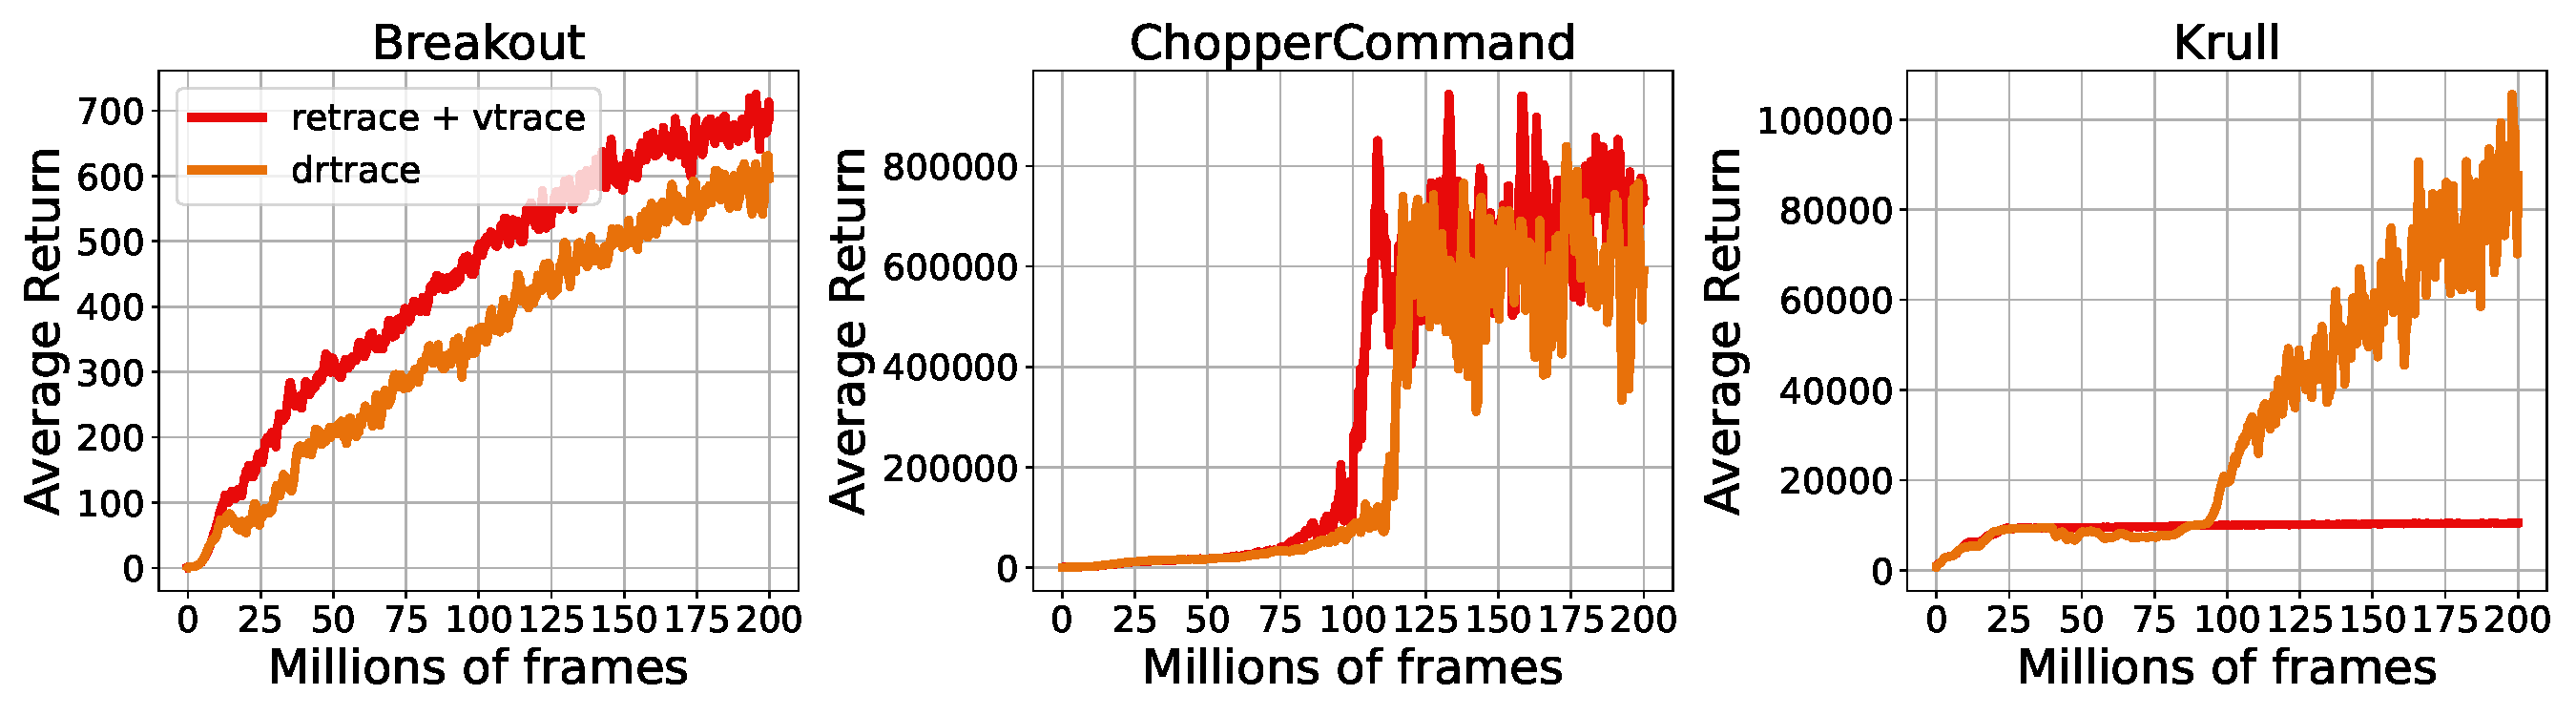
\includegraphics[width=\linewidth]{body/ablation/dr_ablation.pdf}
    \caption{Ablation study for w/wo DR-Trace on Breakout, ChopperCommand and Krull.}
    \label{fig:app_dr_trace}
\end{figure}

According to our proof, DR-Trace should work similar to V-Trace and ReTrace, as the convergence rate and the limitation are same. 
We compare DR-Trace with V-Trace+ReTrace in Figure \ref{fig:app_dr_trace}, where we replace estimation of state values by V-Trace and estimation of state-action values by ReTrace. 
We call V-Trace+ReTrace as No-DR-Trace for brevity. 
No-DR-Trace performs better on Breakout and ChopperCommand, but fails to make a breakthrough on Krull. 
Recalling the fact that Doubly Robust can maximally reduce the variance of Bellman error, No-DR-Trace is less stable but also potential to achieve a better performance. 
A conclusion cannot be made about No-DR-Trace, as this phenomenon means that No-DR-Trace is less stable than DR-Trace, but it also holds the potential to achieve a better performance.

% \clearpage


\section{Proofs}
\label{app:proof}

\theoremstyle{plain}
% \setcounter{Lemma}{0}
\newtheorem{Lemma_app}{Lemma}[section]
\newtheorem{Theorem_app}{Theorem}[section]
\theoremstyle{definition}
\newtheorem*{Remark_app}{Remark}
\theoremstyle{remark}

% \begin{Lemma_app}
% Let 
% $g \in \textbf{C}^{1}(\mathbb{R}^{n}): \mathbb{R}^{n} \to \mathbb{R}^{n}, \ f \in \textbf{C}^{1}(\mathbb{R}^{n+k}): \mathbb{R}^{n+k} \to \mathbb{R}^{n}.
% $\\
% If
% $
% \nabla_x g(x) = \nabla_x f(x, y)$, for $\forall x\in \mathbb{R}^{n}, y\in \mathbb{R}^k,
% $
% then $\exists$ $c \in \textbf{C}^{1}(\mathbb{R}^{k}): \mathbb{R}^{k} \to \mathbb{R}^{n}$, s.t. $f(x, y) = g(x) + c(y)$.
% \label{lemma_app:func_sep}
% \end{Lemma_app}
% \begin{proof}

% Let $\Tilde{f}(x, y) = f(x, y) - g(x)$.

% Since $\nabla_x g(x) = \nabla_x f(x, y)$, we have 
% $$
% \nabla_x \Tilde{f} = 0, \ for \ \forall x\in \mathbb{R}^{n}, y\in \mathbb{R}^k.
% $$

% So $\Tilde{f}$ is a constant function w.r.t $x$, which can be denoted as $c(y) = \Tilde{f}(x, y)$.

% Hence, $f(x, y) = g(x) + c(y)$.
% \end{proof}

\begin{Lemma_app}
(i) Define $\pi = softmax(A / \tau)$, then $\nabla \log \pi = (\textbf{1} - \pi) \frac{\nabla A}{\tau}$. 
(ii) Denote $sg$ to be stop gradient and define $\Bar{A} = A - \mathbb{E}_\pi [A]$, $Q = \Bar{A} + sg(V)$, then $\nabla Q = (\textbf{1} - \pi) \nabla A$.
\label{lemma_app:vannila_grad}
\end{Lemma_app}
\begin{proof}

As $Q = \Bar{A} + sg(V) = A - sg(\pi)\cdot A + sg(V)$, it's obvious that $\nabla Q = (\textbf{1} - \pi) \nabla A$.

For $\log \pi$, it's a standard derivative of cross entropy, so we have $\nabla \log \pi = (\textbf{1} - \pi) \nabla (A / \tau) = (\textbf{1} - \pi) \frac{\nabla A}{\tau}$.
\end{proof}

\begin{Lemma_app}
Define $\Bar{A}= A - \mathbb{E}_\pi[A]$, $Q = \Bar{A} + sg(V), \pi = softmax(A / \tau)$, then 
$$
\mathbb{E}_\pi \left[ (Q - V) \nabla \log \pi \right]
= - \tau \nabla \textbf{H}[\pi].
$$
\label{lemma_app:eqiv_pg_ent}
\end{Lemma_app}
\begin{proof}
Since 
$$
\pi = \exp(A / \tau) / Z,\ Z = \int_\mathcal{A} \exp(A / \tau),
$$
we have 
$$
A = \tau \log \pi + \tau \log Z.
$$
Based on the observation that $\mathbb{E}_\pi \left[ f(s) \nabla \log \pi (\cdot | s) \right] = 0$, 
we have 
$$\mathbb{E}_\pi \left[ \mathbb{E}_\pi[A] \cdot \nabla \log \pi \right] = 0,$$ 
$$\mathbb{E}_\pi \left[ \log Z \cdot \nabla \log \pi \right] = 0.$$

On the one hand,
$$
\begin{aligned}
    \mathbb{E}_\pi \left[ (Q - V) \nabla \log \pi \right]
    &= \mathbb{E}_\pi \left[ A \nabla \log \pi \right] 
    - \mathbb{E}_\pi \left[ \mathbb{E}_\pi[A] \cdot \nabla \log \pi \right] \\
    &= \tau \mathbb{E}_\pi \left[ \log \pi \nabla \log \pi \right]
    + \tau \mathbb{E}_\pi \left[ \log Z \cdot \nabla \log \pi \right] \\
    &= \tau \mathbb{E}_\pi \left[ \log \pi \nabla \log \pi \right].
\end{aligned}
$$

On the other hand, 
$$
\begin{aligned}
    \nabla \textbf{H} [\pi] 
    &= - \nabla \int_\mathcal{A} \pi_i \log \pi_i \\
    &= - \int_\mathcal{A}  \nabla \pi_i \cdot \log \pi_i - \int_\mathcal{A} \pi_i \nabla \log \pi_i  \\
    &= - \int_\mathcal{A}  \pi_i \nabla \log \pi_i \cdot \log \pi_i - \int_\mathcal{A}  \pi_i \frac{\nabla \pi_i}{\pi_i} \\
    &= - \mathbb{E}_\pi \left[ \log \pi \nabla \log \pi \right].
\end{aligned}
$$
Hence, $
\mathbb{E}_\pi \left[ (Q - V) \nabla \log \pi \right]
= - \tau \nabla \textbf{H}[\pi]
$.
\end{proof}

\begin{Theorem_app}
    Define $\Bar{A} = A - \mathbb{E}_\pi[A]$, $Q = \Bar{A} + sg(V)$.
    Define $$
    \begin{aligned}
    &\mathscr{T}(Q) \overset{def}{=} \mathbb{E}_{\mu}   [
        Q(s_t, a_t) + \sum_{k \geq 0}  \gamma^k
        c_{[t+1:t+k-1]} \Tilde{\rho}_{t, k}
        \delta^{DR}_{t+k}
        ], \\
    &\mathscr{S}(V) \overset{def}{=} \mathbb{E}_{\mu}   [
        V(s_t) + \sum_{k \geq 0}  \gamma^k
        c_{[t:t+k-1]} \rho_{t, k}
        \delta^{DR}_{t+k}
        ], \\
    &\mathscr{U}(Q, V) = (\mathscr{T}(Q) - \mathbb{E}_\pi[Q] + \mathscr{S}(V), \mathscr{S}(V)), \\
    &\mathscr{U}^{(n)}(Q, V) = \mathscr{U}(\mathscr{U}^{(n-1)}(Q, V)),
    \end{aligned}
    $$
    then $\mathscr{U}^{(n)}(Q, V) \rightarrow (Q^{\Tilde{\pi}}, V^{\Tilde{\pi}})$ that corresponds to 
    $$
        \Tilde{\pi}(a|s) = \frac
        {\min \left\{\Bar{\rho} \mu (a|s), \pi(a|s)\right\}}
        {\sum_{b \in \mathcal{A}}\min \left\{\Bar{\rho} \mu (b|s), \pi(b|s)\right\}}.
    $$ as $n \rightarrow +\infty$.
\label{thm_app:dr}
\end{Theorem_app}
\begin{Remark_app}
$\mathscr{T}(Q) - \mathbb{E}_\pi[Q] + \mathscr{S}(V)$ is \textbf{exactly} how $Q$ is updated at training time. 
Since $Q = \Bar{A} + sg(V)$, if we apply gradient ascent on $Q$ and $V$ in directions $\nabla L_Q(\theta)$ and $\nabla L_V(\theta)$ respectively, change of $Q$ comes from two aspects. One comes from $\nabla L_Q(\theta)$, which changes $A$, the other comes from $\nabla L_V(\theta)$, which changes $V$. Because the gradient of $V$ is stopped when estimating $Q$, the latter is captured by "minus old baseline, add new baseline", which is $- \mathbb{E}_\pi[Q] + \mathscr{S}(V)$ in Theorem \ref{thm_app:dr}.
\end{Remark_app}
\begin{proof}
 Define
 $$
 \begin{aligned}
        \widetilde{\mathscr{T}}(Q) &= - \mathbb{E}_\pi[Q] + \mathscr{T}(Q), \\
        \widetilde{\mathscr{U}}(Q, V) &= (\widetilde{\mathscr{T}}(Q), \mathscr{S}(V)), \\
        \widetilde{\mathscr{U}}^{(n)}(Q, V) &=   \widetilde{\mathscr{U}}(\widetilde{\mathscr{U}}^{(n-1)}(Q, V)).
 \end{aligned}
 $$
By Lemma \ref{lemma_app:dr_q}, $\widetilde{\mathscr{T}}^{(n)}(Q)$ converges to some $A^*$ as $n \rightarrow \infty$. This process will not influence the estimation of $V$ as the gradient of $V$ is stopped when estimating $Q$. According to the proof, $A^*$ does not depend on $V$. \\
By Lemma \ref{lemma_app:dr_v}, $\mathscr{S}^{(n)}(V)$ converges to some $V^*$ as $n \rightarrow \infty$. \\
Hence, we have
$$
\widetilde{\mathscr{U}}^{(n)}(Q, V) \rightarrow (A^*, V^*)\ \ as\ \ n \rightarrow +\infty. 
$$
By definition, 
$$
\mathscr{U}(Q, V) = (\widetilde{\mathscr{T}}(Q) + \mathscr{S}(V), \mathscr{S}(V)),
$$
we can regard $\widetilde{\mathscr{T}}(Q) + \mathscr{S}(V)$ as $Q$ and regard $\mathscr{S}(V)$ as $V$, then
$$
\begin{aligned}
    \mathscr{U}^{(2)}(Q, V) 
    &= \mathscr{U}(\widetilde{\mathscr{T}}(Q) + \mathscr{S}(V), \mathscr{S}(V)) \\
    &= (\mathscr{T}(\widetilde{\mathscr{T}}(Q) + \mathscr{S}(V)) -\mathscr{S}(V) + \mathscr{S}^{(2)}(V), \mathscr{S}^{(2)}(V)) \\
    &= (\widetilde{\mathscr{T}}^{(2)}(Q) + \mathscr{S}^{(2)}(V), \mathscr{S}^{(2)}(V)).
\end{aligned}
$$
By induction, 
$$
\begin{aligned}
    \mathscr{U}^{(n)}(Q, V) &= (\widetilde{\mathscr{T}}^{(n)}(Q) + \mathscr{S}^{(n)}(V), \mathscr{S}^{(n)}(V)) \\
    &\rightarrow (A^*+V^*, V^*)\ \ as\ \ n\rightarrow + \infty.
\end{aligned}
$$
Same as \citep{impala}, 
$$
    \Tilde{\pi}(a|s) = \frac
    {\min \left\{\Bar{\rho} \mu (a|s), \pi(a|s)\right\}}
    {\sum_{b \in \mathcal{A}}\min \left\{\Bar{\rho} \mu (b|s), \pi(b|s)\right\}}.
$$ 
is the policy s.t. the Bellman equation holds, which is 
$$\mathbb{E}_\mu[\rho_t (r_t + \gamma V_{t+1} - V_t) | \mathscr{F}_t] = 0,$$ and $\mathscr{U}(Q^{\Tilde{\pi}}, V^{\Tilde{\pi}}) = (Q^{\Tilde{\pi}}, V^{\Tilde{\pi}})$. \\
So we have
$(A^*+V^*, V^*) = (Q^{\Tilde{\pi}}, V^{\Tilde{\pi}}).$
\end{proof}

\begin{Lemma_app}
Define $\Bar{A}= A - \mathbb{E}_\pi[A]$, $Q = \Bar{A} + sg(V)$,
then operator 
$$
    \mathscr{T}(Q) \overset{def}{=} \mathbb{E}_{\mu}   [
        Q(s_t, a_t) + \sum_{k \geq 0}  \gamma^k
        c_{[t+1:t+k-1]} \Tilde{\rho}_{t, k}
        \delta^{DR}_{t+k}
        ]
$$
is a contraction mapping w.r.t. $Q$.
\label{lemma_app:dr_q}
\end{Lemma_app}
\begin{Remark_app}
Note that $\mathscr{T}(Q)$ is exactly \eqref{eq:dr-q}. 

Since $Q = A + sg(V)$, the gradient of $V$ is stopped when estimating $Q$, updating $Q$ will not change $V$, which is equivalent to updating $A$.
Without loss of generality, we assume $V$ is fixed as $V^*$ in the proof.
\end{Remark_app}
\begin{proof}

$\Bar{A} = A - \mathbb{E}_\pi[A]$ shows $\mathbb{E}_\pi[\Bar{A}] = 0$, which guarantees that no matter how we update $A$, we always have $\mathbb{E}_\pi[Q] = V^*$.

Based on above observations, define 
$$
    \widetilde{\mathscr{T}}(Q) \overset{def}{=} - \mathbb{E}_\pi [Q] + \mathscr{T}(Q).
$$

It's obvious that we only need to prove $\widetilde{\mathscr{T}}(Q)$ is a contraction mapping.

For brevity, we denote $$Q_t = Q(s_t, a_t), A_t = A(s_t, a_t), V^*_t = V^*(s_t).$$

Noticing that $\Tilde{\rho}_{t, 0} = 1$, let $\mathscr{F}$ represent filtration, we can rewrite $\widetilde{\mathscr{T}}$ as 
\begin{equation}
\label{eq:dr_a_2}
\begin{aligned}
    \widetilde{\mathscr{T}}(Q)
    &= \mathbb{E}_{\mu}   [
        A_t + \sum_{k \geq 0}  \gamma^k
        c_{[t+1:t+k-1]} \Tilde{\rho}_{t, k}
        \delta^{DR}_{t+k}
        ] \\
    &= \mathbb{E}_{\mu}   [
        -V^*_t + \sum_{k \geq 0}  \gamma^k
        c_{[t+1:t+k-1]} \Tilde{\rho}_{t, k}
        r_{t+k}
        + 
        \sum_{k \geq 0}  \gamma^{k+1}
        c_{[t+1:t+k-1]} \Delta_k ],
        \\
\end{aligned}
\end{equation}
where 
\begin{equation}
\label{eq:dr_delta}
    \Delta_k = \mathbb{E}_{\mu}\left[\Tilde{\rho}_{t, k} V^*_{t+k+1} - c_{t+k} \Tilde{\rho}_{t, k+1} Q_{t+k+1} | \mathscr{F}_{t+k}\right].
\end{equation}
By definition of $Q$,
$$
    \mathbb{E}_{\mu}[V_{t+k+1}^*|\mathscr{F}_{t+k}] 
    = \mathbb{E}_{\mu}[
    \mathbb{E}_\pi[Q_{t+k+1}|\mathscr{F}_{t+k+1}]
    |\mathscr{F}_{t+k}], \\
    % \geq&  \mathbb{E}_{\mu}[
    % \mathbb{E}_\mu[\Tilde{\rho}_{t, k+1} Q_{t+k+1}|\mathscr{F}_{t+k+1}]
    % |\mathscr{F}_{t+k}], 
$$
we can rewrite \eqref{eq:dr_delta} as
\begin{equation}
\label{eq:dr_q_delta}
\Delta_k = \mathbb{E}_{\mu}[
(
\Tilde{\rho}_{t, k} \frac{\pi_{t+k+1}}{\mu_{t+k+1}}- c_{t+k} \Tilde{\rho}_{t, k+1} 
) Q_{t+k+1} | \mathscr{F}_{t+k}
].
\end{equation}
For any $Q_1 = A_1 + sg(V^*)$, $Q_2 = A_2 + sg(V^*)$, since
$$
\mathbb{E}_{\mu}[
(
\Tilde{\rho}_{t, k} \frac{\pi_{t+k+1}}{\mu_{t+k+1}}- c_{t+k} \Tilde{\rho}_{t, k+1} 
) | \mathscr{F}_{t+k}
] \geq 0,
$$
by \eqref{eq:dr_a_2} \eqref{eq:dr_q_delta}, we have 
% $$
% || \Delta^1_k - \Delta_k^2 || \leq \mathbb{E}_{\mu}\left[
% \left(
% \Tilde{\rho}_{t, k} \frac{\pi_{t+k+1}}{\mu_{t+k+1}}- c_{t+k} \Tilde{\rho}_{t, k+1} 
% \right) | \mathscr{F}_{t+k}
% \right] ||A^1 - A_2||.
% $$
$$
        || \widetilde{\mathscr{T}}(Q_1) - \widetilde{\mathscr{T}}(Q_2) || 
        % \leq& \mathbb{E}_{\mu} \left[ \sum_{k \geq 0}  \gamma^{k+1} c_{[t+1:t+k-1]} || \Delta_k^1 - \Delta_k^2 || \right] \\
        \leq \mathcal{C} || Q_1 - Q_2 ||,
$$
where 
$$
    \begin{aligned}
        \mathcal{C} 
        &= \mathbb{E}_{\mu} [ \sum_{k \geq 0}  \gamma^{k+1} c_{[t+1:t+k-1]} 
        (
        \Tilde{\rho}_{t, k} \frac{\pi_{t+k+1}}{\mu_{t+k+1}}- c_{t+k} \Tilde{\rho}_{t, k+1} 
        ) ]
        \\
        &= \mathbb{E}_{\mu} [1 -1 + \sum_{k \geq 0}  \gamma^{k+1} c_{[t+1:t+k-1]} 
        \left(
        \Tilde{\rho}_{t, k} - c_{t+k} \Tilde{\rho}_{t, k+1} 
        \right) ] 
        \\
        &= 1 - (1 - \gamma)  \mathbb{E}_{\mu} [\sum_{k \geq 0} \gamma^{k}c_{[t+1:t+k-1]} \Tilde{\rho}_{t, k}  ] \\
        &\leq 1 - (1 - \gamma) < 1.
    \end{aligned}
$$
Hence, $\widetilde{\mathscr{T}}(Q)$ is a contraction mapping and converges to some fixed function, which we denote as $A^*$. So $\mathscr{T}(Q)$ is also a contraction mapping and converges to $A^*+V^*$.
\end{proof}

\begin{Lemma_app}
Define $Q = A + sg(V)$ with $\mathbb{E}_\pi [A] = 0$,
then operator 
$$
    \mathscr{S}(V) \overset{def}{=} \mathbb{E}_{\mu}  [
        V(s_t) + \sum_{k \geq 0}  \gamma^k
        c_{[t:t+k-1]} \rho_{t, k}
        \delta^{DR}_{t+k}
        ]
$$
is a contraction mapping w.r.t. $V$.
\label{lemma_app:dr_v}
\end{Lemma_app}
\begin{Remark_app}
Note that $\mathscr{S}(V)$ is exactly \eqref{eq:dr-v}. 
\end{Remark_app}
\begin{proof}

% Since $Q = A + sg(V)$, updating $V$ wouldn't influence $A$. WLOG, we assume $A$ is fixed as $A^*$ in Lemma \ref{lemma_app:dr_v}. \\
Same as Lemma \ref{lemma_app:dr_q}, we can get
$$
    \Delta_k = \mathbb{E}_{\mu}\left[
    \left( \rho_{t+k} - c_{t+k} \rho_{t+k+1}\right) V_{t+k+1} 
     -  c_{t+k} \rho_{t+k+1} A^*_{t+k+1} | \mathscr{F}_{t+k}\right],
$$
so we have 
$$
    \Delta^1_k - \Delta^2_k = \mathbb{E}_{\mu}\left[ 
    \left( \rho_{t+k} - c_{t+k} \rho_{t+k+1}\right) \cdot  
   (V^1_{t+k+1} -  V^2_{t+k+1})
     | \mathscr{F}_{t+k}\right].
$$
The remaining proof is identical to \citep{impala}'s.
\end{proof}

% \clearpage

% \begin{Lemma_app}
% Let $v \in \mathbb{R}^{|\mathcal{A}|}$ to be a vector. 
% Define 
% $
%     \pi (\tau) = \exp (v / \tau) / Z,\  Z = \int_\mathcal{A}  \exp(v / \tau).
% $
% Let $\Omega$ to be a probability measure supported on $[K, +\infty]$,
% then $f(\Omega) = \mathbb{E}_{\tau \sim \Omega} [\mathbb{E}_{\pi(\tau)} [v]]$ satisfies Lipschitz-1 condition with Wasserstein-1 metric.
% \label{lemma_app:lips}
% \end{Lemma_app}
% \begin{proof}
% Without loss of generality, we assume $v_1 \geq v_2 \geq ... \geq v_{|\mathcal{A}|}$.

% For any $\tau \in [0, +\infty)$, since
% $$
% \begin{aligned}
%     \pi (\tau) = \exp (v / \tau) / Z,\  Z = \int_\mathcal{A}  \exp(v / \tau),
% \end{aligned}
% $$
% we have
% $$
%     v = \tau \log \pi (\tau) + \tau \log Z.
% $$

% Denote $\Tilde{v}_j = v_j / \tau$. \\
% Since 
% $$
% \frac{\partial \log \pi_i}{\partial \Tilde{v}_j} = 1_{i=j} - \pi_j,
% $$
% we have
% $$
% \begin{aligned}
%     \frac{\partial \log \pi_i}{\partial \tau} 
%     &= \sum_j \frac{\partial \log \pi_i}{\partial \Tilde{v}_j} \cdot \frac{\partial \Tilde{v}_j}{\partial \tau} \\
%     &= - \sum_j (1_{i=j} - \pi_j) \frac{v_j}{\tau^2} \\
%     &= - \frac{1}{\tau^2} ( v_i - \sum_j \pi_j v_j ) \\ 
%     &= - \frac{1}{\tau^2} \left( v_i - \mathbb{E}_\pi [v] \right). 
% \end{aligned}
% $$
% Therefore, we have
% $$
% \begin{aligned}
%     \frac{\partial \pi_i}{\partial \tau} 
%     &= \pi_i \frac{\partial \log \pi_i}{\partial \tau} \\
%     &= - \frac{\pi_i}{\tau^2} \left( v_i - \mathbb{E}_\pi [v] \right).
% \end{aligned}
% $$
% Let $f(\tau) = v \cdot \pi(\tau)$, then
% $$
% \frac{\partial f}{\partial \tau} = - \frac{1}{\tau^2} \sum_i v_i \pi_i \left( v_i - \mathbb{E}_\pi [v] \right).
% $$
% Since $\sum_i \mathbb{E}_\pi [v] \pi_i \left( v_i - \mathbb{E}_\pi [v] \right) = 0$,
% we know
% $$
% \begin{aligned}
%     \frac{\partial f}{\partial \tau} 
%     &= - \frac{1}{\tau^2} \sum_i \left( v_i - \mathbb{E}_\pi [v] \right) \pi_i \left( v_i - \mathbb{E}_\pi [v] \right) \\
%     &= - \frac{1}{\tau^2} \sum_i \pi_i \left( v_i - \mathbb{E}_\pi [v] \right)^2 \\
%     &= - \frac{1}{\tau^2} \textbf{Var}_\pi [v].
% \end{aligned}
% $$
% It's obvious that
% $$
% \left| \frac{\partial f}{\partial \tau} \right| \leq \frac{1}{K^2} |v_1 - v_{|\mathcal{A}|}|^2.
% $$
% Hence, for any $\tau_1, \tau_2 \in [K, +\infty]$,
% $$
% |v \cdot \pi(\tau_1) - v \cdot \pi(\tau_2)| \leq C | \tau_1 - \tau_2|.
% $$

% Finally, for any $\gamma \in \Gamma(\Omega_1, \Omega_2)$ \footnote{$\Gamma(\Omega_1, \Omega_2)$ is the collection of all measures on $[K, +\infty] \times [K, +\infty]$ with marginals $(\Omega_1, \Omega_2)$.}, we have
% $$
% \begin{aligned}
% \left| \mathbb{E}_{\tau_1 \sim \Omega_1} [v \cdot \pi (\tau_1)] - \mathbb{E}_{\tau_2 \sim \Omega_2} [v \cdot \pi (\tau_2)] \right|
% &= \left| \int_{[K, +\infty] \times [K, +\infty]} (v \cdot \pi (\tau_1) - v \cdot \pi (\tau_2)) d \gamma (\tau_1, \tau_2) \right| \\
% &\leq \int_{[K, +\infty] \times [K, +\infty]} |v \cdot \pi (\tau_1) - v \cdot \pi (\tau_2)| d \gamma (\tau_1, \tau_2) \\
% &\leq C \int_{[K, +\infty] \times [K, +\infty]} |\tau_1 - \tau_2| d \gamma (\tau_1, \tau_2).
% \end{aligned}
% $$

% Taking infimum over $\Gamma(\Omega_1, \Omega_2)$, we have
% $$
% \left| \mathbb{E}_{\tau_1 \sim \Omega_1} [v \cdot \pi (\tau_1)] - \mathbb{E}_{\tau_2 \sim \Omega_2} [v \cdot \pi (\tau_2)] \right|
% \leq C W_1 (\Omega_1, \Omega_2),
% $$

% which proves that $f(\Omega) = \mathbb{E}_{\tau \sim \Omega} [\mathbb{E}_{\pi (\tau)} [v]]$ satisfies Lipschitz-1 condition with Wasserstein-1 metric.

% \end{proof}

\clearpage

\section{Hyperparameters}
\label{app:hyperparameters}

Our python packages are shown in Table \ref{tab:package}.


\begin{table}[h!]
\begin{center}
\begin{tabular}{l@{\hspace{.43cm}}l@{\hspace{.22cm}}}
\toprule
\textbf{Package} & \textbf{Version}  \\
\midrule
ale-py & 0.6.0.dev20200207 \\
gym & 0.19.0 \\
tensorflow & 1.15.2 \\
opencv-python & 4.1.2.30 \\
opencv-contrib-python & 4.4.0.46 \\
\bottomrule
\end{tabular}
\caption{Versions for python packages among all experiments.}
\label{tab:package}
\end{center}
\end{table}

All experiments follow the shared hyperparameters as in Table \ref{tab:shared_hyperparameters}. 
The specific hyperparameters for PPO, R2D2 and CASA+DR-Trace are shown in Table \ref{tab:ppo_hyperparameters}, Table \ref{tab:r2d2_hyperparameters} and Table \ref{tab:drtrace_hyperparameters}.
The only exceptions are $V$-loss scaling, $Q$-loss scaling and $\pi$-loss scaling, which may be zero depending on some specific ablation settings. 
We will state these three hyperparameters every time in all experiments.

% \begin{multicols}{2}
\begin{table}[H]
\begin{center}
\scalebox{0.95}{
\begin{tabular}{l@{\hspace{.43cm}}l@{\hspace{.22cm}}}
\toprule
\textbf{Parameter} & \textbf{Value}  \\
\midrule
Atari Version & NoFrameskip-v4 \\
Atari Wrapper & gym.wrappers.atari\_preprocessing \\
Image Size & (84, 84) \\
Grayscale & Yes \\
Num. Action Repeats & 4 \\
Num. Frame Stacks & 4 \\
Action Space & Full \\
End of Episode When Life Lost & No \\
% Num. States & 200M \\
Num. Environments & 160 \\
% Reward Clip & Yes \\
% Intrinsic Reward & No \\
Random No-ops & 30 \\
% Burn-in & 40 \\
% Seq-length & 80 \\
Burn-in Stored Recurrent State & Yes \\
Bootstrap & Yes \\
Optimizer & Adam Weight Decay \\
Weight Decay Rate & 0.01 \\
Weight Decay Schedule & Anneal linearly to 0 \\
Learning Rate & 5e-4 \\
Warmup Steps & 4000 \\
Learning Rate Schedule & Anneal linearly to 0 \\
AdamW $\beta_1$ & 0.9 \\
AdamW $\beta_2$ & 0.98 \\
AdamW $\epsilon$ & 1e-6 \\
AdamW Clip Norm & 50.0 \\
% Auxiliary Forward Dynamic Task & Yes \\
% Auxiliary Inverse Dynamic Task & Yes \\
Learner Push Model Every $n$ Steps & 25 \\
Actor Pull Model Every $n$ Steps & 64 \\
% Num. Bandits & 7 \\
% Bandit Learning Rate & Uniform([0.05, 0.1, 0.2]) \\
% Bandit Tiling Width & Uniform([1, 2, 3]) \\
% Num. Bandit Candidates & 7 \\
% Bandit Value Normalization & Yes \\
% Bandit UCB Scaling & 1.0 \\
% Bandit Search Range for $1 / \tau$ & [0.0, 50.0] \\
\bottomrule
\end{tabular}}
\caption{Configurations for shared hyperparameters among all experiments.}
\label{tab:shared_hyperparameters}
\end{center}
\end{table}
% \end{multicols}

% \section{Preprocess setting}
% \label{app:preprocess}
% \haosen{should we add some gym version and other details for reproducibility?}

\clearpage



% \begin{table}[H]
% \begin{center}
% \caption{Shared Hyperparameters for All Experiments.}
% \label{tab:fixed_model_hyper-parameters_atari}
% \resizebox{\textwidth}{!}{% <------ Don't forget this %
%  \begin{tabular}{l l l l }
% \toprule
% \textbf{Parameter} & \textbf{Value} & \textbf{Parameter} & \textbf{Value}  \\
% \midrule
% Image Size & (84, 84) & Grayscale & Yes \\
% Num. Action Repeats & 4 &  Num. Frame Stacks & 4 \\
% Action Space & Full & End of Episode When Life Lost & No \\
% Num. States & 200M & Num. Environments & 160 \\
% Random No-ops & 30 & Burn-in & 40 \\
% Seq-length & 80 & Burn-in Stored Recurrent State & Yes \\
% Bootstrap & Yes & Batch size & 64 \\
% % Entropy Regularization & No \\
% Backbone & IMPALA,deep & LSTM Units & 256 \\
% Optimizer & Adam Weight Decay & Weight Decay Rate & 0.01 \\
% Weight Decay Schedule & Anneal linearly to 0 & Learning Rate & 5e-4 \\
% Warmup Steps & 4000 & Learning Rate Schedule & Anneal linearly to 0 \\
% AdamW $\beta_1$ & 0.9 & AdamW $\beta_2$ & 0.98 \\
% AdamW $\epsilon$ & 1e-6 &  AdamW Clip Norm & 50.0 \\
% % Auxiliary Forward Dynamic Task & Yes \\
% % Auxiliary Inverse Dynamic Task & Yes \\
% Learner Push Model Every $n$ Steps & 25 & Actor Pull Model Every $n$ Steps & 64 \\
% % Num. Bandits & 7 \\
% % Bandit Learning Rate & Uniform([0.05, 0.1, 0.2]) \\
% % Bandit Tiling Width & Uniform([1, 2, 3]) \\
% % Num. Bandit Candidates & 7 \\
% % Bandit Value Normalization & Yes \\
% % Bandit UCB Scaling & 1.0 \\
% % Bandit Search Range for $1 / \tau$ & [0.0, 50.0] \\
% \bottomrule
% \end{tabular} 
% }
% \end{center}
% \end{table}


% \begin{multicols}{2}
\begin{table}[H]
\begin{center}
\scalebox{0.85}{
\begin{tabular}{l@{\hspace{.43cm}}l@{\hspace{.22cm}}}
\toprule
\textbf{Parameter} & \textbf{Value}  \\
\midrule
% Image Size & (84, 84) \\
% Grayscale & Yes \\
% Num. Action Repeats & 4 \\
% Num. Frame Stacks & 4 \\
% Action Space & Full \\
% End of Episode When Life Lost & No \\
{\colorred Num. States} & {\colorred 50M} \\
Sample Reuse & 1 \\
% Num. Environments & 160 \\
Reward Shape & clip$(r, 0, 1)$ \\
% Reward Clip & Yes \\
% Intrinsic Reward & No \\
% Random No-ops & 30 \\
{\colorred Burn-in} & {\colorred 0} \\
{\colorred Seq-length} & {\colorred 40} \\
% Burn-in Stored Recurrent State & Yes \\
% Bootstrap & Yes \\
% Batch size & 64 \\
Discount ($\gamma$) & 0.995 \\
{\colorred Batch size} & {\colorred 8} \\
{\colorred Backbone} & {\colorred IMPALA,shallow without LSTM} \\
% $V$-loss Scaling ($\alpha_1$) & 0.5 \\
% $Q$-loss Scaling ($\alpha_2$) & 1.0 \\
% $\pi$-loss Scaling ($\alpha_3$) & 1.0 \\
PPO clip $\epsilon$ & 0.2 \\
GAE $\lambda$ & 0.8 \\
Temperature ($\tau$) & 0.1 \\
% Entropy Regularization & No \\
% Backbone & IMPALA,deep \\
% LSTM Units & 256 \\
% Optimizer & Adam Weight Decay \\
% Weight Decay Rate & 0.01 \\
% Weight Decay Schedule & Anneal linearly to 0 \\
% Learning Rate & 5e-4 \\
% Warmup Steps & 4000 \\
% Learning Rate Schedule & Anneal linearly to 0 \\
% AdamW $\beta_1$ & 0.9 \\
% AdamW $\beta_2$ & 0.98 \\
% AdamW $\epsilon$ & 1e-6 \\
% AdamW Clip Norm & 50.0 \\
% % Auxiliary Forward Dynamic Task & Yes \\
% % Auxiliary Inverse Dynamic Task & Yes \\
% Learner Push Model Every $n$ Steps & 25 \\
% Actor Pull Model Every $n$ Steps & 64 \\
% Num. Bandits & 7 \\
% Bandit Learning Rate & Uniform([0.05, 0.1, 0.2]) \\
% Bandit Tiling Width & Uniform([1, 2, 3]) \\
% Num. Bandit Candidates & 7 \\
% Bandit Value Normalization & Yes \\
% Bandit UCB Scaling & 1.0 \\
% Bandit Search Range for $1 / \tau$ & [0.0, 50.0] \\
\bottomrule
\end{tabular}}
\caption{Hyperparameter configurations for PPO.}
\label{tab:ppo_hyperparameters}
\end{center}
\end{table}
% \end{multicols}
% \clearpage

% \begin{multicols}{2}
\begin{table}[H]
\begin{center}
\scalebox{0.85}{
\begin{tabular}{l@{\hspace{.43cm}}l@{\hspace{.22cm}}}
\toprule
\textbf{Parameter} & \textbf{Value}  \\
\midrule
% Image Size & (84, 84) \\
% Grayscale & Yes \\
% Num. Action Repeats & 4 \\
% Num. Frame Stacks & 4 \\
% Action Space & Full \\
% End of Episode When Life Lost & No \\
{\colorred Num. States} & {\colorred 50M} \\
Sample Reuse & 2 \\
% Num. Environments & 160 \\
Target Shape & $Q_{t}^{\Tilde{\pi}} = h(\sum_{i=0}^{n-1} \gamma^i r_{t+i} + \gamma^n h^{-1}(\text{Double}(Q_{t+n})))$ \\
Target Shape Function $h$ & $h(x) = \text{sign}(x) \cdot (\sqrt{|x| + 1} - 1) + 10^{-3} x$ \\
Bootstrap Length $n$ & 5 \\
$\epsilon$-greedy & $\epsilon \sim 0.4^{\text{uniform}(1, 8)}$ \\
PER Sample Temperature $\alpha$ & 0.9 \\
PER Buffer Size & 400000 \\
% Reward Clip & No \\
% Intrinsic Reward & No \\
% Random No-ops & 30 \\
{\colorred Burn-in} & {\colorred 0} \\
{\colorred Seq-length} & {\colorred 40} \\
% Burn-in Stored Recurrent State & Yes \\
% Bootstrap & Yes \\
% Batch size & 64 \\
Discount ($\gamma$) & 0.997 \\
{\colorred Batch size} & {\colorred 8} \\
{\colorred Backbone} & {\colorred IMPALA,shallow without LSTM} \\
% $V$-loss Scaling ($\alpha_1$) & 0.5 \\
% $Q$-loss Scaling ($\alpha_2$) & 1.0 \\
% $\pi$-loss Scaling ($\alpha_3$) & 1.0 \\
Temperature ($\tau$) & 0.1 \\
% Entropy Regularization & No \\
% Backbone & IMPALA,deep \\
% LSTM Units & 256 \\
% Optimizer & Adam Weight Decay \\
% Weight Decay Rate & 0.01 \\
% Weight Decay Schedule & Anneal linearly to 0 \\
% Learning Rate & 5e-4 \\
% Warmup Steps & 4000 \\
% Learning Rate Schedule & Anneal linearly to 0 \\
% AdamW $\beta_1$ & 0.9 \\
% AdamW $\beta_2$ & 0.98 \\
% AdamW $\epsilon$ & 1e-6 \\
% AdamW Clip Norm & 50.0 \\
% Auxiliary Forward Dynamic Task & Yes \\
% Auxiliary Inverse Dynamic Task & Yes \\
% Learner Push Model Every $n$ Steps & 25 \\
% Actor Pull Model Every $n$ Steps & 64 \\
% Num. Bandits & 7 \\
% Bandit Learning Rate & Uniform([0.05, 0.1, 0.2]) \\
% Bandit Tiling Width & Uniform([1, 2, 3]) \\
% Num. Bandit Candidates & 7 \\
% Bandit Value Normalization & Yes \\
% Bandit UCB Scaling & 1.0 \\
% Bandit Search Range for $1 / \tau$ & [0.0, 50.0] \\
\bottomrule
\end{tabular}}
\caption{Hyperparameter configurations for R2D2.}
\label{tab:r2d2_hyperparameters}
\end{center}
\end{table}
% \end{multicols}
% \clearpage

% \begin{multicols}{2}
\begin{table}[H]
\begin{center}
\scalebox{0.85}{
\begin{tabular}{l@{\hspace{.43cm}}l@{\hspace{.22cm}}}
\toprule
\textbf{Parameter} & \textbf{Value}  \\
\midrule
% Image Size & (84, 84) \\
% Grayscale & Yes \\
% Num. Action Repeats & 4 \\
% Num. Frame Stacks & 4 \\
% Action Space & Full \\
% End of Episode When Life Lost & No \\
{\colorred Num. States} & {\colorred 200M} \\
Sample Reuse & 2 \\
% Num. Environments & 160 \\
Reward Shape & $\log (|r| + 1.0) \cdot (2 \cdot 1_{\{r \geq 0\}} - 1_{\{r < 0\}})$ \\
% Reward Clip & No \\
% Intrinsic Reward & No \\
% Random No-ops & 30 \\
{\colorred Burn-in} & {\colorred 40} \\
{\colorred Seq-length} & {\colorred 80} \\
% Burn-in Stored Recurrent State & Yes \\
% Bootstrap & Yes \\
% Batch size & 64 \\
Discount ($\gamma$) & 0.997 \\
{\colorred Batch size} & {\colorred 64} \\
{\colorred Backbone} & {\colorred IMPALA,deep} \\
{\colorred LSTM Units} & {\colorred 256} \\
$V$-loss Scaling ($\alpha_1$) & 1.0 \\
$Q$-loss Scaling ($\alpha_2$) & 10.0 \\
$\pi$-loss Scaling ($\alpha_3$) & 10.0 \\
Temperature ($\tau$) & 1.0 \\
% Entropy Regularization & No \\
Importance Sampling Clip $\Bar{c}$ & 1.05 \\
Importance Sampling Clip $\Bar{\rho}$ & 1.05 \\
% Backbone & IMPALA,deep \\
% LSTM Units & 256 \\
% Optimizer & Adam Weight Decay \\
% Weight Decay Rate & 0.01 \\
% Weight Decay Schedule & Anneal linearly to 0 \\
% Learning Rate & 5e-4 \\
% Warmup Steps & 4000 \\
% Learning Rate Schedule & Anneal linearly to 0 \\
% AdamW $\beta_1$ & 0.9 \\
% AdamW $\beta_2$ & 0.98 \\
% AdamW $\epsilon$ & 1e-6 \\
% AdamW Clip Norm & 50.0 \\
% Auxiliary Forward Dynamic Task & Yes \\
% Auxiliary Inverse Dynamic Task & Yes \\
% Learner Push Model Every $n$ Steps & 25 \\
% Actor Pull Model Every $n$ Steps & 64 \\
% Num. Bandits & 7 \\
% Bandit Learning Rate & Uniform([0.05, 0.1, 0.2]) \\
% Bandit Tiling Width & Uniform([1, 2, 3]) \\
% Num. Bandit Candidates & 7 \\
% Bandit Value Normalization & Yes \\
% Bandit UCB Scaling & 1.0 \\
% Bandit Search Range for $1 / \tau$ & [0.0, 50.0] \\
\bottomrule
\end{tabular}}
\caption{Hyperparameter configurations for CASA + DR-Trace.}
\label{tab:drtrace_hyperparameters}
\end{center}
\end{table}
% \end{multicols}
\clearpage

\section{Evaluation of CASA on Atari Games}
\label{app:atari_results}

Random scores and average human's scores are from \citep{agent57}.
Human World Records (HWR) are from \citep{saber}.
Rainbow's scores are from \citep{rainbow}.
IMPALA's scores are from \citep{impala}.
LASER's scores are from \citep{laser}, no sweep at 200M. 
% \haiyan{no need to show RND/human columns}
% \changnan{Will change later. What about HWR?}
% As there are many versions of R2D2 and NGU, we use original papers'.
% R2D2's scores are from \citep{r2d2}.
% NGU's scores are from \citep{ngu}.
% Agent57's scores are from \citep{agent57}.

% According to the videos, we observe that there exist 19 games whose results achieve \textit{Full Score} by our method.
% We underline the results of these games in the table below.

\tiny
\begin{center}
\hskip -0.05in
\scalebox{1.05}{
\begin{tabular}{ccccccccccc}
\toprule
Games & RND & HUMAN & RAINBOW & HNS(\%) & IMPALA & HNS(\%) & LASER & HNS(\%) & CASA & HNS(\%) \\
\midrule
Scale  &     &       & 200M   &       &  200M    &        & 200M   &
       &  200M   &  \\
\midrule
 alien  & 227.8 & 7127.8 & 9491.7 & 134.26 & 15962.1  & 228.03 & \textbf{35565.9} & \textbf{512.15} & 26137 & 375.50 \\
 amidar & 5.8   & 1719.5 & \textbf{5131.2} & \textbf{299.08} & 1554.79  & 90.39  & 1829.2  & 106.4  & 560   & 32.34 \\
 assault & 222.4 & 742   & 14198.5 & 2689.78 & 19148.47 & 3642.43  & \textbf{21560.4} & \textbf{4106.62} & 16228  & 3080.37  \\
 asterix & 210   & 8503.3 & \textbf{428200} & \textbf{5160.67} & 300732   & 3623.67  & 240090  & 2892.46 & 213580 & 2572.80 \\
 asteroids & 719 & 47388.7 & 2712.8 & 4.27   & 108590.05 & 231.14  & \textbf{213025}  &  \textbf{454.91} & 80339   & 170.60 \\
 atlantis & 12850 & 29028.1 & 826660 & 5030.32 & 849967.5 & 5174.39 & 841200 & 5120.19 & \textbf{3211600} & \textbf{19772.10} \\
 bank heist & 14.2 & 753.1  & \textbf{1358}   & \textbf{181.86}  & 1223.15  & 163.61  & 569.4  & 75.14   & 895.3   & 119.24 \\
 battle zone & 236 & 37187.5 & 62010 & 167.18  & 20885    & 55.88  & 64953.3 & 175.14  & \textbf{91269}   & \textbf{246.36} \\
 beam rider & 363.9 & 16926.5 & 16850.2 & 99.54 & 32463.47 & 193.81 & \textbf{90881.6} & \textbf{546.52} & 57456   & 344.70 \\
 berzerk & 123.7 & 2630.4  & 2545.6   & 96.62  & 1852.7   & 68.98  & \textbf{25579.5}  & \textbf{1015.51} & 1648   & 60.81 \\
 bowling & 23.1 & 160.7   & 30   & 5.01        & 59.92    & 26.76  & 48.3    & 18.31   & \textbf{162.4}     & \textbf{101.24} \\
 boxing  & 0.1  & 12.1    & 99.6 & 829.17      & 99.96    & 832.17 & \textbf{100}   & \textbf{832.5}     & 98.3   & 818.33 \\
 breakout & 1.7 & 30.5    & 417.5 & 1443.75    & \textbf{787.34}   & \textbf{2727.92} & 747.9 & 2590.97  & 624.3  & 2161.81 \\
 centipede & 2090.9 & 12017 & 8167.3 & 61.22   & 11049.75 & 90.26   & \textbf{292792} & \textbf{2928.65} & 102600 & 1012.57 \\
 chopper command & 811 & 7387.8 & 16654 & 240.89 & 28255  & 417.29  & \textbf{761699} & \textbf{11569.27} & 616690 & 9364.42 \\
 crazy climber & 10780.5 & 36829.4 & \textbf{168788.5} & \textbf{630.80} & 136950 & 503.69 & 167820  & 626.93 & 161250 & 600.70 \\
 defender & 2874.5 & 18688.9 & 55105 & 330.27 & 185203 & 1152.93 & 336953  & 2112.50   & \textbf{421600} & \textbf{2647.75} \\
 demon attack & 152.1 & 1971 & 111185 & 6104.40 & 132826.98 & 7294.24 & 133530 & 7332.89 & \textbf{291590} & \textbf{16022.76} \\
 double dunk & -18.6 & -16.4 & -0.3   & 831.82  & -0.33     & 830.45  & 14     & 1481.82 & \textbf{20.25} & \textbf{1765.91} \\
 enduro      & 0   & 860.5 & 2125.9 & 247.05  & 0       & 0.00     & 0    & 0.00       & \textbf{10019} & \textbf{1164.32} \\
 fishing derby & -91.7 & -38.8 & 31.3 & 232.51  & 44.85   & 258.13    & 45.2   & 258.79  & \textbf{53.24} & \textbf{273.99} \\
 freeway       & 0     & 29.6  & \textbf{34} & \textbf{114.86}  & 0     & 0.00       & 0    & 0.00       & 3.46   & 11.69 \\
 frostbite     & 65.2  & 4334.7 & \textbf{9590.5} & \textbf{223.10} & 317.75 & 5.92     & 5083.5 & 117.54  & 1583 & 35.55 \\
 gopher  & 257.6 & 2412.5 & 70354.6 & 3252.91    & 66782.3 & 3087.14 & 114820.7 & 5316.40 & \textbf{188680} & \textbf{8743.90} \\
 gravitar & 173 & 3351.4  & 1419.3  & 39.21   & 359.5      & 5.87    & 1106.2   & 29.36   & \textbf{4311}  & \textbf{130.19} \\
 hero   & 1027 & 30826.4 & \textbf{55887.4} & \textbf{184.10}   & 33730.55  & 109.75   & 31628.7 & 102.69   & 24236 & 77.88 \\
 ice hockey & -11.2 & 0.9 & 1.1    & 101.65   & 3.48      & 121.32   & \textbf{17.4}    & \textbf{236.36}   & 1.56  & 105.45 \\
 jamesbond  & 29    & 302.8 & 19809 & 72.24   & 601.5     & 209.09   & \textbf{37999.8} & \textbf{13868.08} & 12468 & 4543.10 \\
 kangaroo   & 52    & 3035 & \textbf{14637.5} & \textbf{488.05} & 1632    & 52.97    & 14308   & 477.91     & 5399 & 179.25 \\
 krull     & 1598   & 2665.5 & 8741.5  & 669.18 & 8147.4  & 613.53   & 9387.5  &  729.70  & \textbf{64347} & \textbf{5878.13} \\
 kung fu master & 258.5 & 22736.3 & 52181 & 230.99 & 43375.5 & 191.82 & \textbf{607443} & \textbf{2701.26}  & 124630.1 & 553.31 \\
 montezuma revenge & 0  & \textbf{4753.3}  & 384   & 8.08   & 0       & 0.00   & 0.3    & 0.01     & 2488.4  & 52.35 \\
 ms pacman  & 307.3 & 6951.6   & 5380.4  & 76.35   & 7342.32 & 105.88 & 6565.5 & 94.19    & \textbf{7579}  & \textbf{109.44} \\
 name this game & 2292.3 & 8049 & 13136 & 188.37   & 21537.2 & 334.30 & 26219.5 & 415.64  & \textbf{32098} & \textbf{517.76} \\
 phoenix & 761.5 & 7242.6  & 108529 & 1662.80   & 210996.45  & 3243.82 & \textbf{519304} & \textbf{8000.84} & 498590 & 7681.23 \\
 pitfall & -229.4 & \textbf{6463.7} & 0      & 3.43      & -1.66      & 3.40    & -0.6   & 3.42    & -17.8 & 3.16 \\
 pong    & -20.7  & 14.6   & 20.9   & 117.85    & 20.98      & 118.07  & \textbf{21}     &  \textbf{118.13} & 20.39  & 116.40 \\
 private eye & 24.9 & \textbf{69571.3} & 4234 & 6.05     & 98.5       & 0.11    & 96.3   & 0.10    & 134.1  & 0.16 \\
 qbert  & 163.9 & 13455.0 & 33817.5  & 253.20   & \textbf{351200.12}  & \textbf{2641.14} & 21449.6 & 160.15 & 27371 & 204.70 \\
 riverraid & 1338.5 & 17118.0 & 22920.8 & 136.77 & 29608.05  & 179.15  & \textbf{40362.7} & \textbf{247.31} & 11182 & 62.38 \\
 road runner & 11.5 & 7845    & 62041   & 791.85 & 57121     & 729.04  & 45289   & 578.00 & \textbf{251360} & \textbf{3208.64} \\
 robotank   & 2.2   & 11.9  & 61.4   & 610.31    & 12.96     & 110.93  & \textbf{62.1}    & \textbf{617.53} & 10.44  & 84.95 \\
 seaquest  & 68.4 & \textbf{42054.7} & 15898.9 & 37.70    & 1753.2    & 4.01    & 2890.3  & 6.72   & 11862  & 28.09 \\
 skiing & -17098  & \textbf{-4336.9} & -12957.8 & 32.44  & -10180.38 & 54.21   & -29968.4 & -100.86 & -12730 & 34.23 \\
 solaris & 1236.3 & \textbf{12326.7} & 3560.3  & 20.96  & 2365      & 10.18   & 2273.5   & 9.35    & 2319 & 9.76 \\
 space invaders & 148 & 1668.7 & 18789 & 1225.82 & 43595.78 & 2857.09 & \textbf{51037.4} & \textbf{3346.45} & 3031 & 189.58 \\
 star gunner & 664 & 10250 & 127029    & 1318.22 & 200625   & 2085.97 & 321528  & 3347.21 & \textbf{337150} & \textbf{3510.18} \\
 surround    & -10 & 6.5   & \textbf{9.7}       & \textbf{119.39}  & 7.56     & 106.42  & 8.4     & 111.52  & -10  & 0.00 \\
 tennis  & -23.8   & -8.3 & 0        & 153.55    & 0.55     & 157.10  & \textbf{12.2}    & \textbf{232.26}  & -21.05 & 17.74 \\
 time pilot & 3568 & 5229.2 & 12926 & 563.36     & 48481.5  & 2703.84 & \textbf{105316}  & \textbf{6125.34} & 84341 & 4862.62 \\
 tutankham  & 11.4 & 167.6  & 241   & 146.99     & 292.11   & 179.71  & 278.9   & 171.25  & \textbf{381} & \textbf{236.62} \\
 up n down  & 533.4 & 11693.2 & 125755 & 1122.08 & 332546.75 & 2975.08 & 345727 & 3093.19 & \textbf{416020} & \textbf{3723.06} \\
 venture    & 0     & \textbf{1187.5}  & 5.5    & 0.46    & 0         & 0.00    & 0      & 0.00    & 0  & 0.00 \\
 video pinball & 0 & 17667.9  & 533936.5 & 3022.07 & \textbf{572898.27} & \textbf{3242.59} & 511835 & 2896.98 & 297920 & 1686.22 \\
 wizard of wor & 563.5 & 4756.5 & 17862.5 & 412.57 & 9157.5    & 204.96  & \textbf{29059.3} & \textbf{679.60} & 26008 & 606.83 \\
 yars revenge & 3092.9 & 54576.9 & 102557 & 193.19 & 84231.14  & 157.60 & \textbf{166292.3} & \textbf{316.99} & 118730 & 224.61 \\
 zaxxon       & 32.5   & 9173.3 & 22209.5 & 242.62 & 32935.5   & 359.96 & 41118    & 449.47 & \textbf{46070.8}  & \textbf{503.66} \\
\hline
MEAN HNS(\%) &     0.00 & 100.00   &         & 873.97 &         & 957.34  &        & 1741.36 &      & 1941.08 \\
\hline
MEDIAN HNS(\%) & 0.00   & 100.00   &         & 230.99 &         & 191.82  &        & 454.91  &      & 246.36 \\
\bottomrule
\end{tabular}
}
% \caption{Comparison With 200M Scale Algorithms.}
\end{center}
\normalsize
\clearpage

\tiny
\begin{center}
\begin{tabular}{ccccccccccc}
\toprule
Games & RND & HWR & RAINBOW & SABER(\%) & IMPALA & SABER(\%) & LASER & SABER(\%) & CASA & SABER(\%) \\
\midrule
Scale  &     &       & 200M   &       &  200M    &        & 200M   & &  200M   &  \\
\midrule
 alien              & 227.8     & \textbf{251916}    & 9491.7   &3.68    & 15962.1    & 6.25       & 976.51  & 14.04                                & 26137             & 10.29    \\
 amidar             & 5.8       & \textbf{104159}    & 5131.2   &4.92    & 1554.79    & 1.49       & 1829.2  & 1.75                                 & 560             & 0.53            \\
 assault            & 222.4     & 8647               & 14198.5  &165.90  & 19148.47   & 200.00     & \textbf{21560.4} & \textbf{200.00}                               & 16228             & 189.99   \\
 asterix            & 210       & \textbf{1000000}   & 428200   &42.81   & 300732     & 30.06      & 240090  & 23.99                                & 213580            & 21.34  \\
 asteroids          & 719       & \textbf{10506650}  & 2712.8   &0.02    & 108590.05  & 1.03       & 213025  & 2.02                                 & 80339            & 0.76   \\
 atlantis           & 12850     & \textbf{10604840}  & 826660   &7.68    & 849967.5   & 7.90       & 841200  & 7.82                                 & 3211600               & 30.20   \\
 bank heist         & 14.2      & \textbf{82058}     & 1358     &1.64    & 1223.15    & 1.47       & 569.4   & 0.68                                 & 895.3             & 1.07 \\
 battle zone        & 236       &\textbf{801000}    & 62010    &7.71    & 20885      & 2.58       & 64953.3 & 8.08                                           & 91269            & 11.37  \\
 beam rider         & 363.9     & \textbf{999999}    & 16850.2  &1.65    & 32463.47   & 3.21       & 90881.6 & 9.06                                 & 57456           & 5.71    \\
 berzerk            & 123.7     & \textbf{1057940}            & 2545.6   &0.23    & 1852.7     & 0.16       & 25579.5 & 2.41                        & 1648             & 0.14        \\
 bowling            & 23.1      & \textbf{300}       & 30       &2.49    & 59.92      & 13.30      & 48.3    & 9.10                                 & 162.4            & 50.31   \\
 boxing             & 0.1       & \textbf{100}                & 99.6     &99.60   & 99.96      & 99.96      & \textbf{100}     & \textbf{100.00}    & 98.3             & 98.3  \\
 breakout           & 1.7       & \textbf{864}                & 417.5    &48.22   & 787.34     & 91.11      & 747.9   & 86.54                       & 624.3             & 72.20  \\
 centipede          & 2090.9    & \textbf{1301709}   & 8167.3   &0.47    & 11049.75   & 0.69       & 292792  & 22.37                                & 102600           & 7.73 \\
 chopper command    & 811       & \textbf{999999}             & 16654    &1.59    & 28255      & 2.75       & 761699  & 76.15                       & 616690            & 61.64 \\
 crazy climber      & 10780.5   & \textbf{219900}    & 168788.5 &75.56   & 136950     & 60.33      & 167820  & 75.10                                         & 161250           & 71.95       \\
 defender           & 2874.5    & \textbf{6010500}   & 55105    &0.87    & 185203     & 3.03       & 336953  & 5.56                                 & 421600           & 6.97       \\
 demon attack       & 152.1     & \textbf{1556345}   & 111185   &7.13    & 132826.98  & 8.53       & 133530  & 8.57                                 & 291590           & 18.73       \\
 double dunk        & -18.6     & \textbf{21}                 & -0.3     &46.21   & -0.33      & 46.14      & 14      & 82.32                                & 20.25            & 98.11 \\
 enduro             & 0         & 9500               & 2125.9   &22.38   & 0          & 0.00       & 0       & 0.00                                 &\textbf{10019}             &\textbf{105.46}\\
 fishing derby      & -91.7     & \textbf{71}        & 31.3     &75.60   & 44.85      & 83.93      & 45.2    & 84.14                                & 53.24            & 89.08 \\
 freeway            & 0         & \textbf{38}        & 34       &89.47   & 0          & 0.00       & 0       & 0.00                                 & 3.46             & 9.11 \\
 frostbite          & 65.2      & \textbf{454830}    & 9590.5   &2.09    & 317.75     & 0.06       & 5083.5  & 1.10                                 & 1583            & 0.33        \\          
 gopher             & 257.6     & \textbf{355040}             & 70354.6  &19.76   & 66782.3    & 18.75      & 114820.7& 32.29                                & 188680          & 53.11 \\
 gravitar           & 173       & \textbf{162850}    & 1419.3   &0.77    & 359.5      & 0.11       & 1106.2  & 0.57                                 & 4311             & 2.54        \\
 hero               & 1027      & \textbf{1000000}            & 55887.4  &5.49    & 33730.55   & 3.27       & 31628.7 & 3.06                        & 24236            & 2.32 \\
 ice hockey         & -11.2     & \textbf{36}                 & 1.1      &26.06   & 3.48       & 31.10      & 17.4    & 60.59                                & 1.56             & 27.03 \\
 jamesbond          & 29        & \textbf{45550}              & 19809    &43.45   & 601.5      & 1.26       & 37999.8 & 83.41                                & 12468           & 27.33 \\
 kangaroo           & 52        & \textbf{1424600}            & 14637.5  &1.02    & 1632       & 0.11       & 14308   & 1.00                        & 5399           & 0.38       \\
 krull              & 1598      & \textbf{104100}    & 8741.5   &6.97    & 8147.4     & 6.39       & 9387.5  & 7.60                                          & 64347            & 61.22              \\
 kung fu master     & 258.5     & \textbf{1000000}   & 52181    &5.19    & 43375.5    & 4.31       & 607443  & 60.73                                         & 124630.1            & 12.44        \\
 montezuma revenge  &0          & \textbf{1219200}   & 384      &0.03    & 0          & 0.00       & 0.3     & 0.00                                 & 2488.4           & 0.20       \\
 ms pacman          & 307.3     & \textbf{290090}    & 5380.4   &1.75    & 7342.32    & 2.43       & 6565.5  & 2.16                                 & 7579             & 2.51     \\
 name this game     & 2292.3    & 25220              & 13136    &47.30   & 21537.2    & 83.94      & 26219.5 & 104.36                               &\textbf{32098}             &\textbf{130.00}  \\
 phoenix            & 761.5     & \textbf{4014440}   & 108529   &2.69    & 210996.45  & 5.24       & 519304  & 12.92                                & 498590           & 12.40           \\
 pitfall            & -229.4    & \textbf{114000}    & 0        &0.20    & -1.66      & 0.20       & -0.6    & 0.20               & -17.8            & 0.19     \\
 pong               & -20.7     & \textbf{21}                 & 20.9     &99.76   & 20.98      & 99.95      & \textbf{21}      & \textbf{100.00}    & 20.39           & 98.54    \\
 private eye        & 24.9      & \textbf{101800}    & 4234     &4.14    & 98.5       & 0.07       & 96.3    & 0.07                                 & 134.1           & 0.11         \\
 qbert              & 163.9     & \textbf{2400000}   & 33817.5  &1.40    & 351200.12  & 14.63      & 21449.6 & 0.89                                 & 27371            & 1.13     \\
 riverraid          & 1338.5    & \textbf{1000000}   & 22920.8  &2.16    & 29608.05   & 2.83       & 40362.7 & 3.91                                 & 11182            & 0.99    \\
 road runner        & 11.5      & \textbf{2038100}   & 62041    &3.04    & 57121      & 2.80       & 45289   & 2.22                                 & 251360            & 12.33          \\
 robotank           & 2.2       & \textbf{76}                 & 61.4     &80.22   & 12.96      & 14.58      & 62.1    & 81.17                                & 10.44            & 11.17 \\
 seaquest           & 68.4      & \textbf{999999}             & 15898.9  &1.58    & 1753.2     & 0.17       & 2890.3  & 0.28                                 & 11862          & 1.18 \\
 skiing             & -17098    & \textbf{-3272}     & -12957.8 &29.95   & -10180.38  & 50.03      & -29968.4& -93.09                               & -12730            & 31.59       \\
 solaris            & 1236.3    & \textbf{111420}    & 3560.3   &2.11    & 2365       & 1.02       & 2273.5  & 0.94                                 & 2319           & 0.98      \\
 space invaders     & 148       & \textbf{621535 }   & 18789    &3.00    & 43595.78   & 6.99       & 51037.4 & 8.19                                 & 3031           & 0.46            \\
 star gunner        & 664       & 77400              & 127029   &164.67  & 200625     & 200.00     & 321528  & 200.00                               &\textbf{337150}            &\textbf{200.00}   \\
 surround           & -10       & 9.6                & \textbf{9.7}      &\textbf{100.51}  & 7.56       & 89.59      & 8.4     & 93.88              & -10              & 0.00 \\
 tennis             & -23.8     & \textbf{21}                 & 0        &53.13   & 0.55       & 54.35      & 12.2    & 80.36                                & -21.05              & 6.14 \\
 time pilot         & 3568      & 65300              & 12926    &15.16   & 48481.5    & 72.76      & \textbf{105316}  & \textbf{164.82}                               & 84341            & 130.84   \\
 tutankham          & 11.4      & \textbf{5384}      & 241      &4.27    & 292.11     & 5.22       & 278.9   & 4.98                                 & 381             & 6.88          \\
 up n down          & 533.4     & 82840              & 125755   &152.14  & 332546.75  & 200.00     & 345727  & 200.00                               &\textbf{416020}            &\textbf{200.00} \\
 venture            & 0         & \textbf{38900}     & 5.5      &0.01    & 0          & 0.00       & 0       & 0.00                                 & 0             & 0.00                 \\
 video pinball      & 0         & \textbf{89218328}  & 533936.5 &0.60    & 572898.27  & 0.64       & 511835  & 0.57                                 & 297920           & 0.33                  \\\
 wizard of wor      & 563.5     & \textbf{395300}    & 17862.5  &4.38    & 9157.5     & 2.18       & 29059.3 & 7.22                                 & 26008            & 6.45                \\
 yars revenge       & 3092.9    & \textbf{15000105}  & 102557   &0.66    & 84231.14   & 0.54       & 166292.3& 1.09                                 & 118730           & 0.77              \\
 zaxxon             & 32.5      & \textbf{83700}              & 22209.5  &26.51   & 32935.5    & 39.33      & 41118   & 49.11                                & 46070.8            & 55.03  \\
\hline
MEAN SABER(\%) &     0.00 & 100.00   &         & 28.39 &         & 29.45  &        & 36.78 &      &36.10\\
\hline
MEDIAN SABER(\%) & 0.00   & 100.00   &         & 4.92 &         & 4.31  &        & 8.08  &      &10.29  \\
\bottomrule
\end{tabular}
% \caption{Score table of SOTA 200M model-free algorithms on SABER.}
\end{center}
% \clearpage
% \normalsize
\clearpage

\begin{figure*}[t]
    \centering
    \vspace{-1.3cm}
    % \hspace{-1.5cm}
    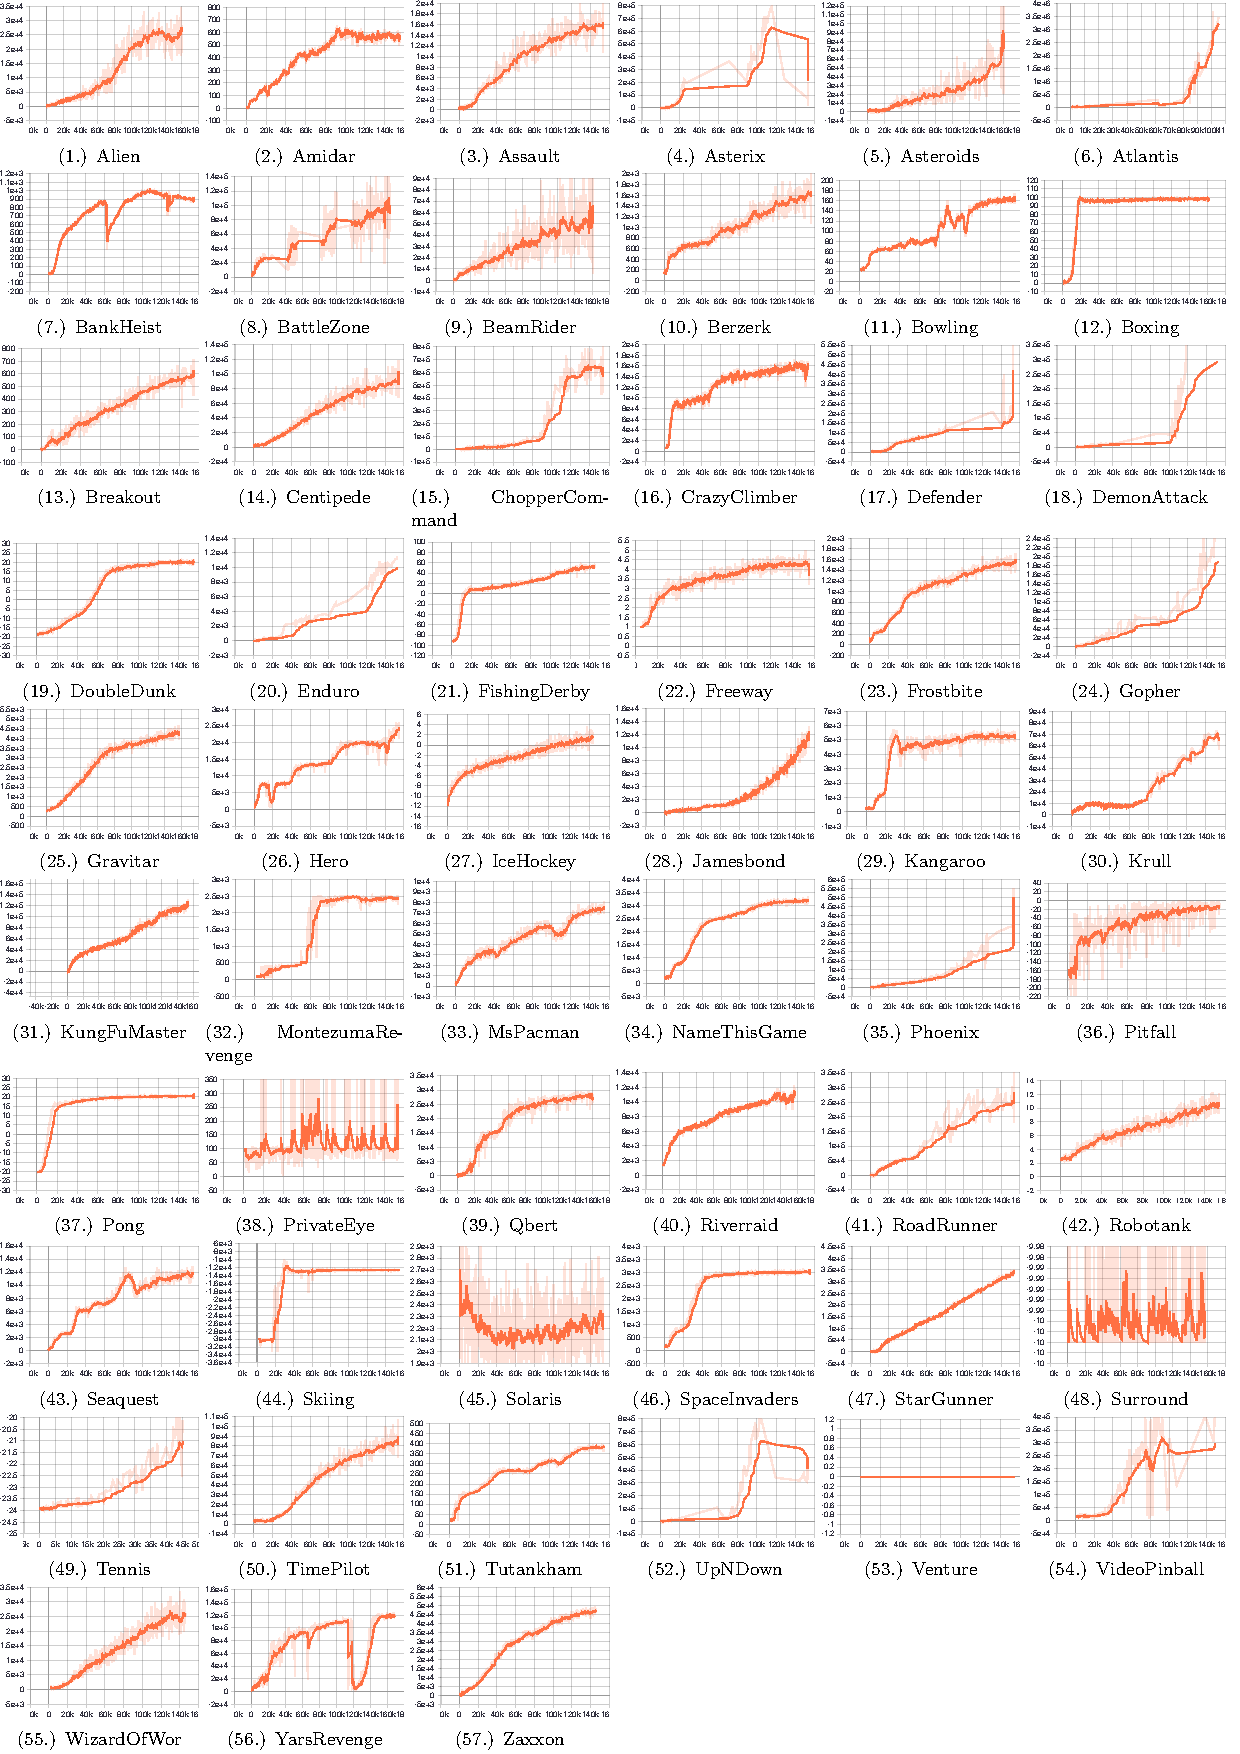
\includegraphics[width=1.0\linewidth]{body/all_fig3.pdf}
\end{figure*}

\clearpage


	\clearpage
\end{document}